\documentclass{beamer}
\usetheme{}
\usecolortheme{dolphin}           
\useinnertheme{circles}
\setbeamertemplate{itemize items}[default]
\setbeamertemplate{enumerate items}[default]
\usepackage[T1]{fontenc}
\usepackage[utf8]{inputenc}
\usepackage{lmodern}
\usepackage{amsmath}
\usepackage{booktabs} 
\usepackage{graphicx}        
\usepackage{array}
\usepackage{color}
\usepackage{textcomp}
\usepackage{epstopdf}                     % For EPS figures
\makeatletter
\def\zapcolorreset{\let\reset@color\relax\ignorespaces}
\def\colorrows#1{\noalign{\aftergroup\zapcolorreset#1}\ignorespaces}
\makeatother
\graphicspath{{/home/swl/Dropbox/ucd/international_trade/tex/}} 
\setbeamertemplate{navigation symbols}{}

%--------------------------------------
%%%% DETAILS TITLE PAGE %%%%
%--------------------------------------
\title{Trade policy}
\author{School of Economics, University College Dublin}
\date{Autumn 2017}
\begin{document}
%--------------------------------------
%%%% TITLE SLIDE %%%%
%--------------------------------------
\begin{frame}
\titlepage  
\end{frame}

%--------------------------------------
\begin{frame}
  \begin{figure}
    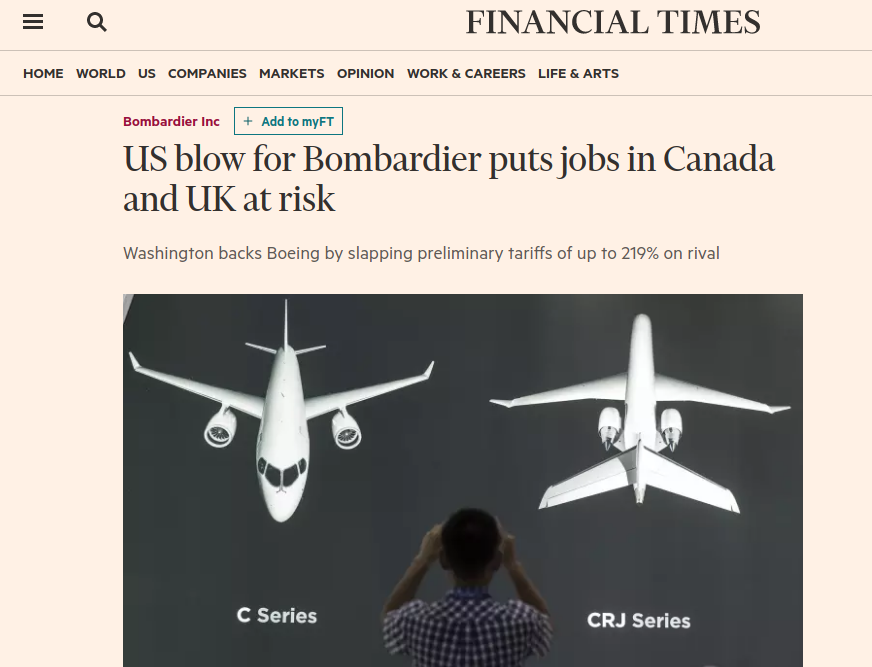
\includegraphics[scale=.3]{bombardier.png}
  \end{figure}
\end{frame}
%--------------------------------------

%--------------------------------------
\begin{frame}
  \begin{figure}
    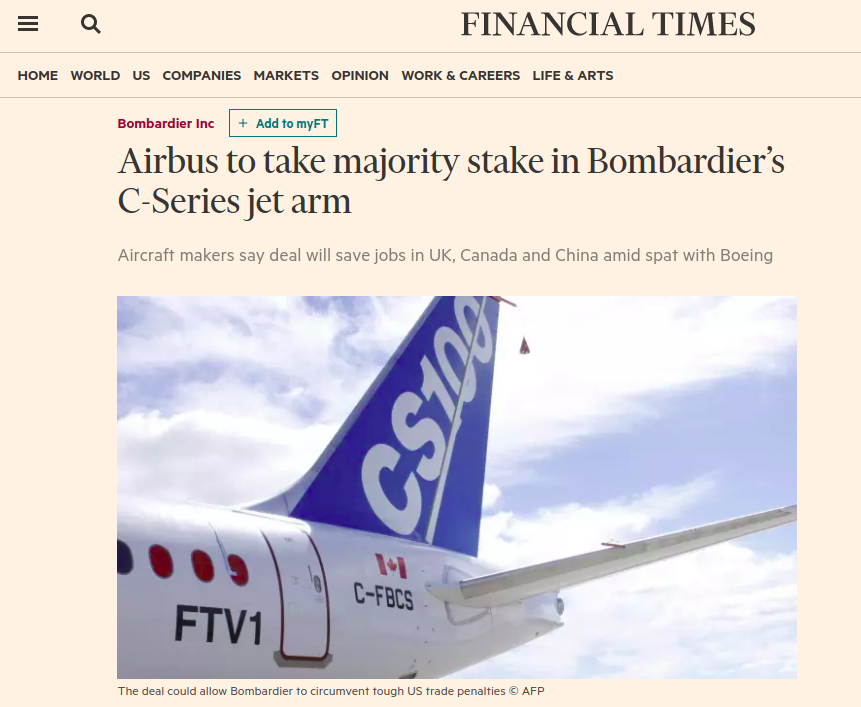
\includegraphics[scale=.3]{bombardier2.png}
  \end{figure}
\end{frame}
%--------------------------------------

%--------------------------------------
\begin{frame}
  The first lectures of this course focused on the general equilibrium
  \begin{itemize}
    \item Start with market structure, factor endowments, available technology
    \item All prices determined in equilibrium by conditions such as trade balance, marginal cost, etc.
    \item Analyse income and substitution effects
  \end{itemize}
  \medskip
  Analysis of trade policy focuses on partial equilibrium
  \begin{itemize}
    \item Only concerned with a single good or price
    \item Assume that neither incomes or other price changes happen
    \item Welfare is only affected by the consumption of a single good
  \end{itemize}
\end{frame}
%--------------------------------------

%--------------------------------------
\begin{frame}
 Trade policy is a way for countries to deal with the distributional consequences of trade along
 \begin{itemize}
   \item Factors, following from the HO-model
   \item Industries, following from the Specific Factors model
 \end{itemize}
\end{frame}
%--------------------------------------

%--------------------------------------
\begin{frame}
 There are a number of economic justifications for trade policy
 \begin{enumerate}
   \item Income distribution
   \item Raising revenue
   \item Protect infant industries
   \item Satisfying consumption goals
   \item National security
 \end{enumerate}
\end{frame}
%--------------------------------------

%--------------------------------------
\begin{frame}
There are also a number of justifications for trade policy that make little economic sense
\begin{enumerate}
  \item Pauper labour
  \item Fairness
  \item Nationalism
\end{enumerate}
\medskip
These don't make sense as they are based on misunderstanding of what policy might achieve. 
 \end{frame}
%--------------------------------------

%--------------------------------------
\begin{frame}
Pauper labour argument is based on idea that competing with foreign imports will drive domestic wages down.
\begin{itemize}
  \item Down to the low level of poor countries
\end{itemize}
\medskip
Ricardian model tells us that poor countries have low wages because they are less productive.
\begin{itemize}
  \item Trade will actually increase wages in trading countries
\end{itemize}
\medskip
One caveat in terms of wages is the factor price equalisation implied by the HO-model
\begin{itemize}
  \item Wage level will be above poor country but below rich country
\end{itemize}
\medskip
Research suggests that much of wage difference is due to technological differences, preventing PFE.
\end{frame}
%--------------------------------------

%--------------------------------------
\begin{frame}
 Some argue that it is unfair to make workers compete with workers who are either
 \begin{itemize}
   \item More productive
   \item Lower paid
 \end{itemize}
 \medskip
 Trade is not a zero-sum gain as there are benefits for both countries. 
\end{frame}
%--------------------------------------

%--------------------------------------
\begin{frame}
  The nationalist argument entails that one should buy from home producers so that the benefits won't go to foreigners.
  \begin{itemize}
    \item Confuses costs and benefits as households benefit from consumption and producers incur production costs
  \end{itemize}
  \medskip
  One would be better of import cheaper goods paid for with exports. 
\end{frame}
%--------------------------------------

%--------------------------------------
\begin{frame}  
  In most cases protectionist measures are a second best
  \begin{itemize}
    \item Way to cope with market imperfections
    \item Provide time/resources for firms to undertake cost-reducing investments
    \item Compensate globalisation losers; labour allocation away from declining industries
  \end{itemize}
\end{frame}
%--------------------------------------

%--------------------------------------
\begin{frame}
  Set policy is often the result of various drivers
  \begin{itemize}
    \item Special interest groups
    \item Distortion created by voting; e.g. over-representation of rural areas    
  \end{itemize}
  \medskip
  The political economy aspects of trade we will discuss in more detail next lecture.  
\end{frame}
%--------------------------------------

%--------------------------------------
\begin{frame}
Most common type of trade protection are tariffs which often play an important fiscal role as it provides a source of income
  \begin{itemize}
    \item American budget depended on tariffs until income tax was introduced in 1913
    \item Many developing countries lack fiscal capabilities and need tariffs to augment their budget
  \end{itemize}
\end{frame}
%--------------------------------------

%--------------------------------------
\begin{frame}{Average tariff rate and revenue}
\framesubtitle{source: WDI}
  \begin{figure}
    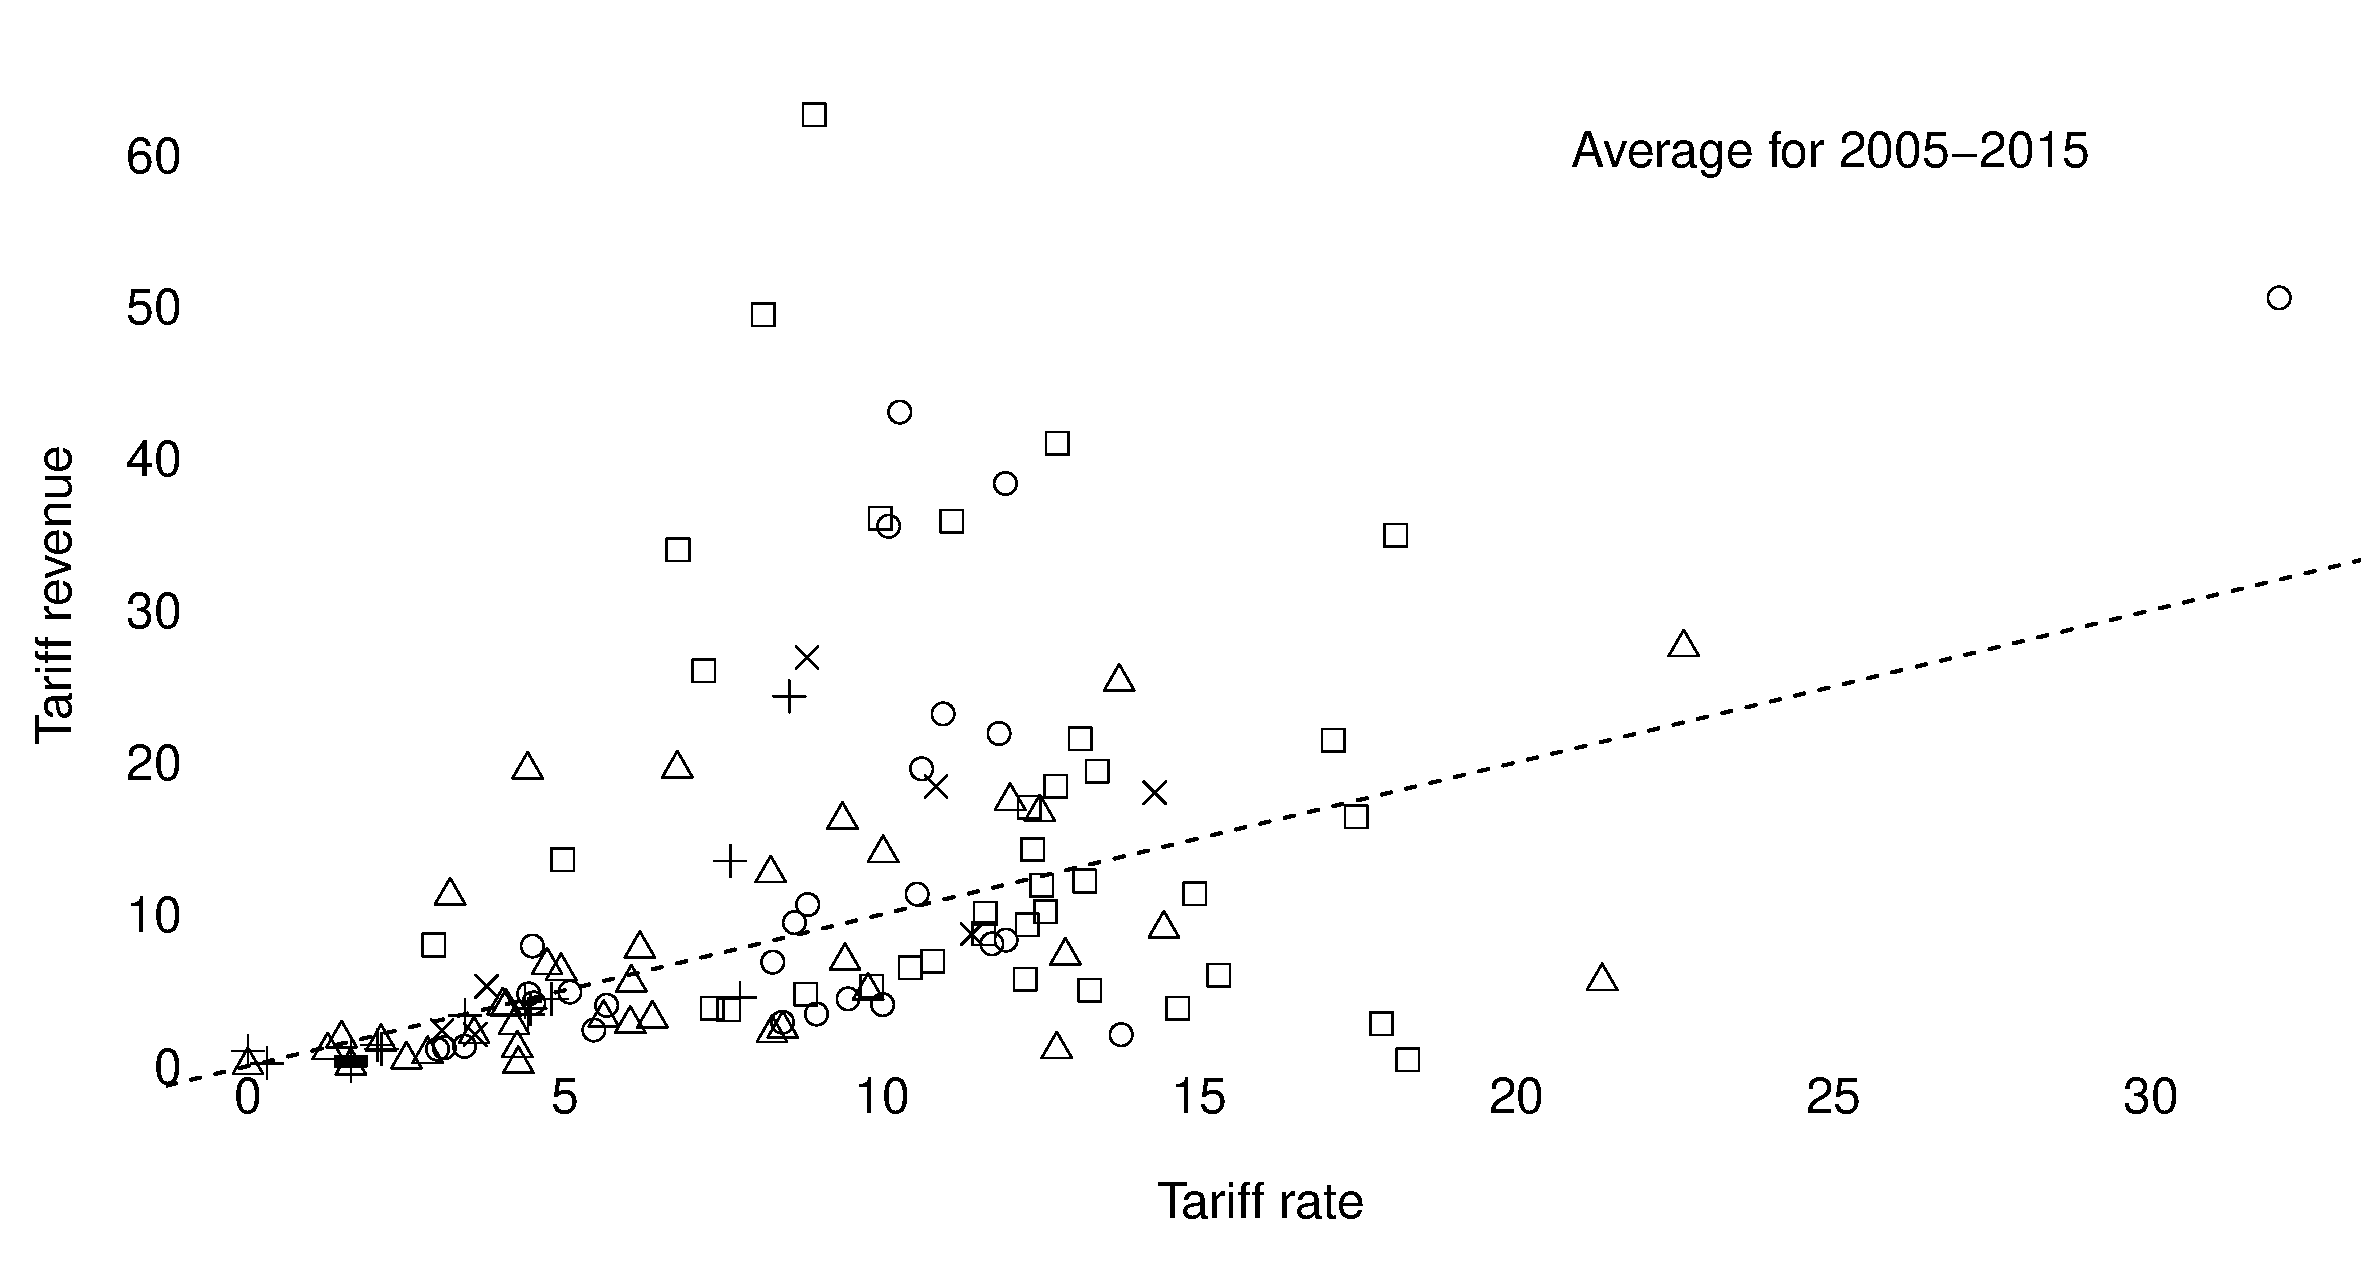
\includegraphics[scale=.25]{tariff}
  \end{figure}
\end{frame}
%--------------------------------------

%--------------------------------------
\begin{frame}
  Tariffs are taxes levied on imported goods, there are two types
  \begin{enumerate}
    \item Ad valorem tariff; based on the value of the imported good (e.g. 10\% of wheat imports)
    
    \begin{align*}
      p=p_w(1+\tau)
    \end{align*}

    \item Specific tariff; fixed charge for each unit of imported good (eg. 5 euro per barrel of oil)
    
    \begin{align*}
      p=p_w+\tau
    \end{align*}    
  \end{enumerate}
\end{frame}
%--------------------------------------

%--------------------------------------
\begin{frame}
 \begin{itemize}
   \item[Q:] How are tariffs implemented?
   \item[A:] At the border. 
 \end{itemize}
 \medskip
 By custom officers who will determine
 \begin{itemize}
   \item The type of good
   \item The price to use for ad valorem tariffs
 \end{itemize}
 \medskip
 NB - custom officers can, sometimes, be bribed.  
\end{frame}
%--------------------------------------

%--------------------------------------
\begin{frame}
  \begin{figure}
    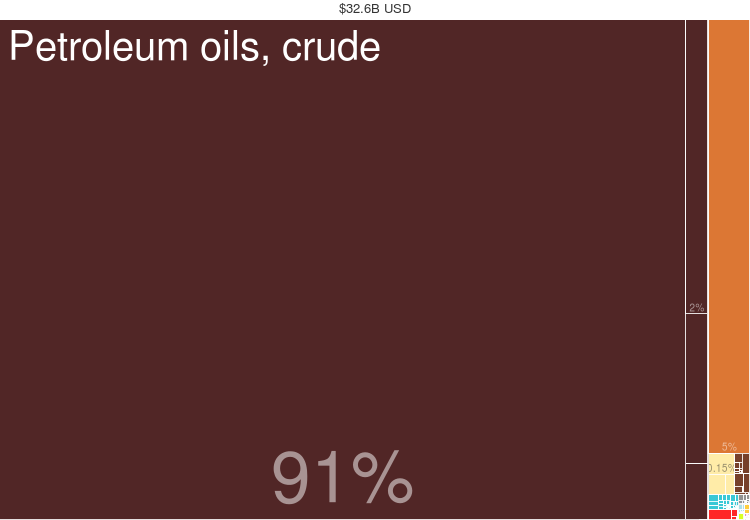
\includegraphics[scale=.4]{angola2.png}
  \end{figure}
\end{frame}
%--------------------------------------

%--------------------------------------
\begin{frame}
  Angola is the second largest oil exporter in Africa meaning a large influx of foreign reserves.
  This makes Luanda, the capital, one of the most expensive cities in the world.
  In 2014 the government imposed tariffs in order to diversify the economy.
  \begin{itemize}
    \item Local food prices experienced a large increase
    \item Import tariffs offset the decrease in inflation
  \end{itemize}
\end{frame}
%--------------------------------------

%--------------------------------------
\begin{frame}{Comparison of food prices in Angola and the UK}
  \begin{figure}
    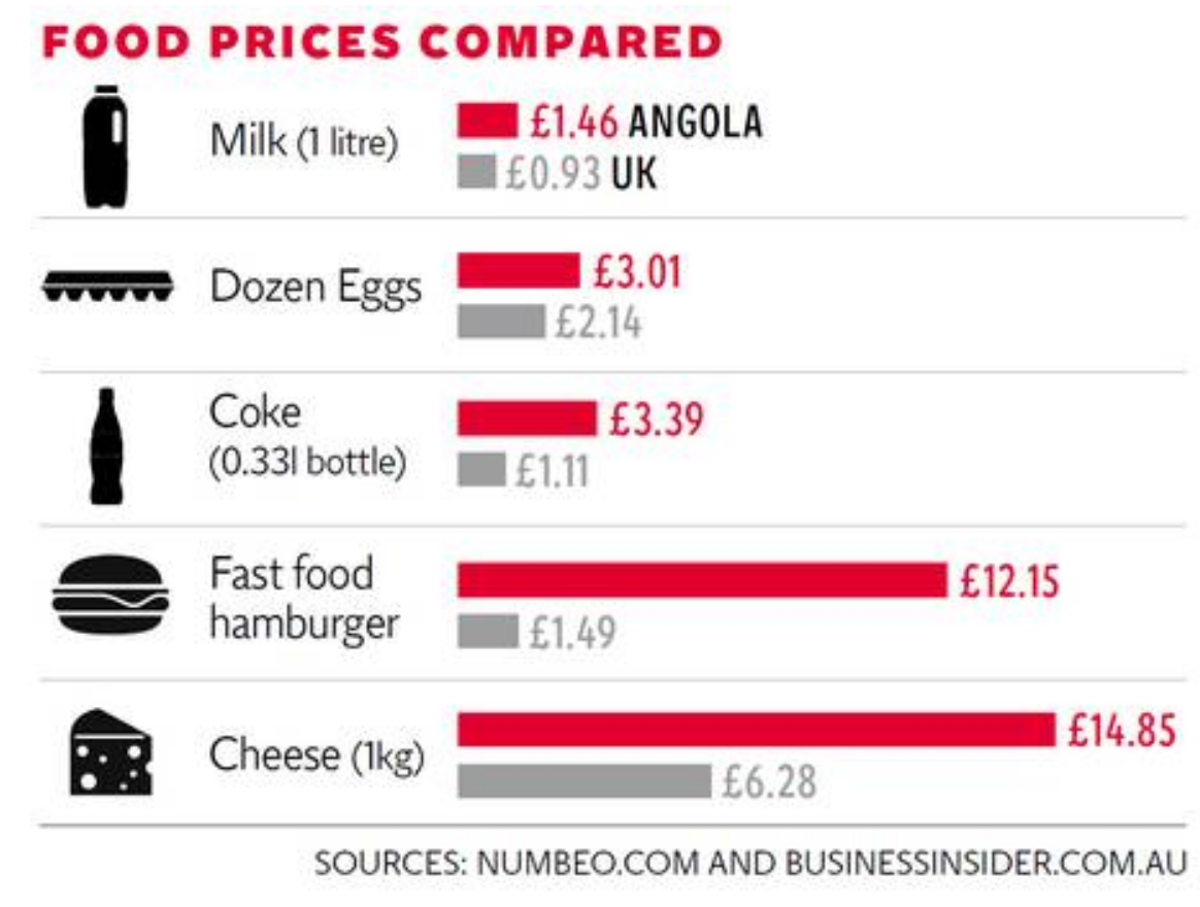
\includegraphics{angola}
  \end{figure}
\end{frame}
%--------------------------------------

%--------------------------------------
\begin{frame}
  Let's consider the effect of a tariff on the market for apples.\\ 
  In the absence of trade we have
  \begin{align*}
    p > p^*
  \end{align*}
  \medskip
  Allowing trade apples will be exported from $Foreign$ to $Home$ until
  \begin{align*}
    p = p^*
  \end{align*}
  \medskip
  $Home$ import demand and $Foreign$ export supply are given by
  \begin{align*}
    MD=D-S\\
    XS^*=S^*-D^*
  \end{align*}
\end{frame}
%--------------------------------------

%--------------------------------------
\begin{frame}{$Home$ import demand curve}
  \begin{figure}
    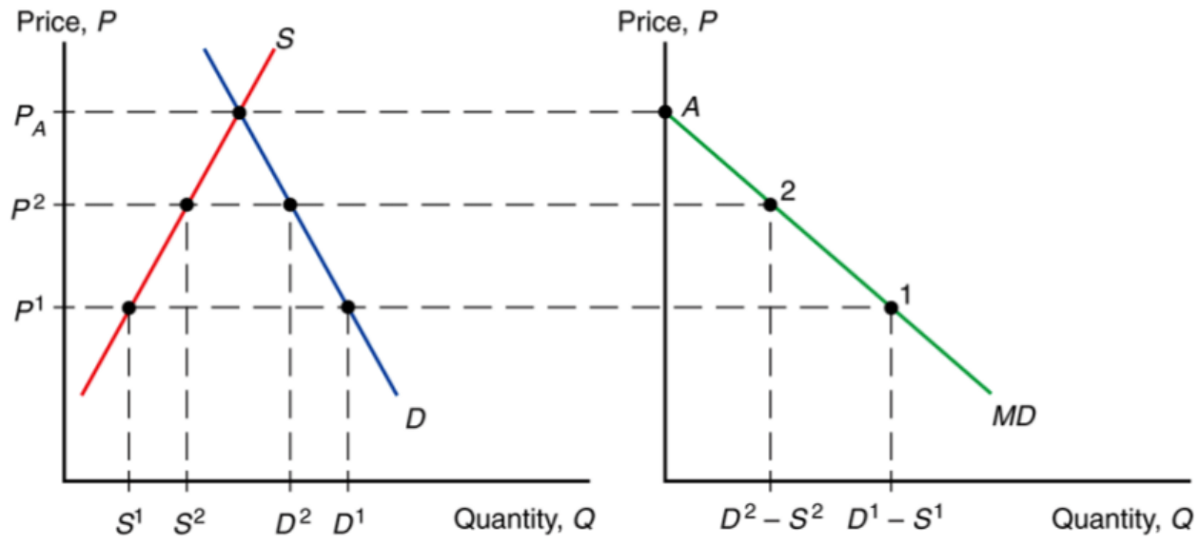
\includegraphics{home_demand}
  \end{figure}  
\end{frame}
%--------------------------------------

%--------------------------------------
\begin{frame}{$Foreign$ export supply}
  \begin{figure}
    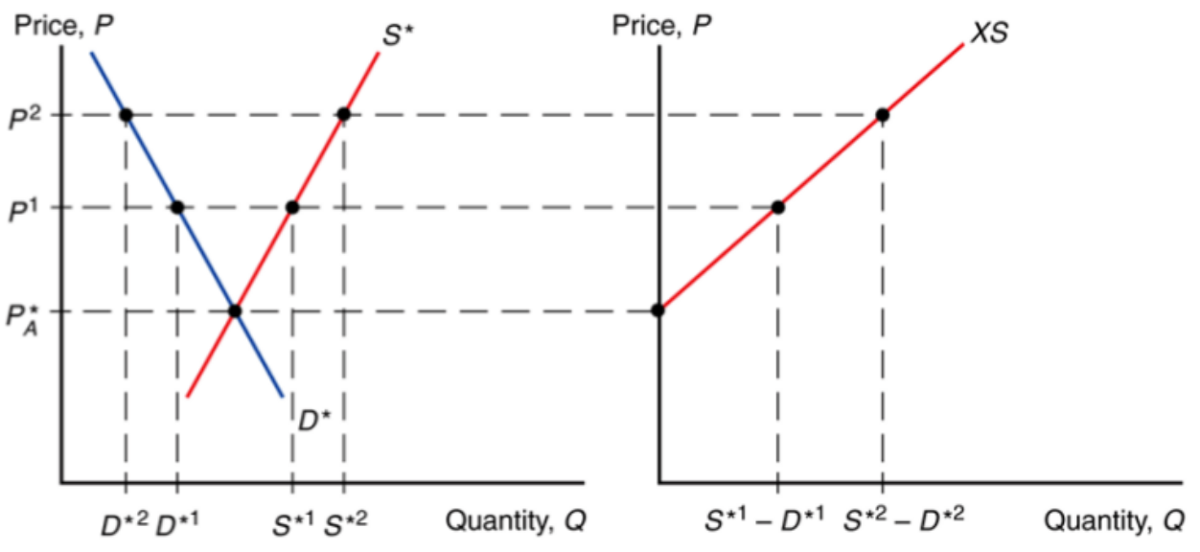
\includegraphics{export_supply}
  \end{figure}  
\end{frame}
%--------------------------------------

%--------------------------------------
\begin{frame}
  When the world market is in equilibrium we have that import demand equals export supply or
  \begin{align*}
    D-S=S^*-D^*
  \end{align*}
  Which entails that world demand equals world supply
  \begin{align*}
    D+D^*=S+S^*
  \end{align*}
\end{frame}
%--------------------------------------

%--------------------------------------
\begin{frame}{World equilibrium}
  \begin{figure}
    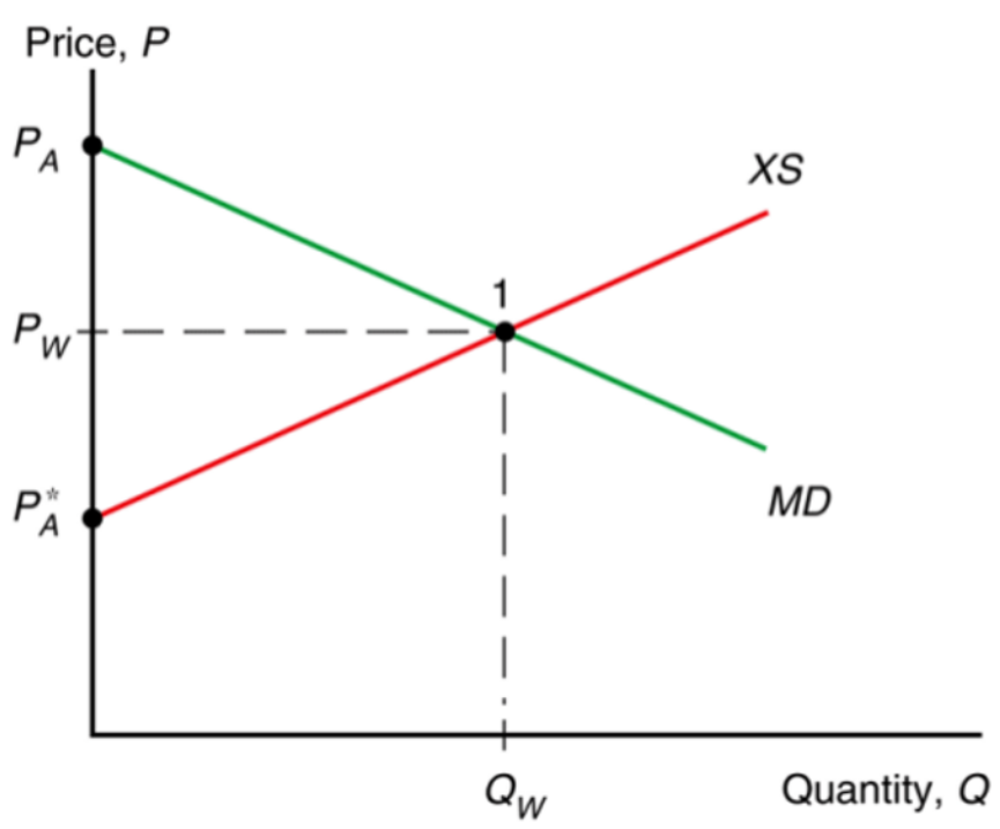
\includegraphics{world_eq}
  \end{figure}
\end{frame}
%--------------------------------------

%--------------------------------------
\begin{frame}
Let's assume that for some reason $Home$ government decides to implement tariff $\tau$. 
$Home$ producers will export only when  
  \begin{align*}
    p +\tau \leq p^*
  \end{align*}
  \medskip
  Whereas they only sell domestically if
  \begin{align*}
    p +\tau \geq p^*
  \end{align*}
  \medskip
  The equilibrium price difference will be the tariff
  \begin{align*}
    p_t-p_t^*=\tau
  \end{align*}
  \medskip
  Meaning that the tariff acts as a transportation cost.   
\end{frame}
%--------------------------------------


%--------------------------------------
\begin{frame}
  After the tariff is set there will be excess demand in $Home$ and excess supply in $Foreign$, as a result
  \begin{enumerate}
    \item $p$ will increase and $p^*$ will decrease
    \item Both $Home$ imports and $Foreign$ exports will decrease
  \end{enumerate}  
\end{frame}
%--------------------------------------

%--------------------------------------
\begin{frame}{Effect of tariff}
  \begin{figure}
    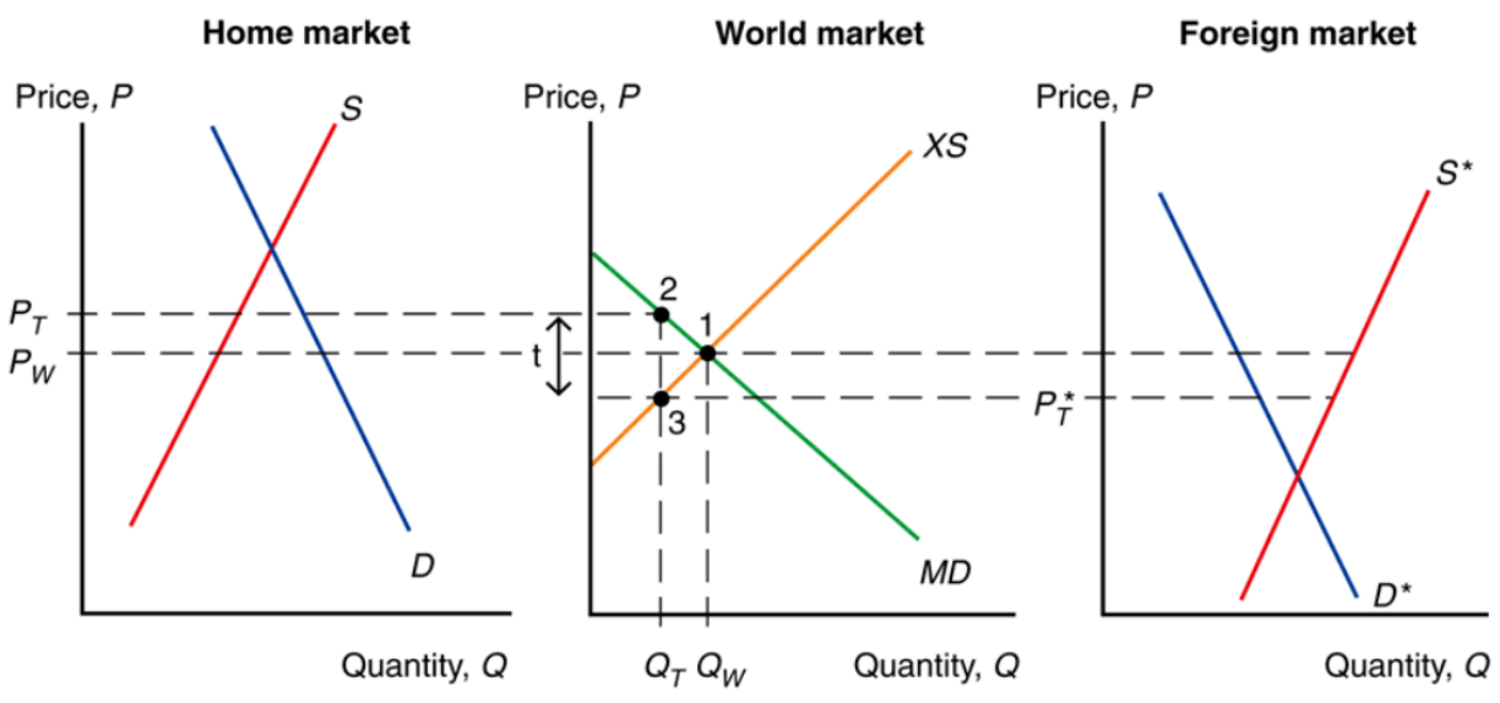
\includegraphics[scale=.8]{tariff_effect}
  \end{figure}
\end{frame}
%--------------------------------------

%--------------------------------------
\begin{frame}
  Due to the tariff the price in $Home$ will increase from $p_{w}$ to $p_t$ and as a result producers will supply more while consumers demand less.
  \begin{itemize}    
    \item Import quantity drop from $Q_w$ to $Q_t$ (2)
  \end{itemize}
  \medskip
  In $Foreign$ the price will drop from $p_w$ to $p_t^*$ which means that producers will supply less and consumers demand more.
  \begin{itemize}    
    \item Export quantity decreases from $Q_w$ to $Q_t$ (3)
  \end{itemize}
  \medskip
  When $p_t-p_t^*=\tau$ we have $MD=XS^*$
  \begin{itemize}
    \item The increase in $p_t$ can be less than the tariff
    \item Part of the tariff effect will cause $Foreign$ export price to decline, although effect is very small
  \end{itemize}
\end{frame}
%--------------------------------------

%--------------------------------------
\begin{frame}
  Of course the economic size of a country imposing a tariff matters. 
  If $Home$ is a small country it will have no effect on $p^*$ or $p_{w}$. 
  \begin{itemize}
    \item $Home$ demand is an insignificant part of world demand
  \end{itemize}
  \medskip
  When $p^*=p_{w}$ the price in $Home$ will increase by the full amount of the tariff
  \begin{align*}
    p_t=p_w+\tau
  \end{align*}
  \medskip
  The price will creep towards the price under autarky. 
\end{frame}
%--------------------------------------

%--------------------------------------
\begin{frame}{Tariff effect in small country}
  \begin{figure}
    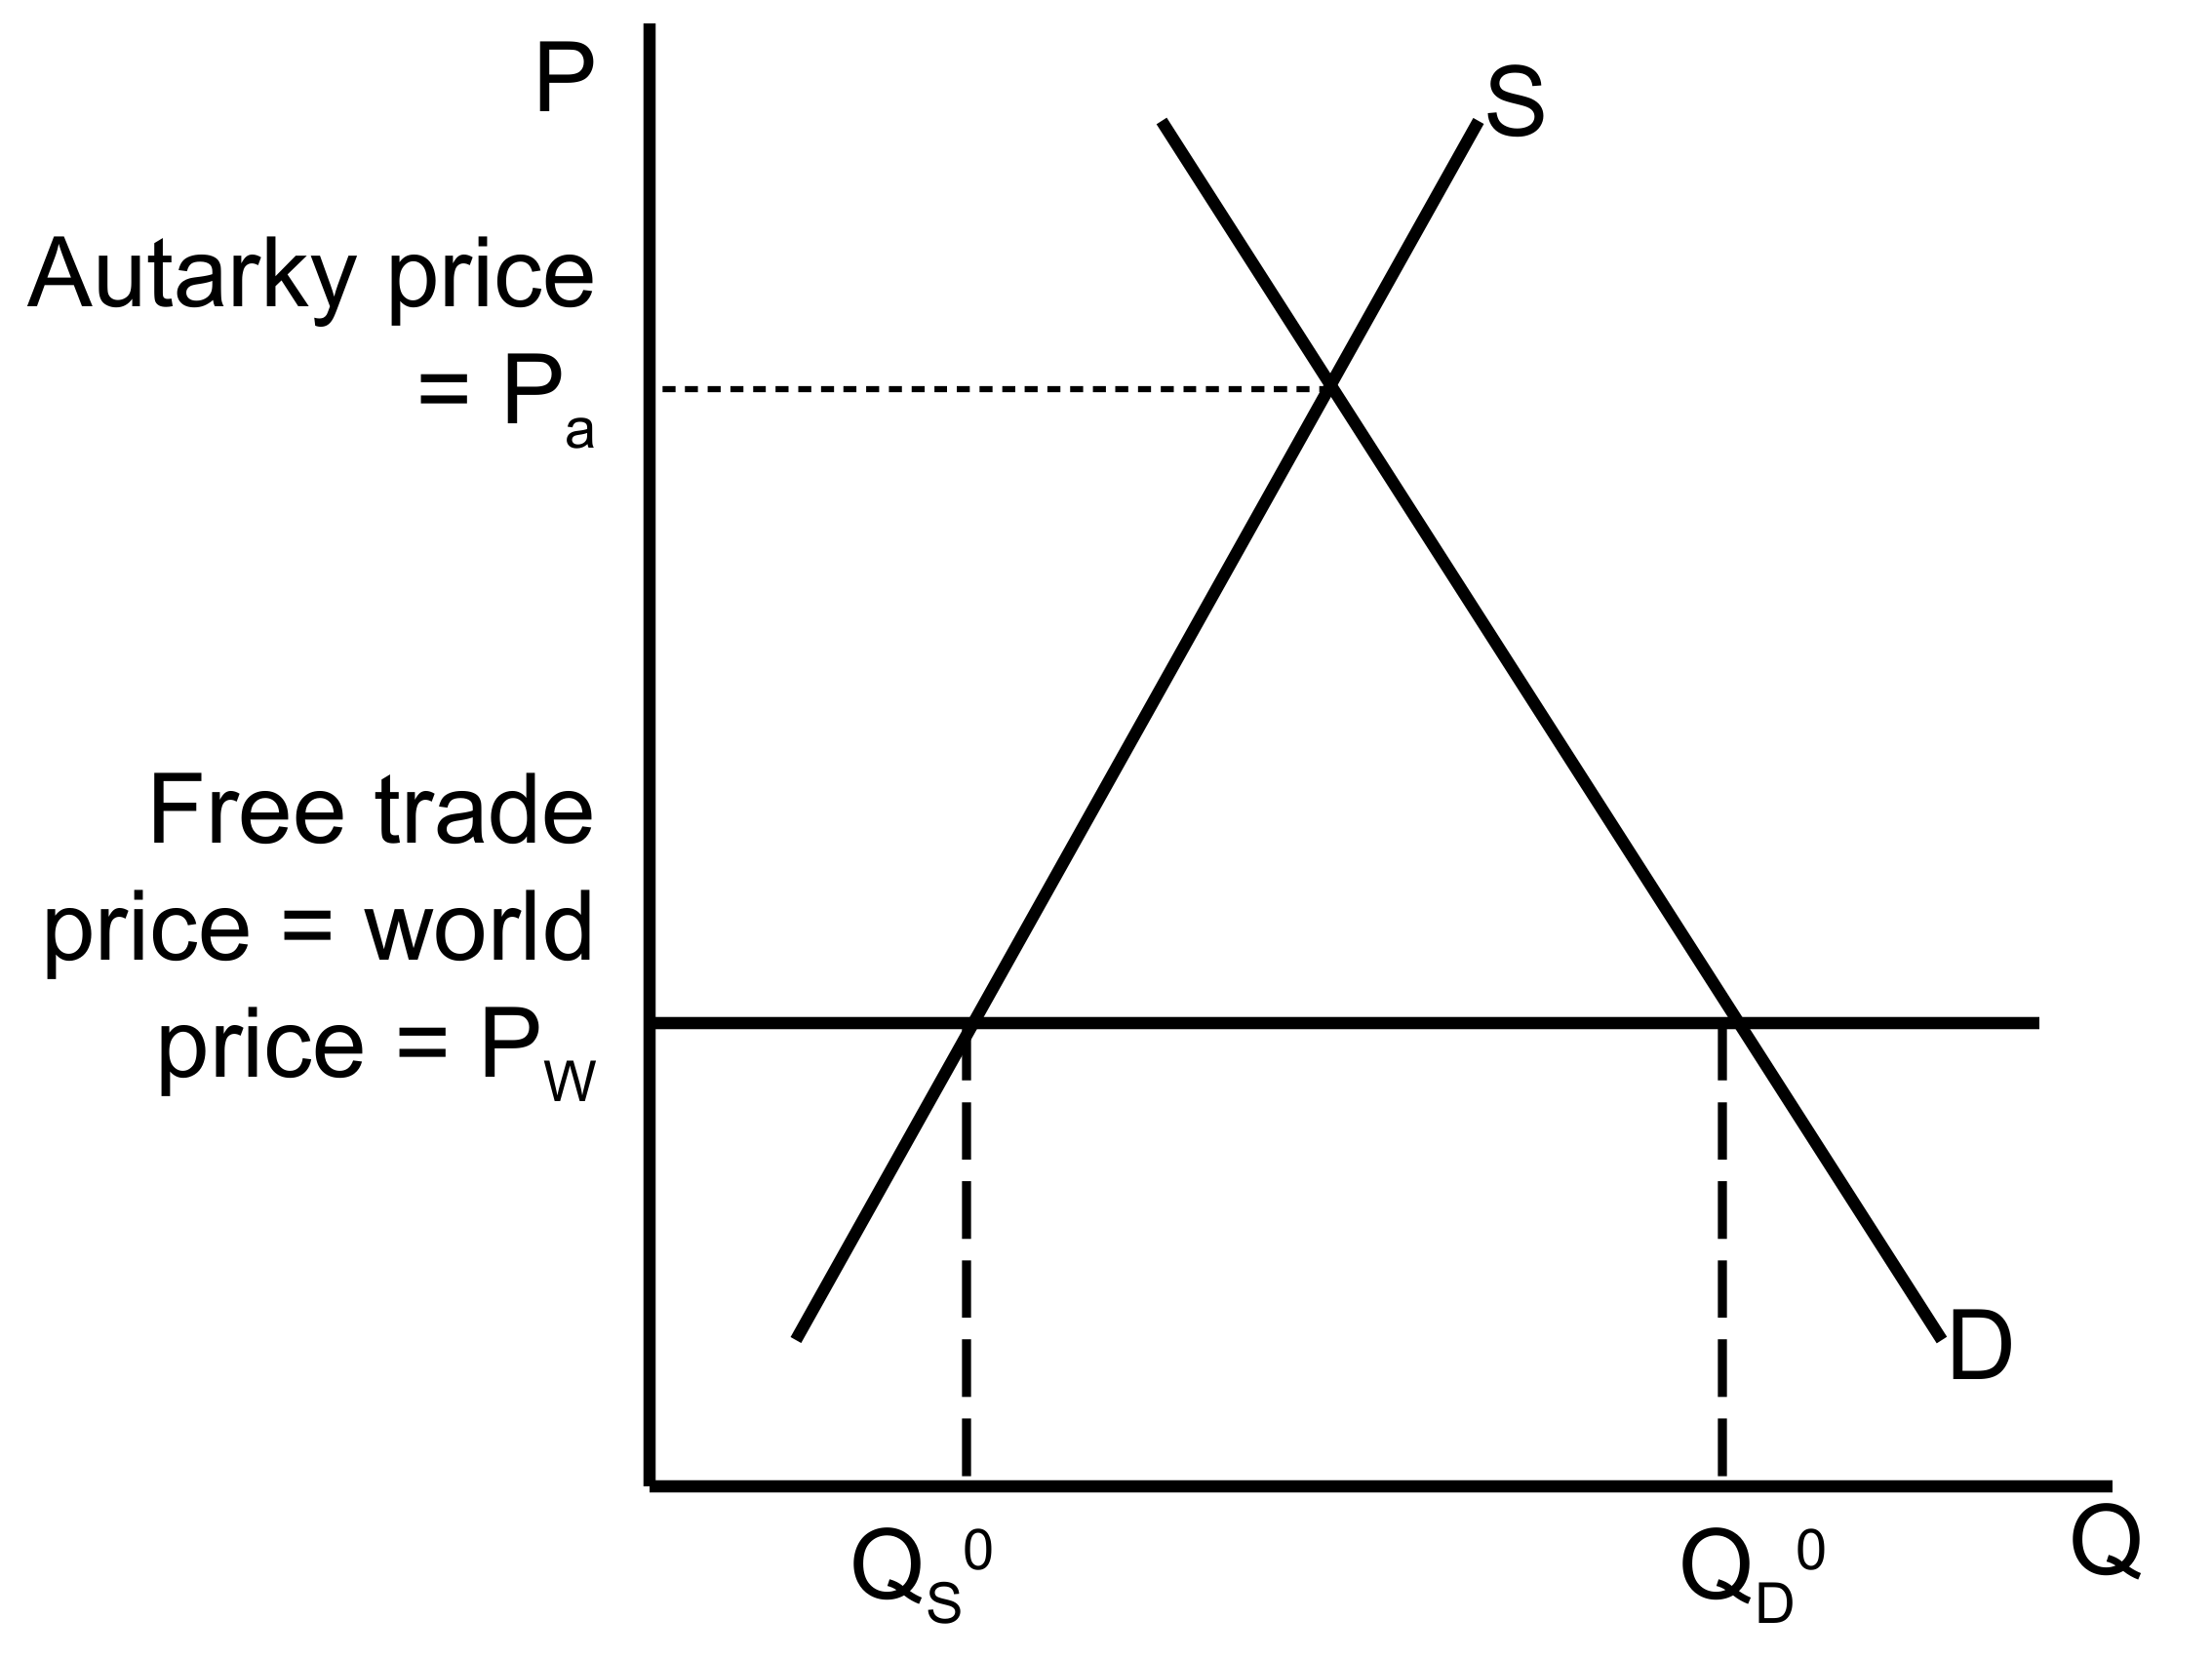
\includegraphics[scale=.5]{tariff_small_country1.png}
  \end{figure}
\end{frame}
%--------------------------------------

%--------------------------------------
\begin{frame}{Tariff effect in small country}
  \begin{figure}
    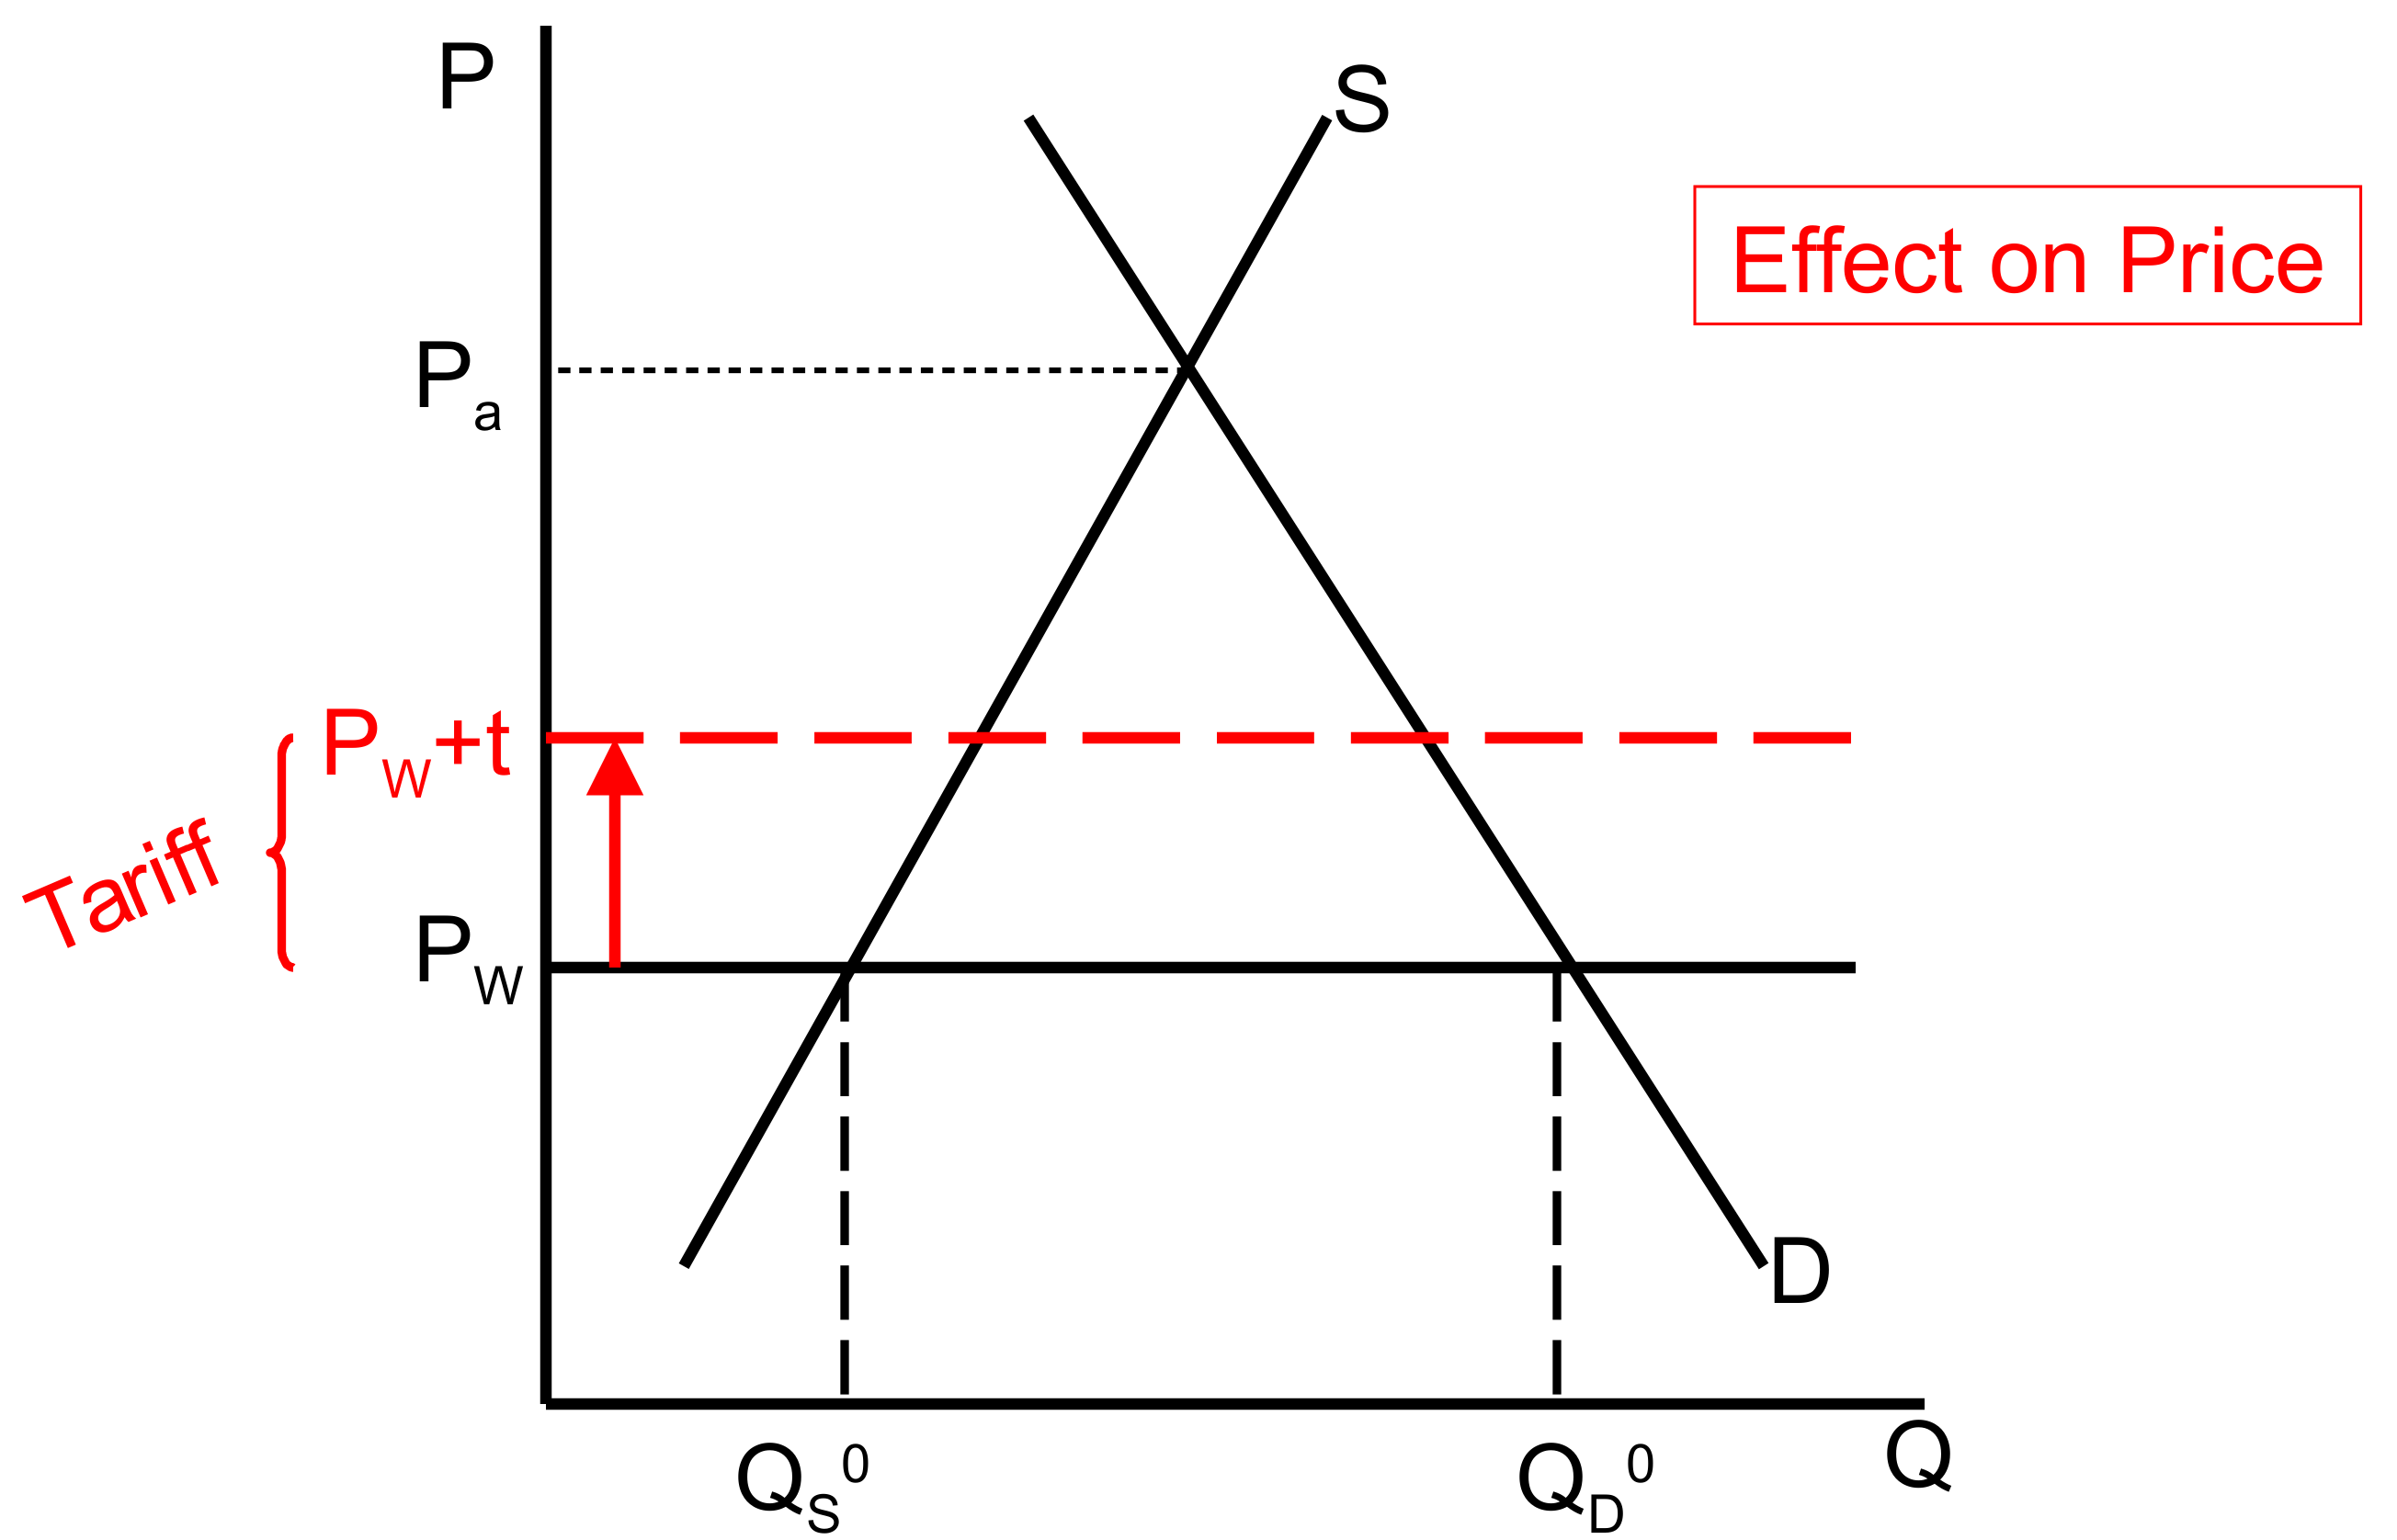
\includegraphics[scale=.5]{tariff_small_country2.png}
  \end{figure}
\end{frame}
%--------------------------------------

%--------------------------------------
\begin{frame}{Tariff effect in small country}
  \begin{figure}
    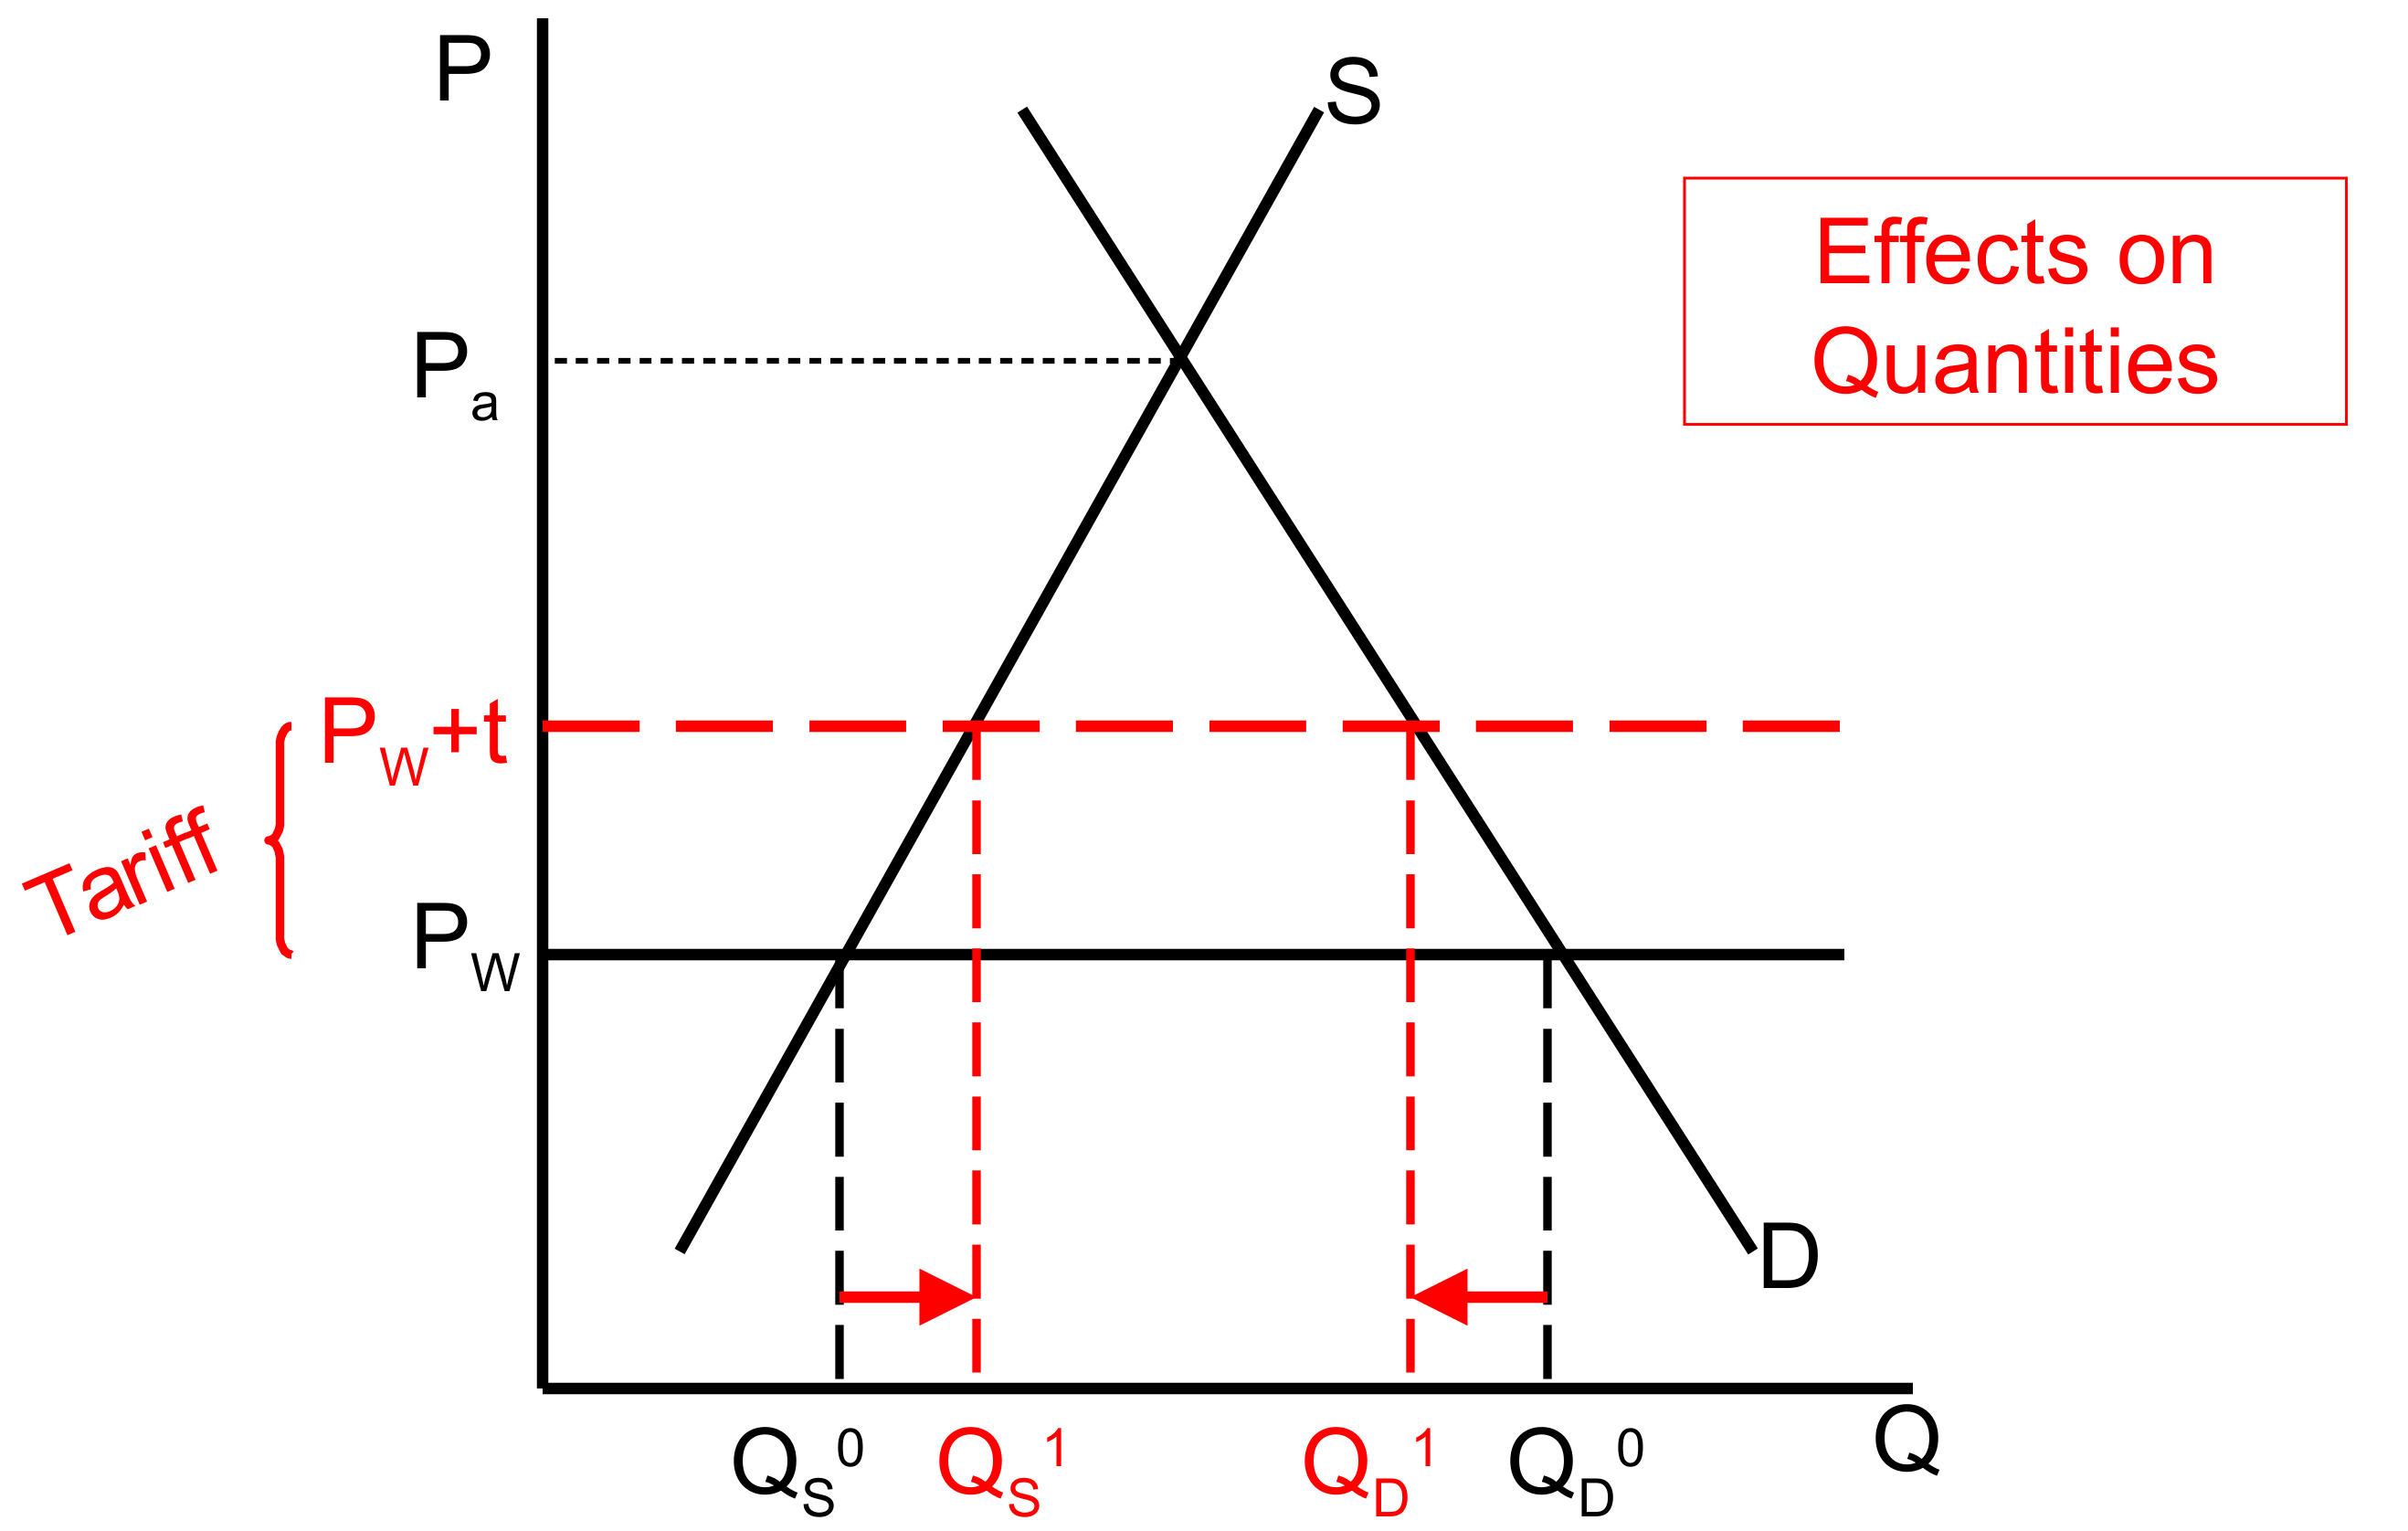
\includegraphics[scale=.5]{tariff_small_country3.png}
  \end{figure}
\end{frame}
%--------------------------------------

%--------------------------------------
\begin{frame}{Tariff effect in small country}
  \begin{figure}
    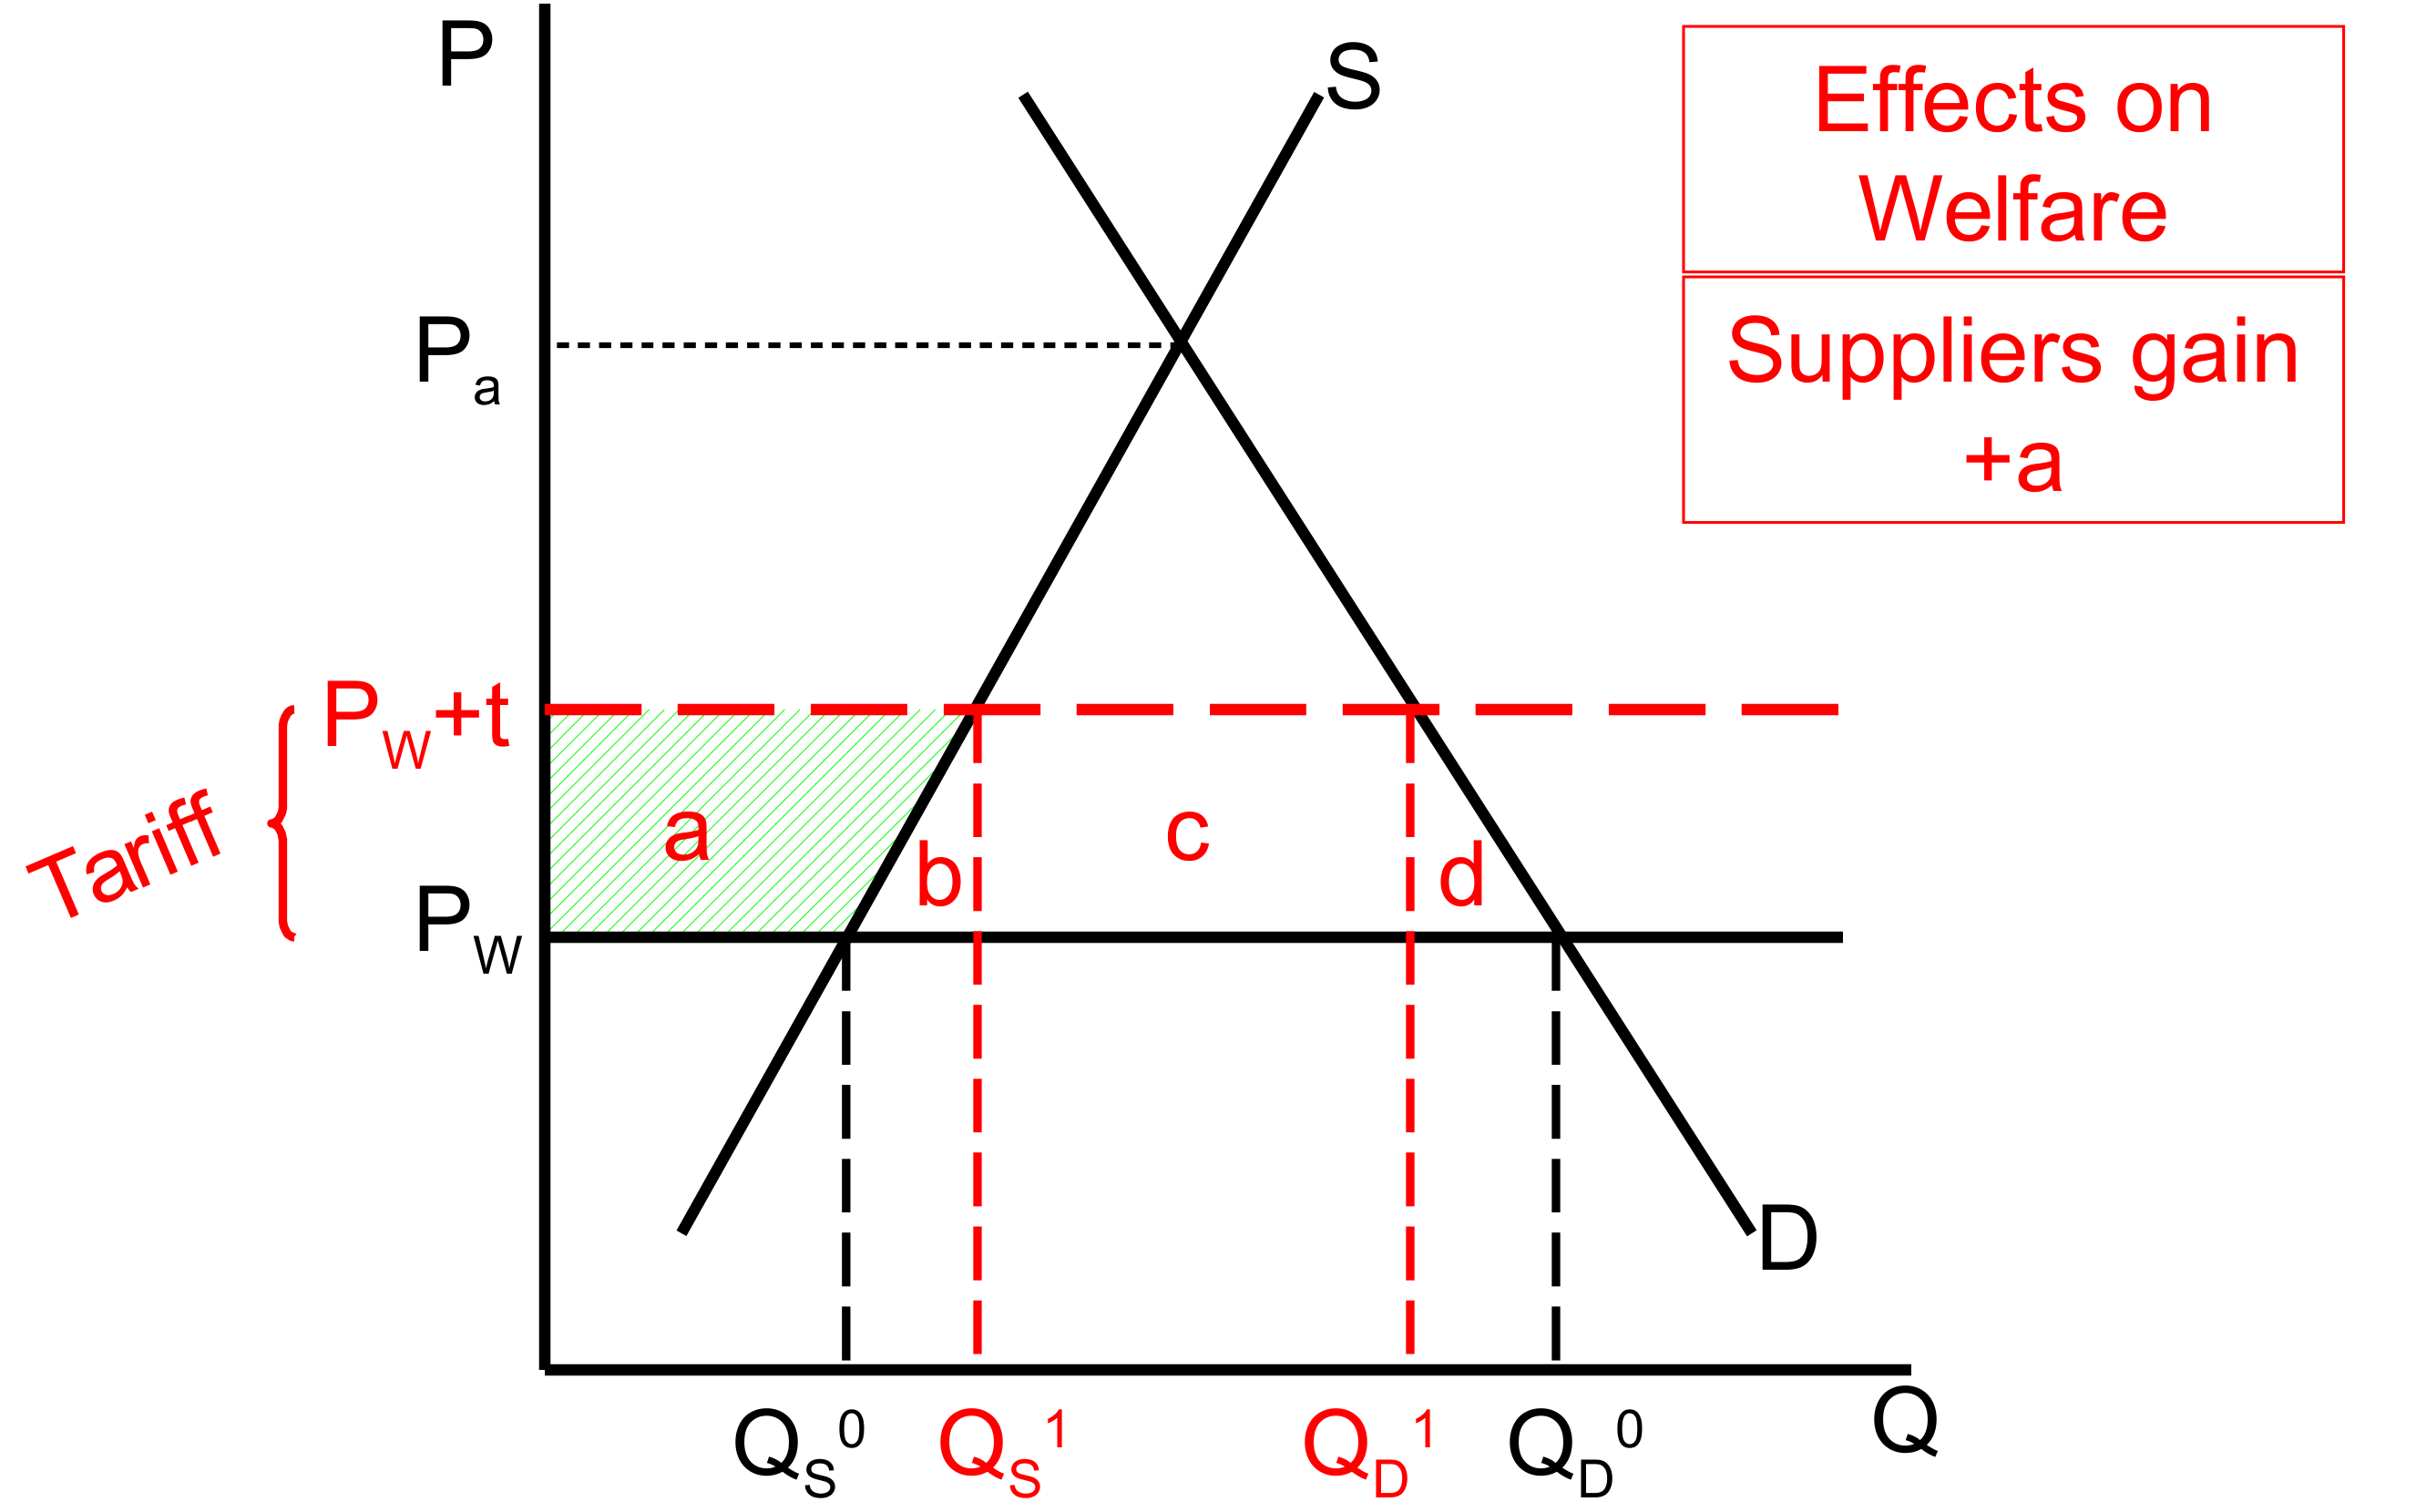
\includegraphics[scale=.5]{tariff_small_country4.png}
  \end{figure}
\end{frame}
%--------------------------------------

%--------------------------------------
\begin{frame}{Tariff effect in small country}
  \begin{figure}
    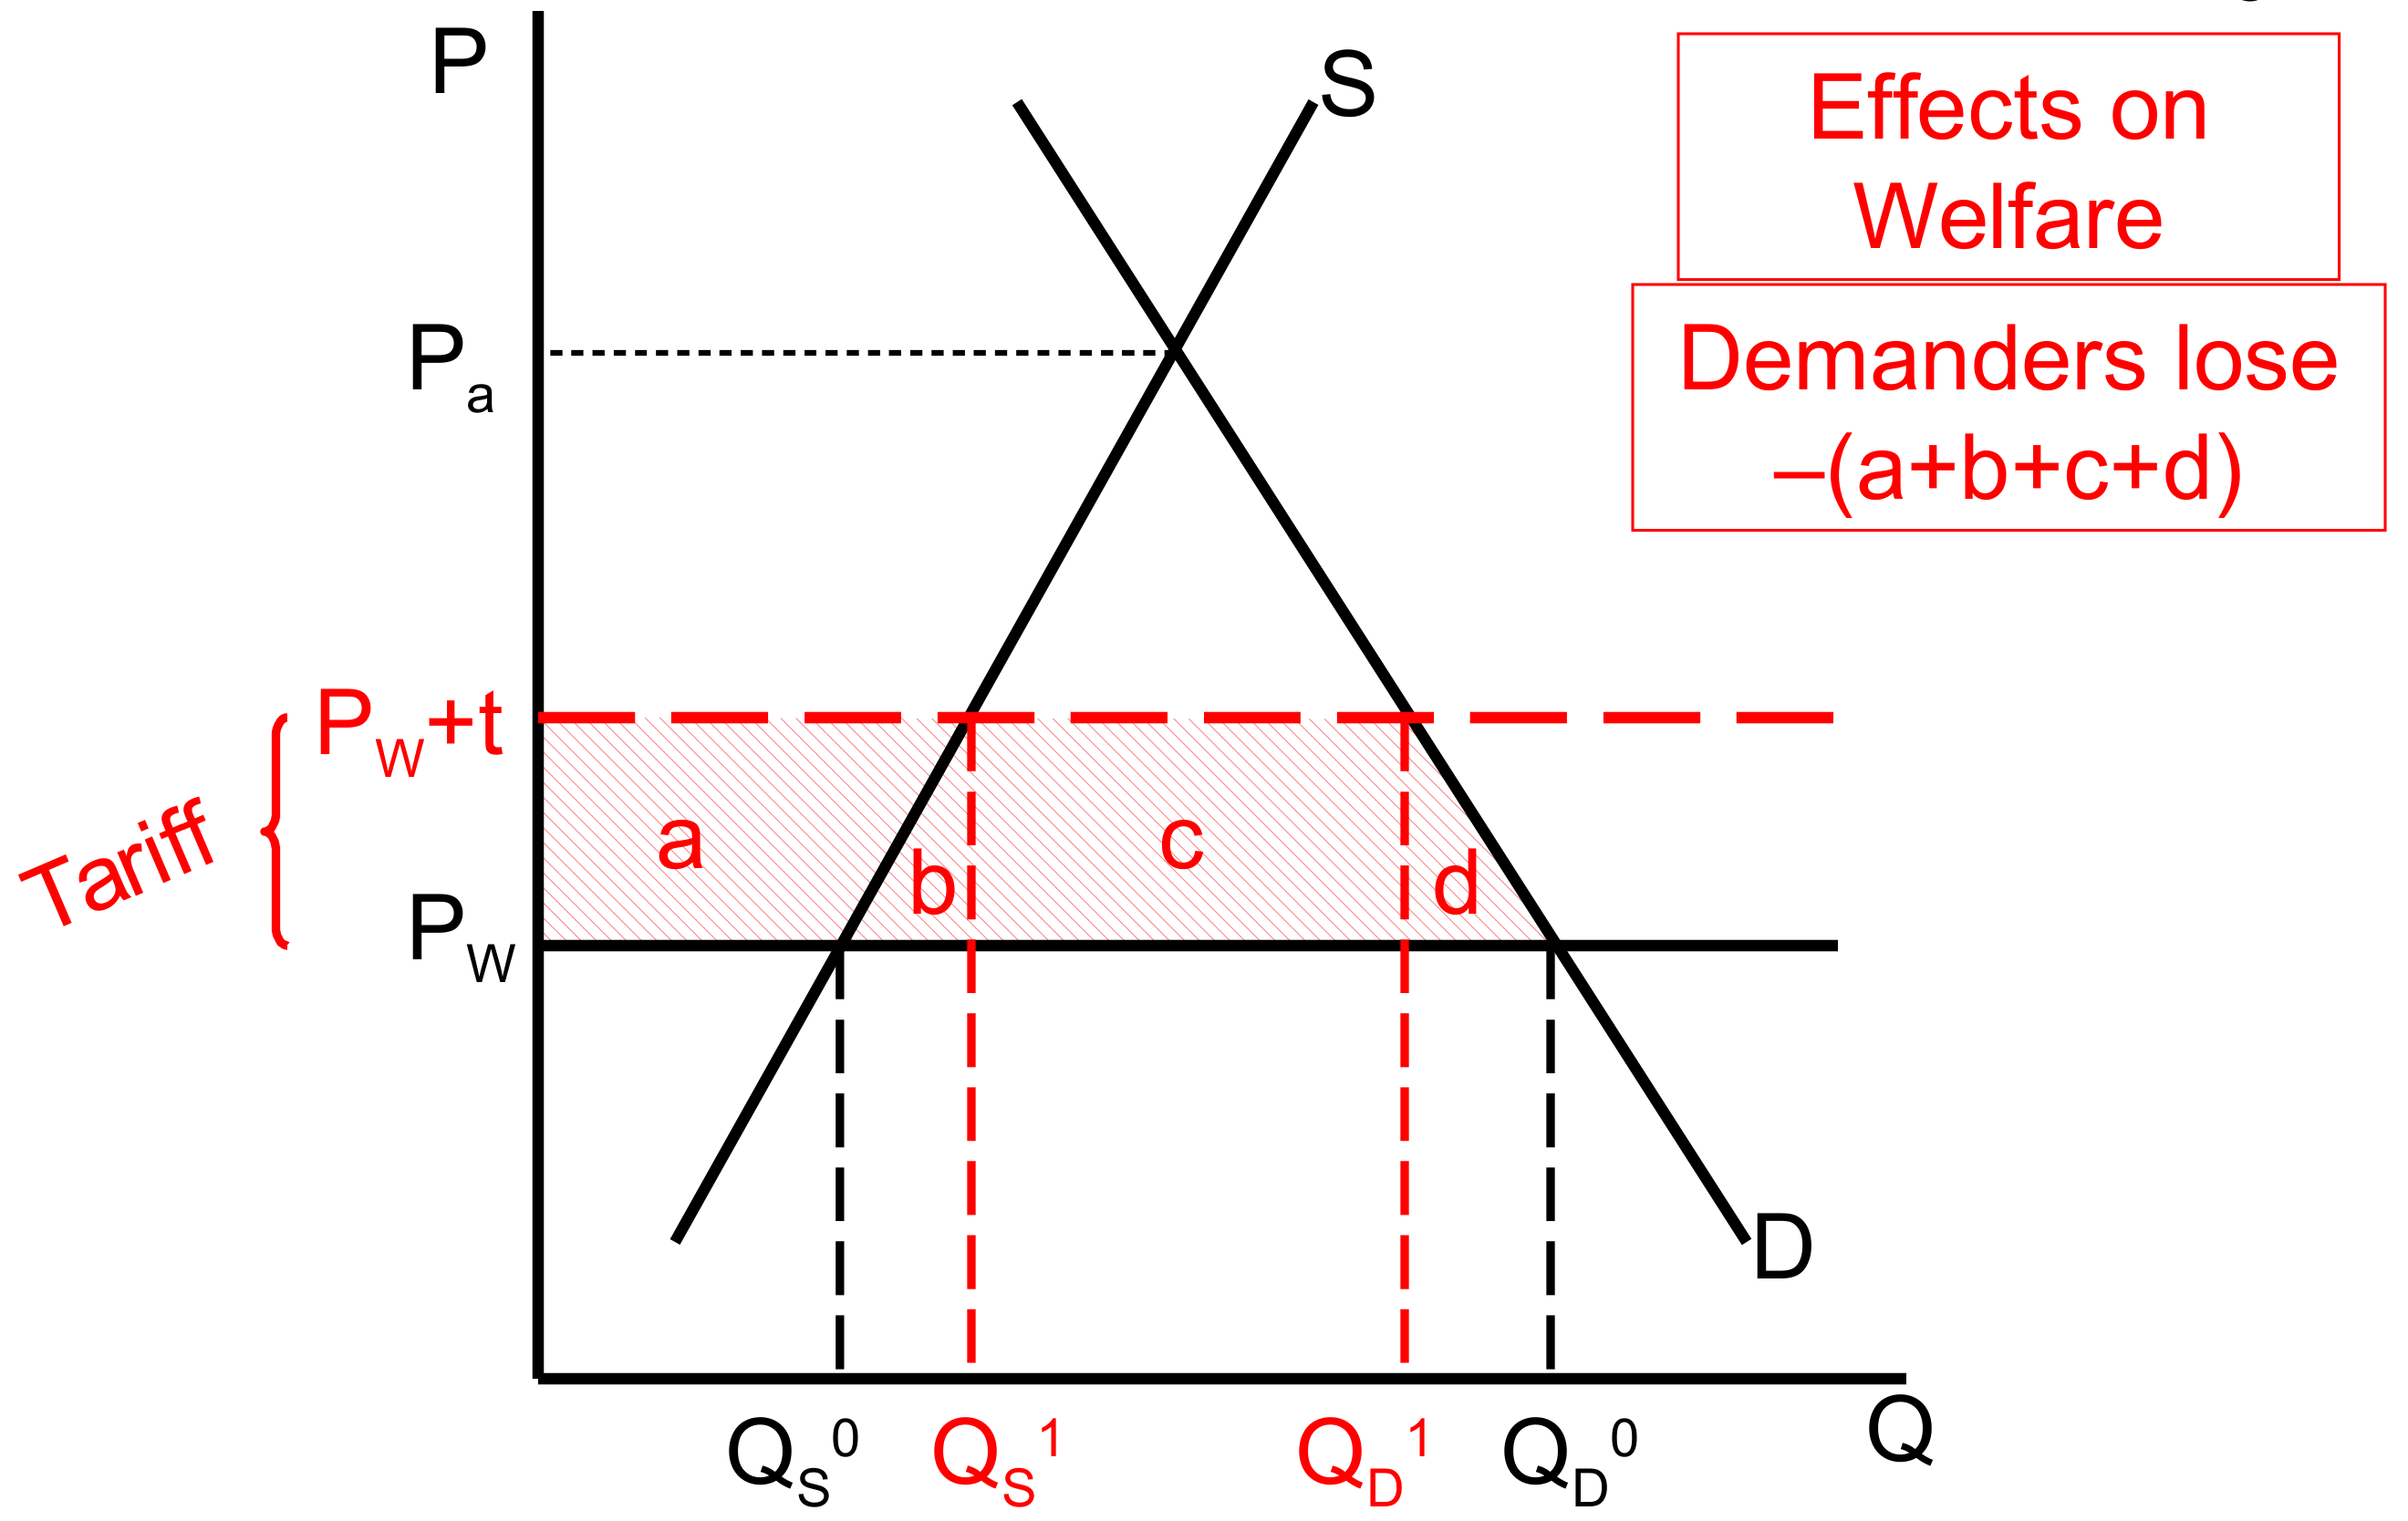
\includegraphics[scale=.5]{tariff_small_country5.png}
  \end{figure}
\end{frame}
%--------------------------------------

%--------------------------------------
\begin{frame}{Tariff effect in small country}
  \begin{figure}
    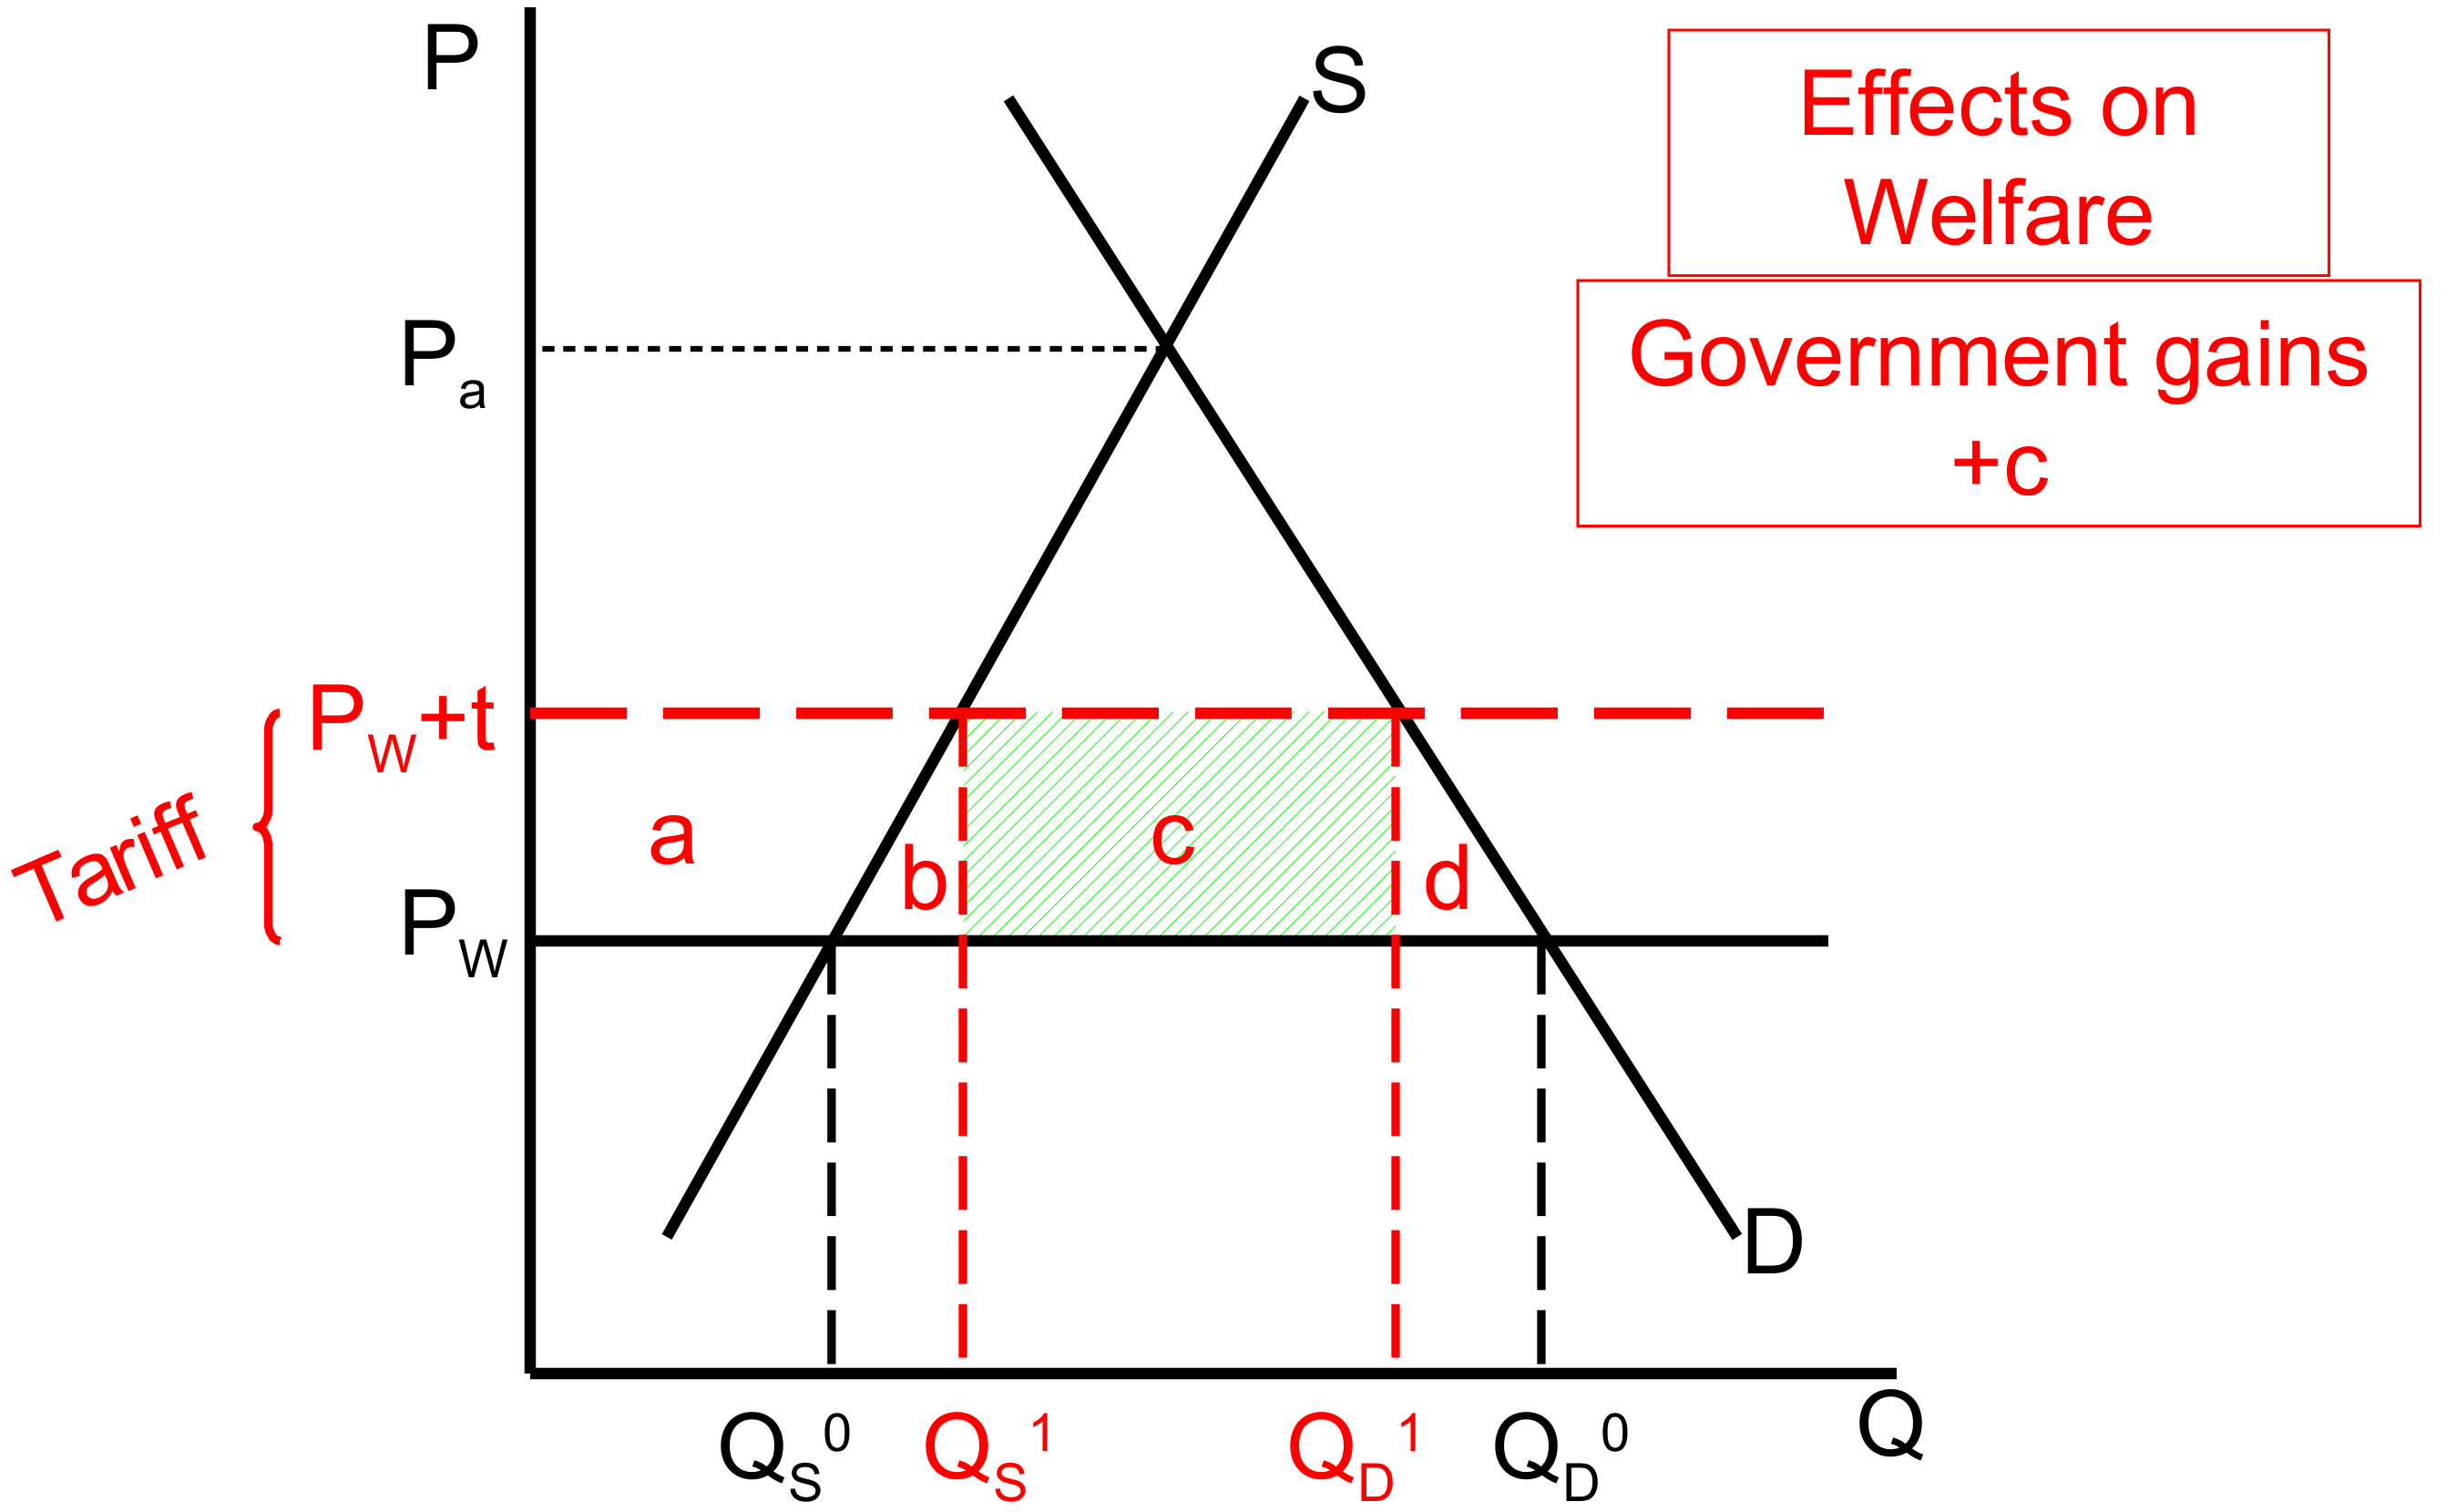
\includegraphics[scale=.5]{tariff_small_country6.png}
  \end{figure}
\end{frame}
%--------------------------------------

%--------------------------------------
\begin{frame}
  In a small country the effect of a tariff is that there will be fewer imports and more domestic production. 
  Welfare loss will be determined by the
  \begin{itemize}
    \item Production distortion loss
    \item Consumption distortion loss
  \end{itemize}
  \medskip
  Goverment will experience an increase in income due to tariff revenues.
\end{frame}
%--------------------------------------

%--------------------------------------
\begin{frame}{Tariff effect in small country}
  \begin{figure}
    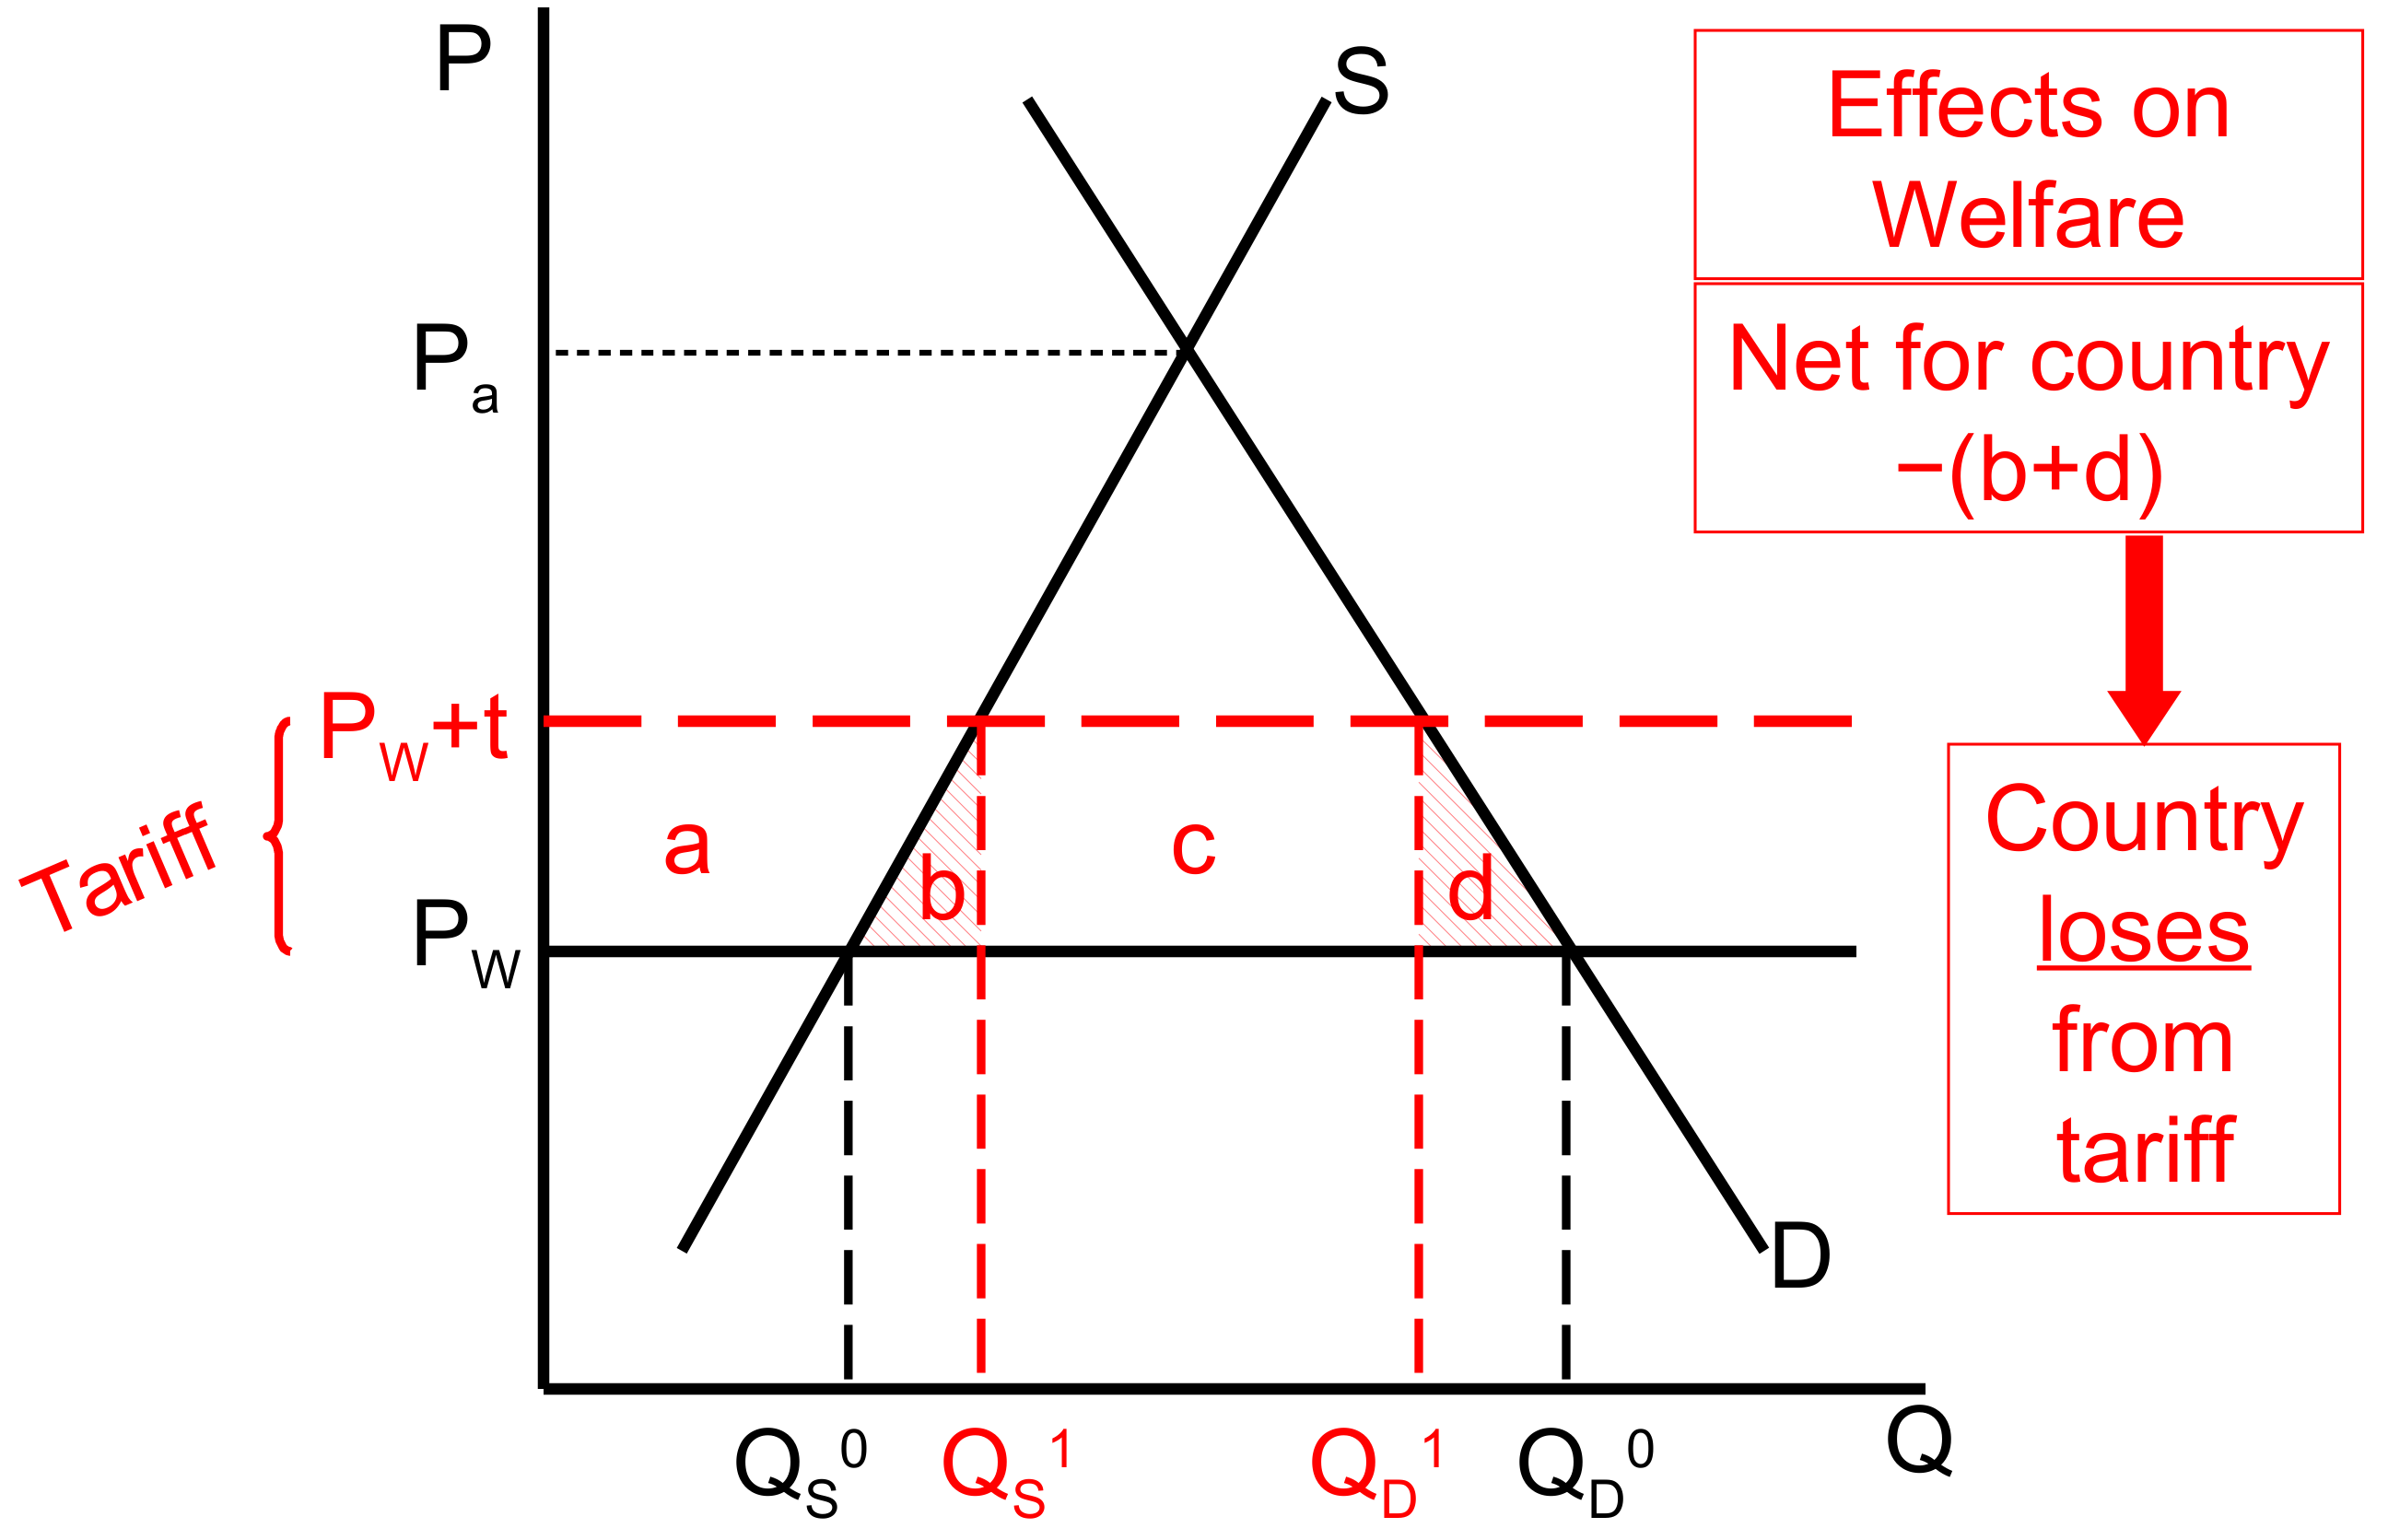
\includegraphics[scale=.5]{tariff_small_country7.png}
  \end{figure}
\end{frame}
%--------------------------------------

%--------------------------------------
\begin{frame}
  For a large economy imposing a tariff is a way to influence the Terms of Trade, a country can
  \begin{itemize}
    \item Manipulate exports prices relative to imports
    \item Increase national income at expense of trading partners
  \end{itemize}
  \medskip
  The reduction in imports will lead to a lower world price.
  Imposing a tariff will improve welfare as long as the ToT gains outweigh the distortion loss.
  \begin{itemize}
    \item A critical assumption is that there is no retaliation leading to a trade war
  \end{itemize}
\end{frame}
%--------------------------------------

%--------------------------------------
\begin{frame}
  \begin{figure}
    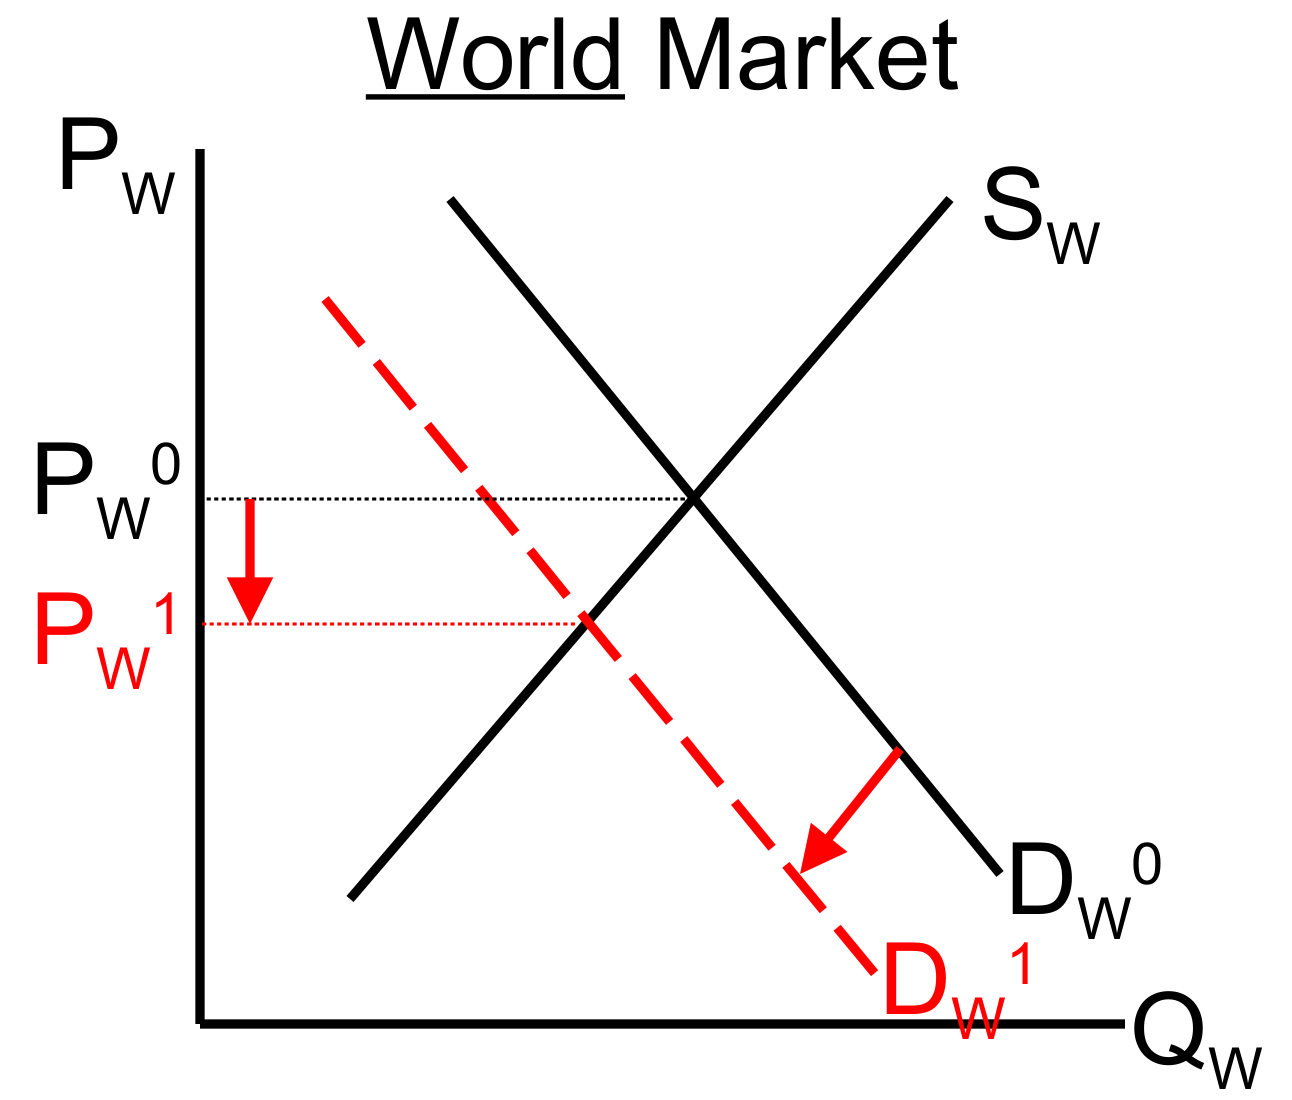
\includegraphics[scale=.5]{world_market.png}
  \end{figure}
\end{frame}
%--------------------------------------

%--------------------------------------
\begin{frame}
 Recall, Terms of Trade are calculated as 
 \begin{align*}
   ToT = \frac{p_x}{p_m}
 \end{align*}
 \medskip
 When the ToT increases welfare improves as the country can get more import in return for exports
 \begin{itemize}
   \item Large country can drive down world price of imports, improving ToT
 \end{itemize}
\end{frame}
%--------------------------------------

%--------------------------------------
\begin{frame}
 The possible gains from trade is sometimes also called the monopoly effect
 \begin{itemize}
   \item Monopolies increase profit by selling less at higher prices
 \end{itemize}
 \medskip
 A large country can increase welfare by
 \begin{itemize}
   \item Importing less, using a tariff, thereby reducing the price it pays
 \end{itemize}
 \medskip
 A large country can also gain by restricting exports
 \begin{itemize}
   \item e.g. OPEC and oil exports at times
 \end{itemize}
\end{frame}
%--------------------------------------

%--------------------------------------
\begin{frame}{Tariff effect in large country}
  \begin{figure}
    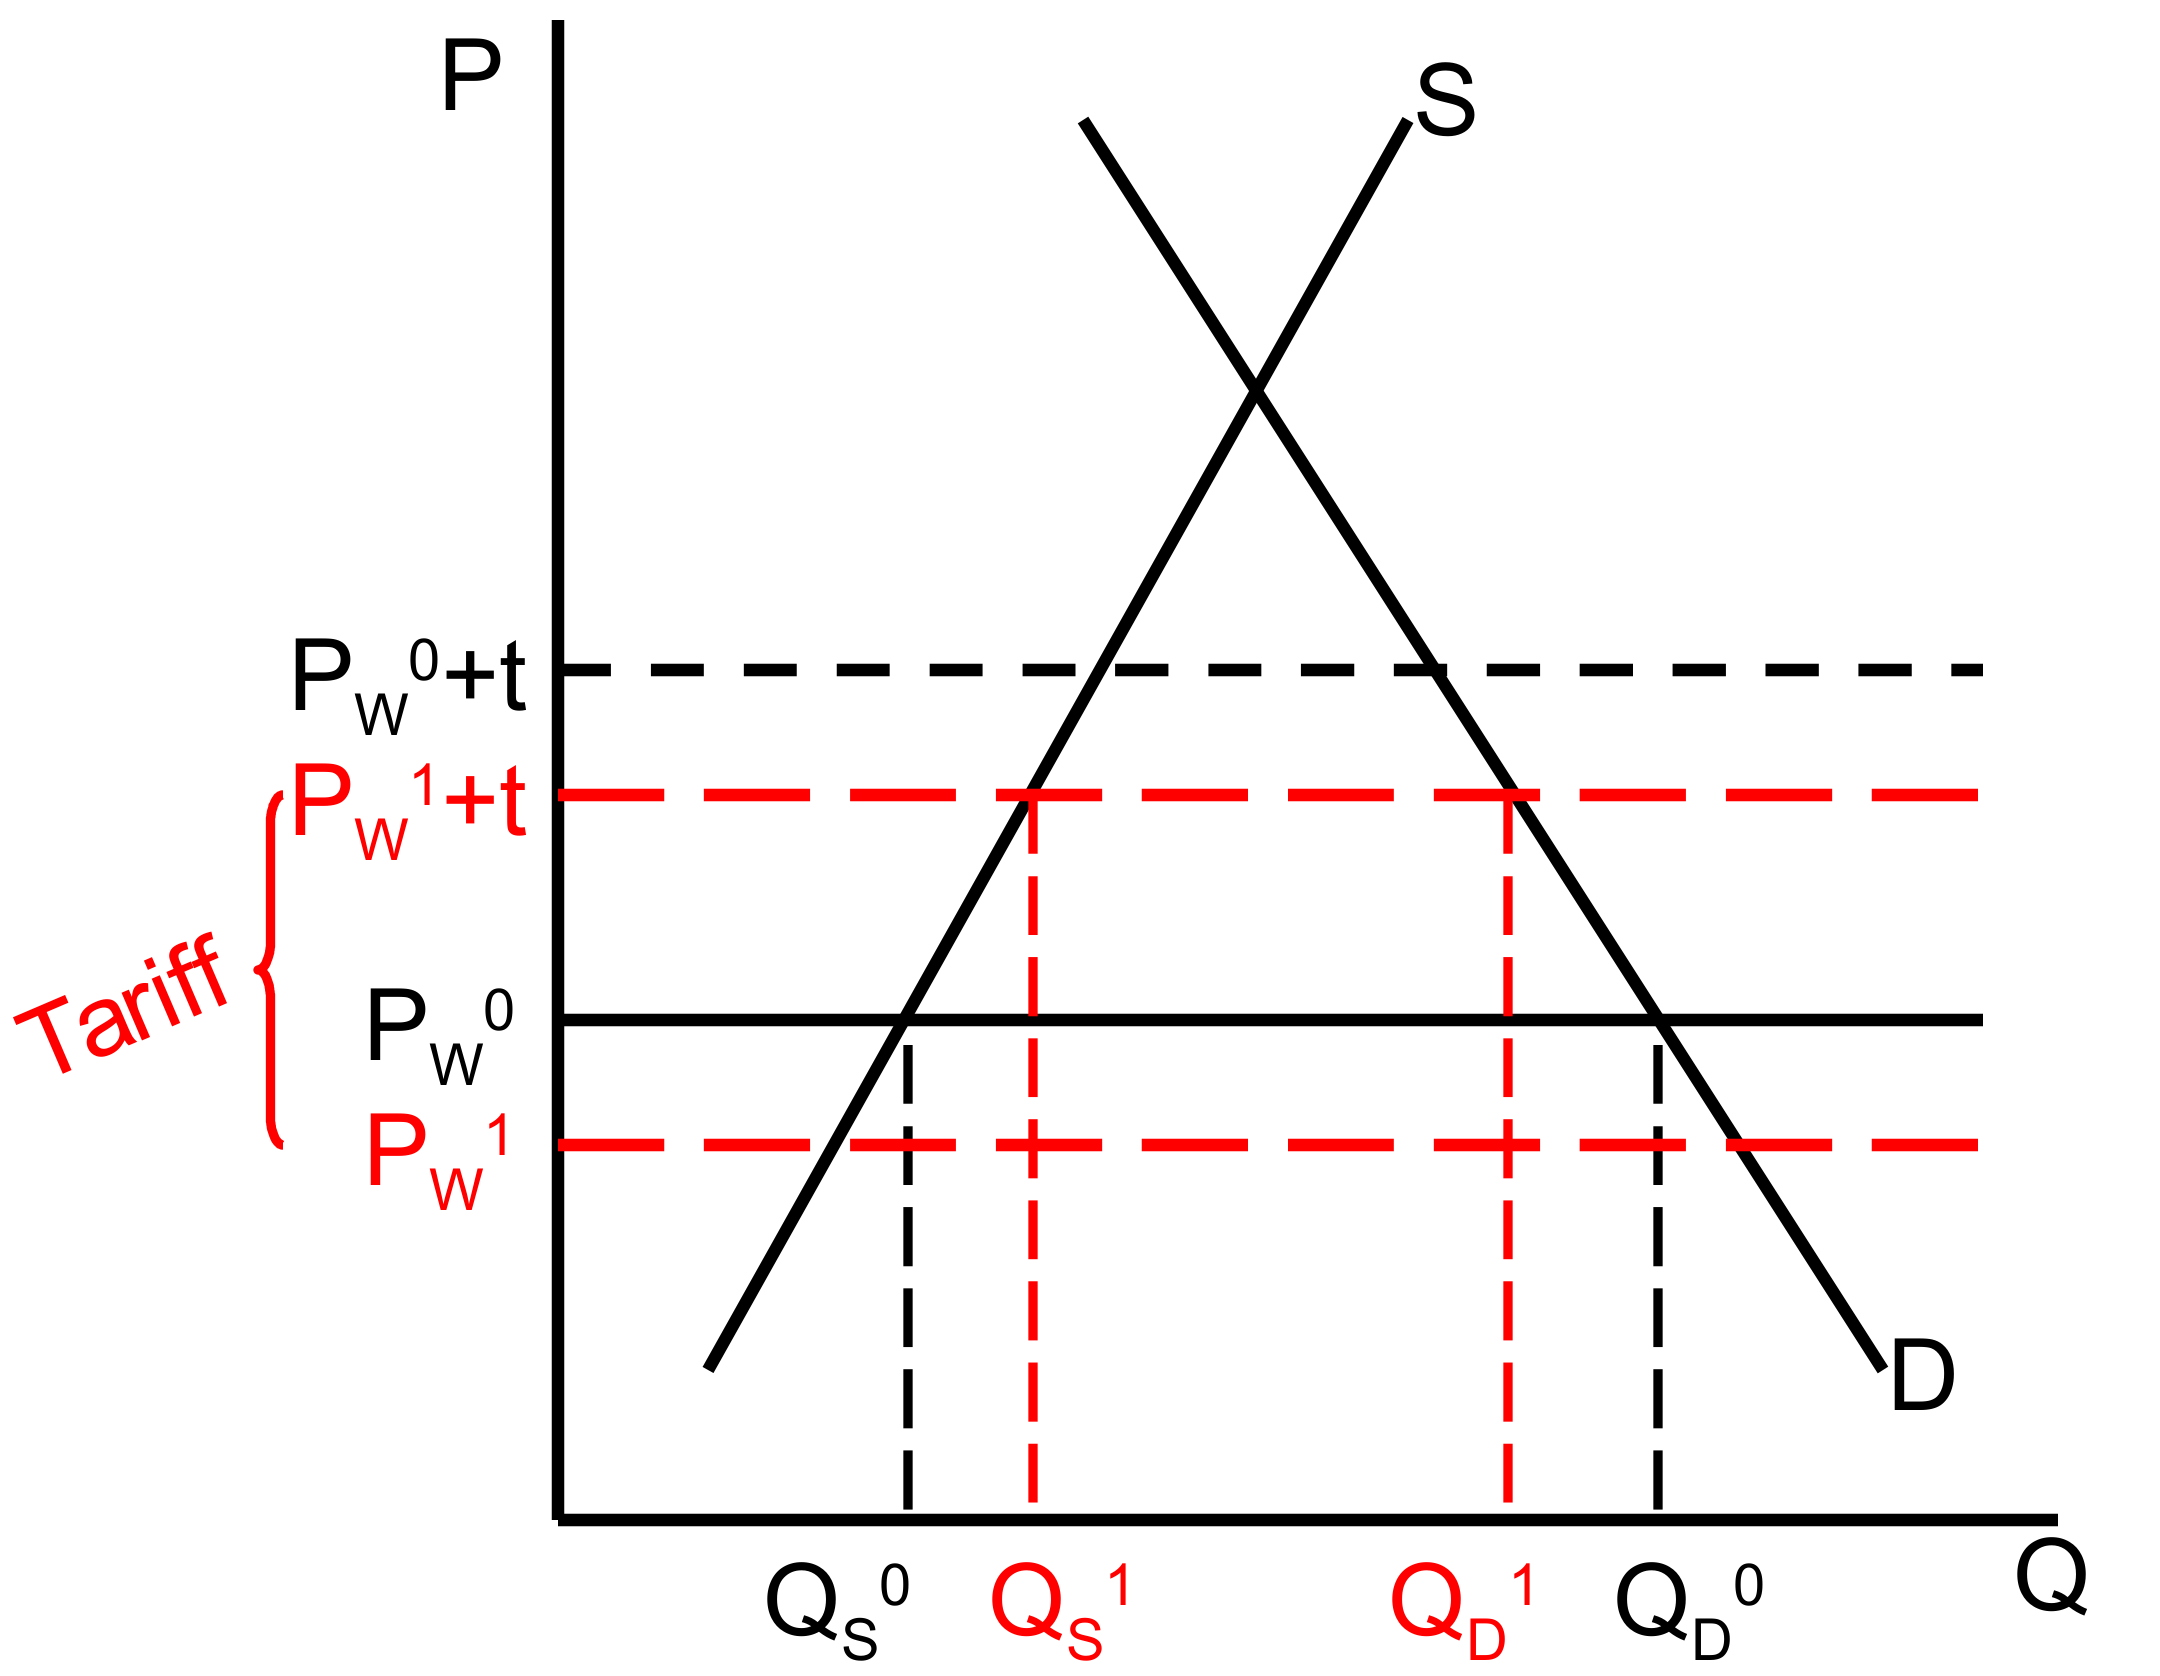
\includegraphics[scale=.5]{tariff_large_country1.png}
  \end{figure}
\end{frame}
%--------------------------------------

%--------------------------------------
\begin{frame}
  As a result of implementing the tariff AND the subsequent fall in world prices the domestic price will increase, but in comparison to a small economy  
  \begin{enumerate}
    \item Output will increase by less, making the producer surplus smaller
    \item Reduction in consumption is lower which means that consumer loss is smaller as well
  \end{enumerate}
  \medskip
  Since imports fall by less as well the tariff revenue is larger.
\end{frame}
%--------------------------------------

%--------------------------------------
\begin{frame}{Tariff effect in large country}
  \begin{figure}
    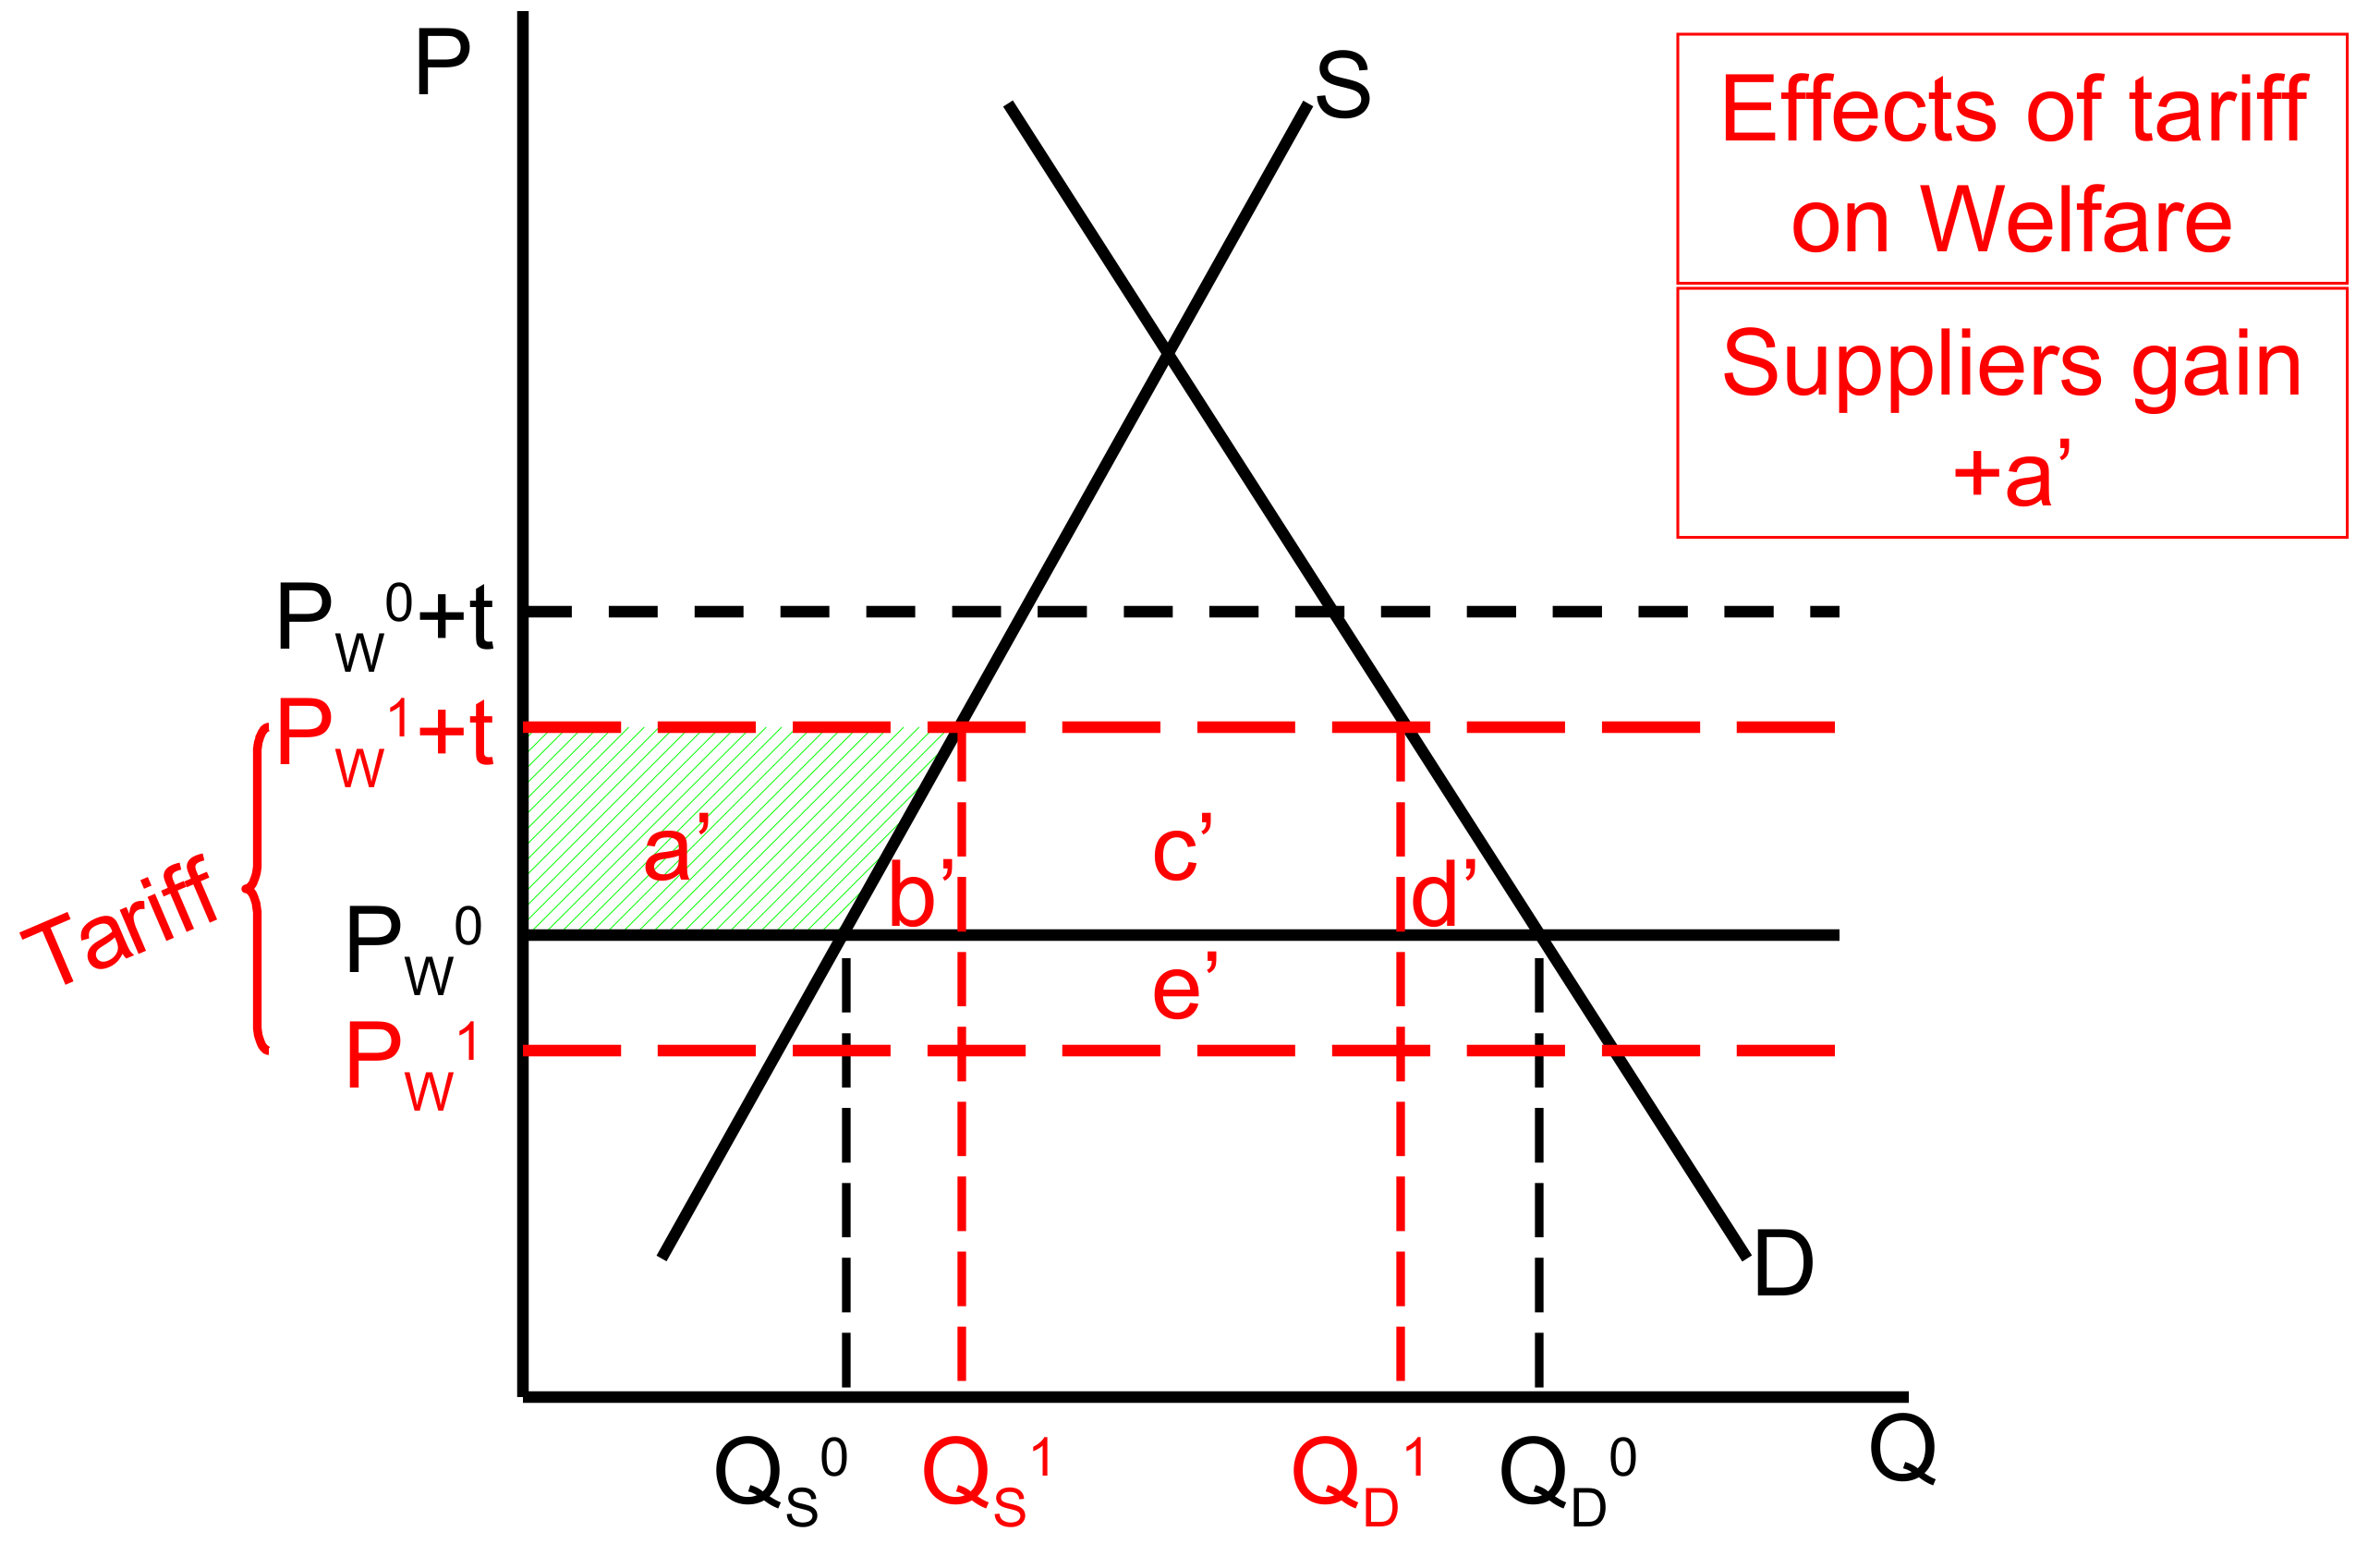
\includegraphics[scale=.5]{tariff_large_country2.png}
  \end{figure}
\end{frame}
%--------------------------------------

%--------------------------------------
\begin{frame}{Tariff effect in large country}
  \begin{figure}
    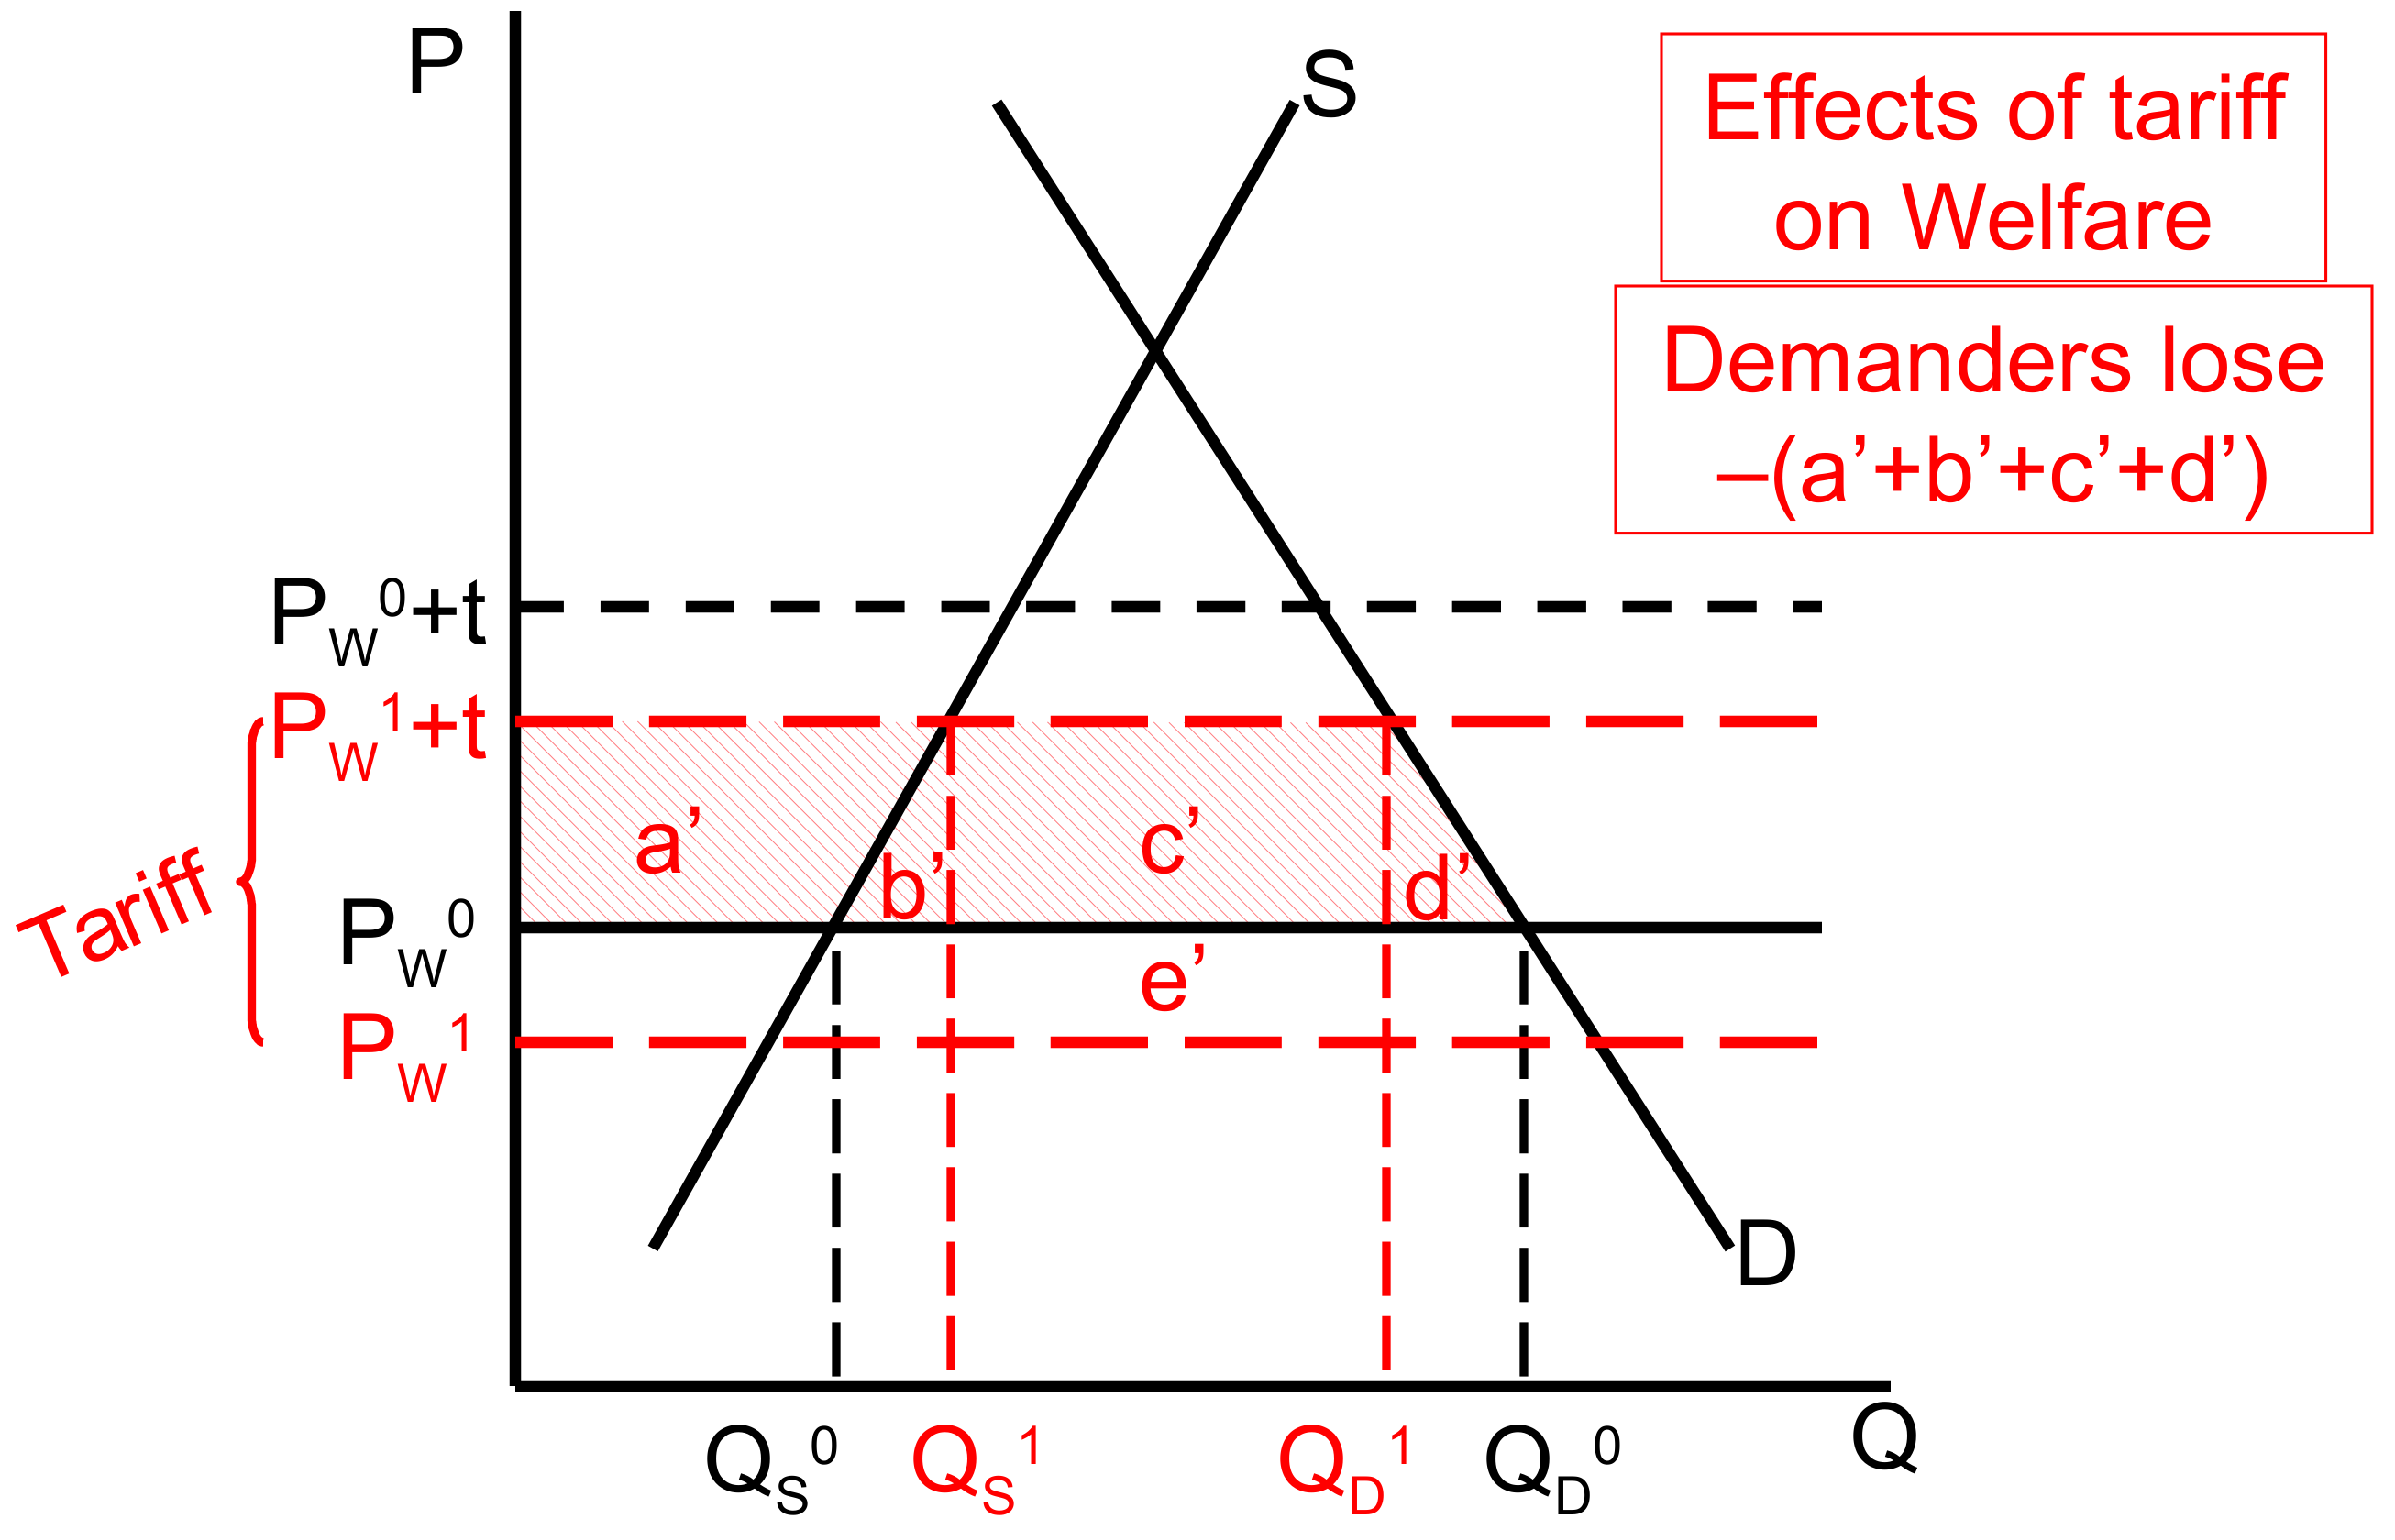
\includegraphics[scale=.5]{tariff_large_country3.png}
  \end{figure}
\end{frame}
%--------------------------------------

%--------------------------------------
\begin{frame}{Tariff effect in large country}
  \begin{figure}
    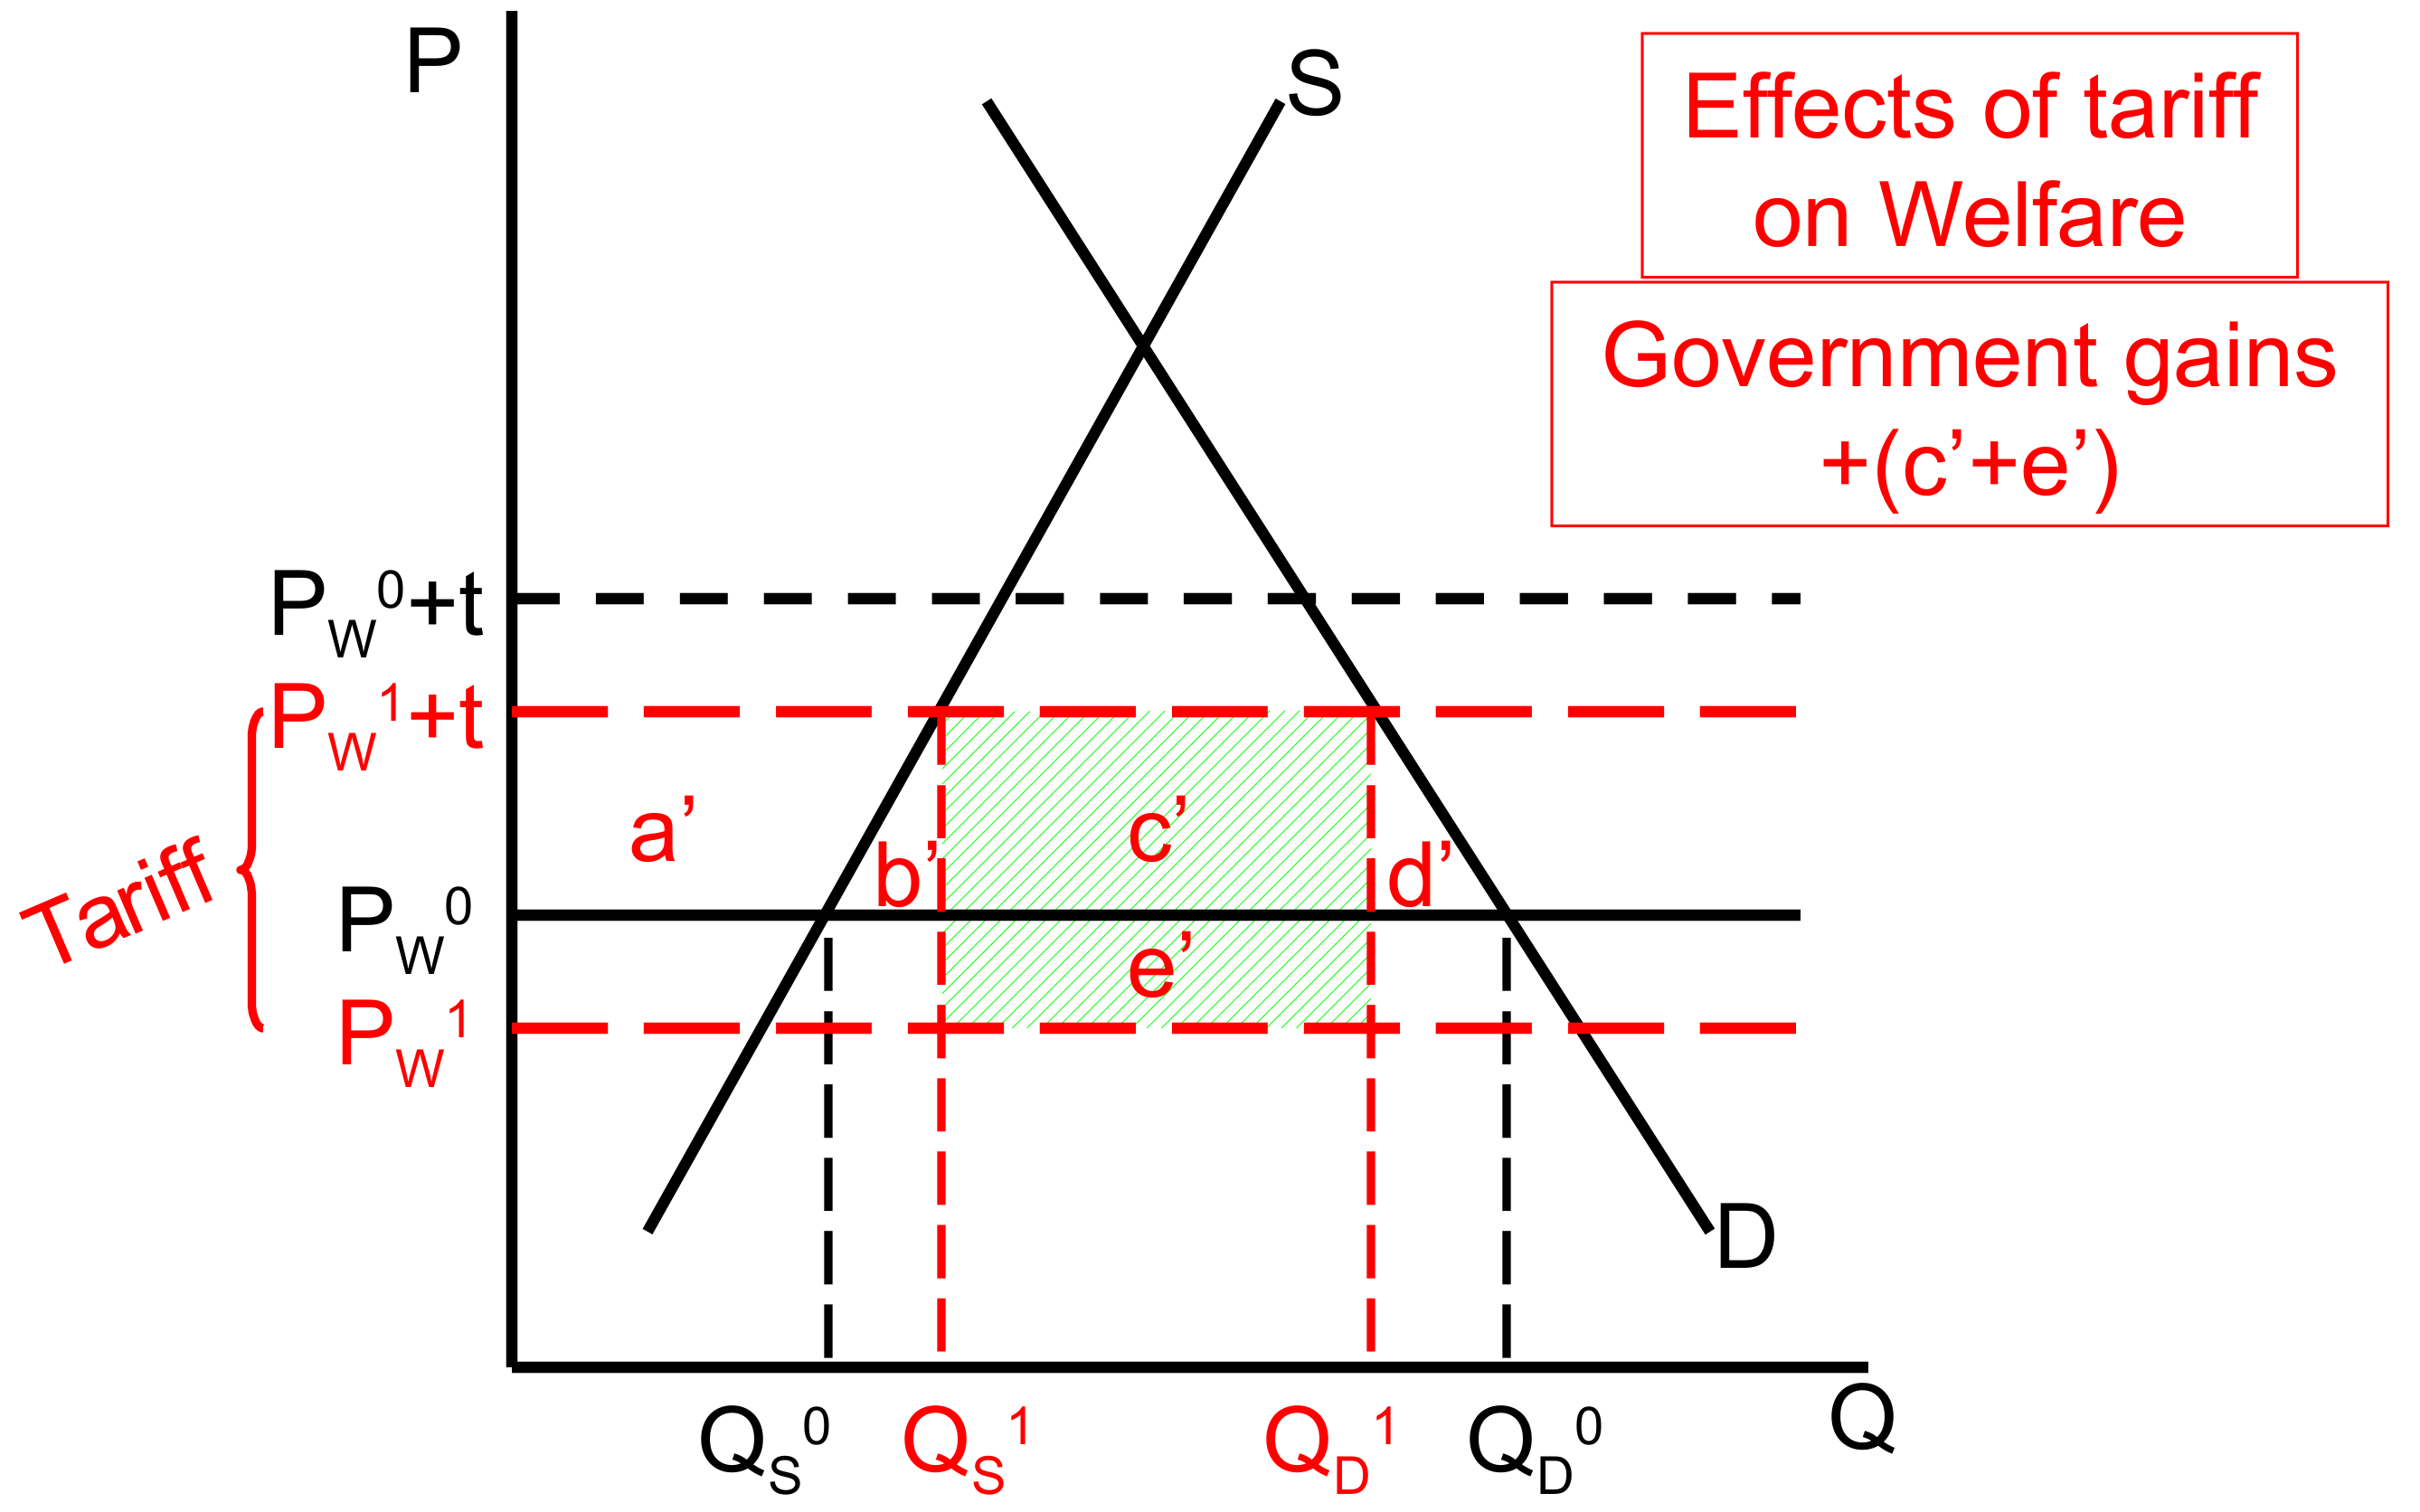
\includegraphics[scale=.5]{tariff_large_country4.png}
  \end{figure}
\end{frame}
%--------------------------------------

%--------------------------------------
\begin{frame}{Tariff effect in large country}
  \begin{figure}
    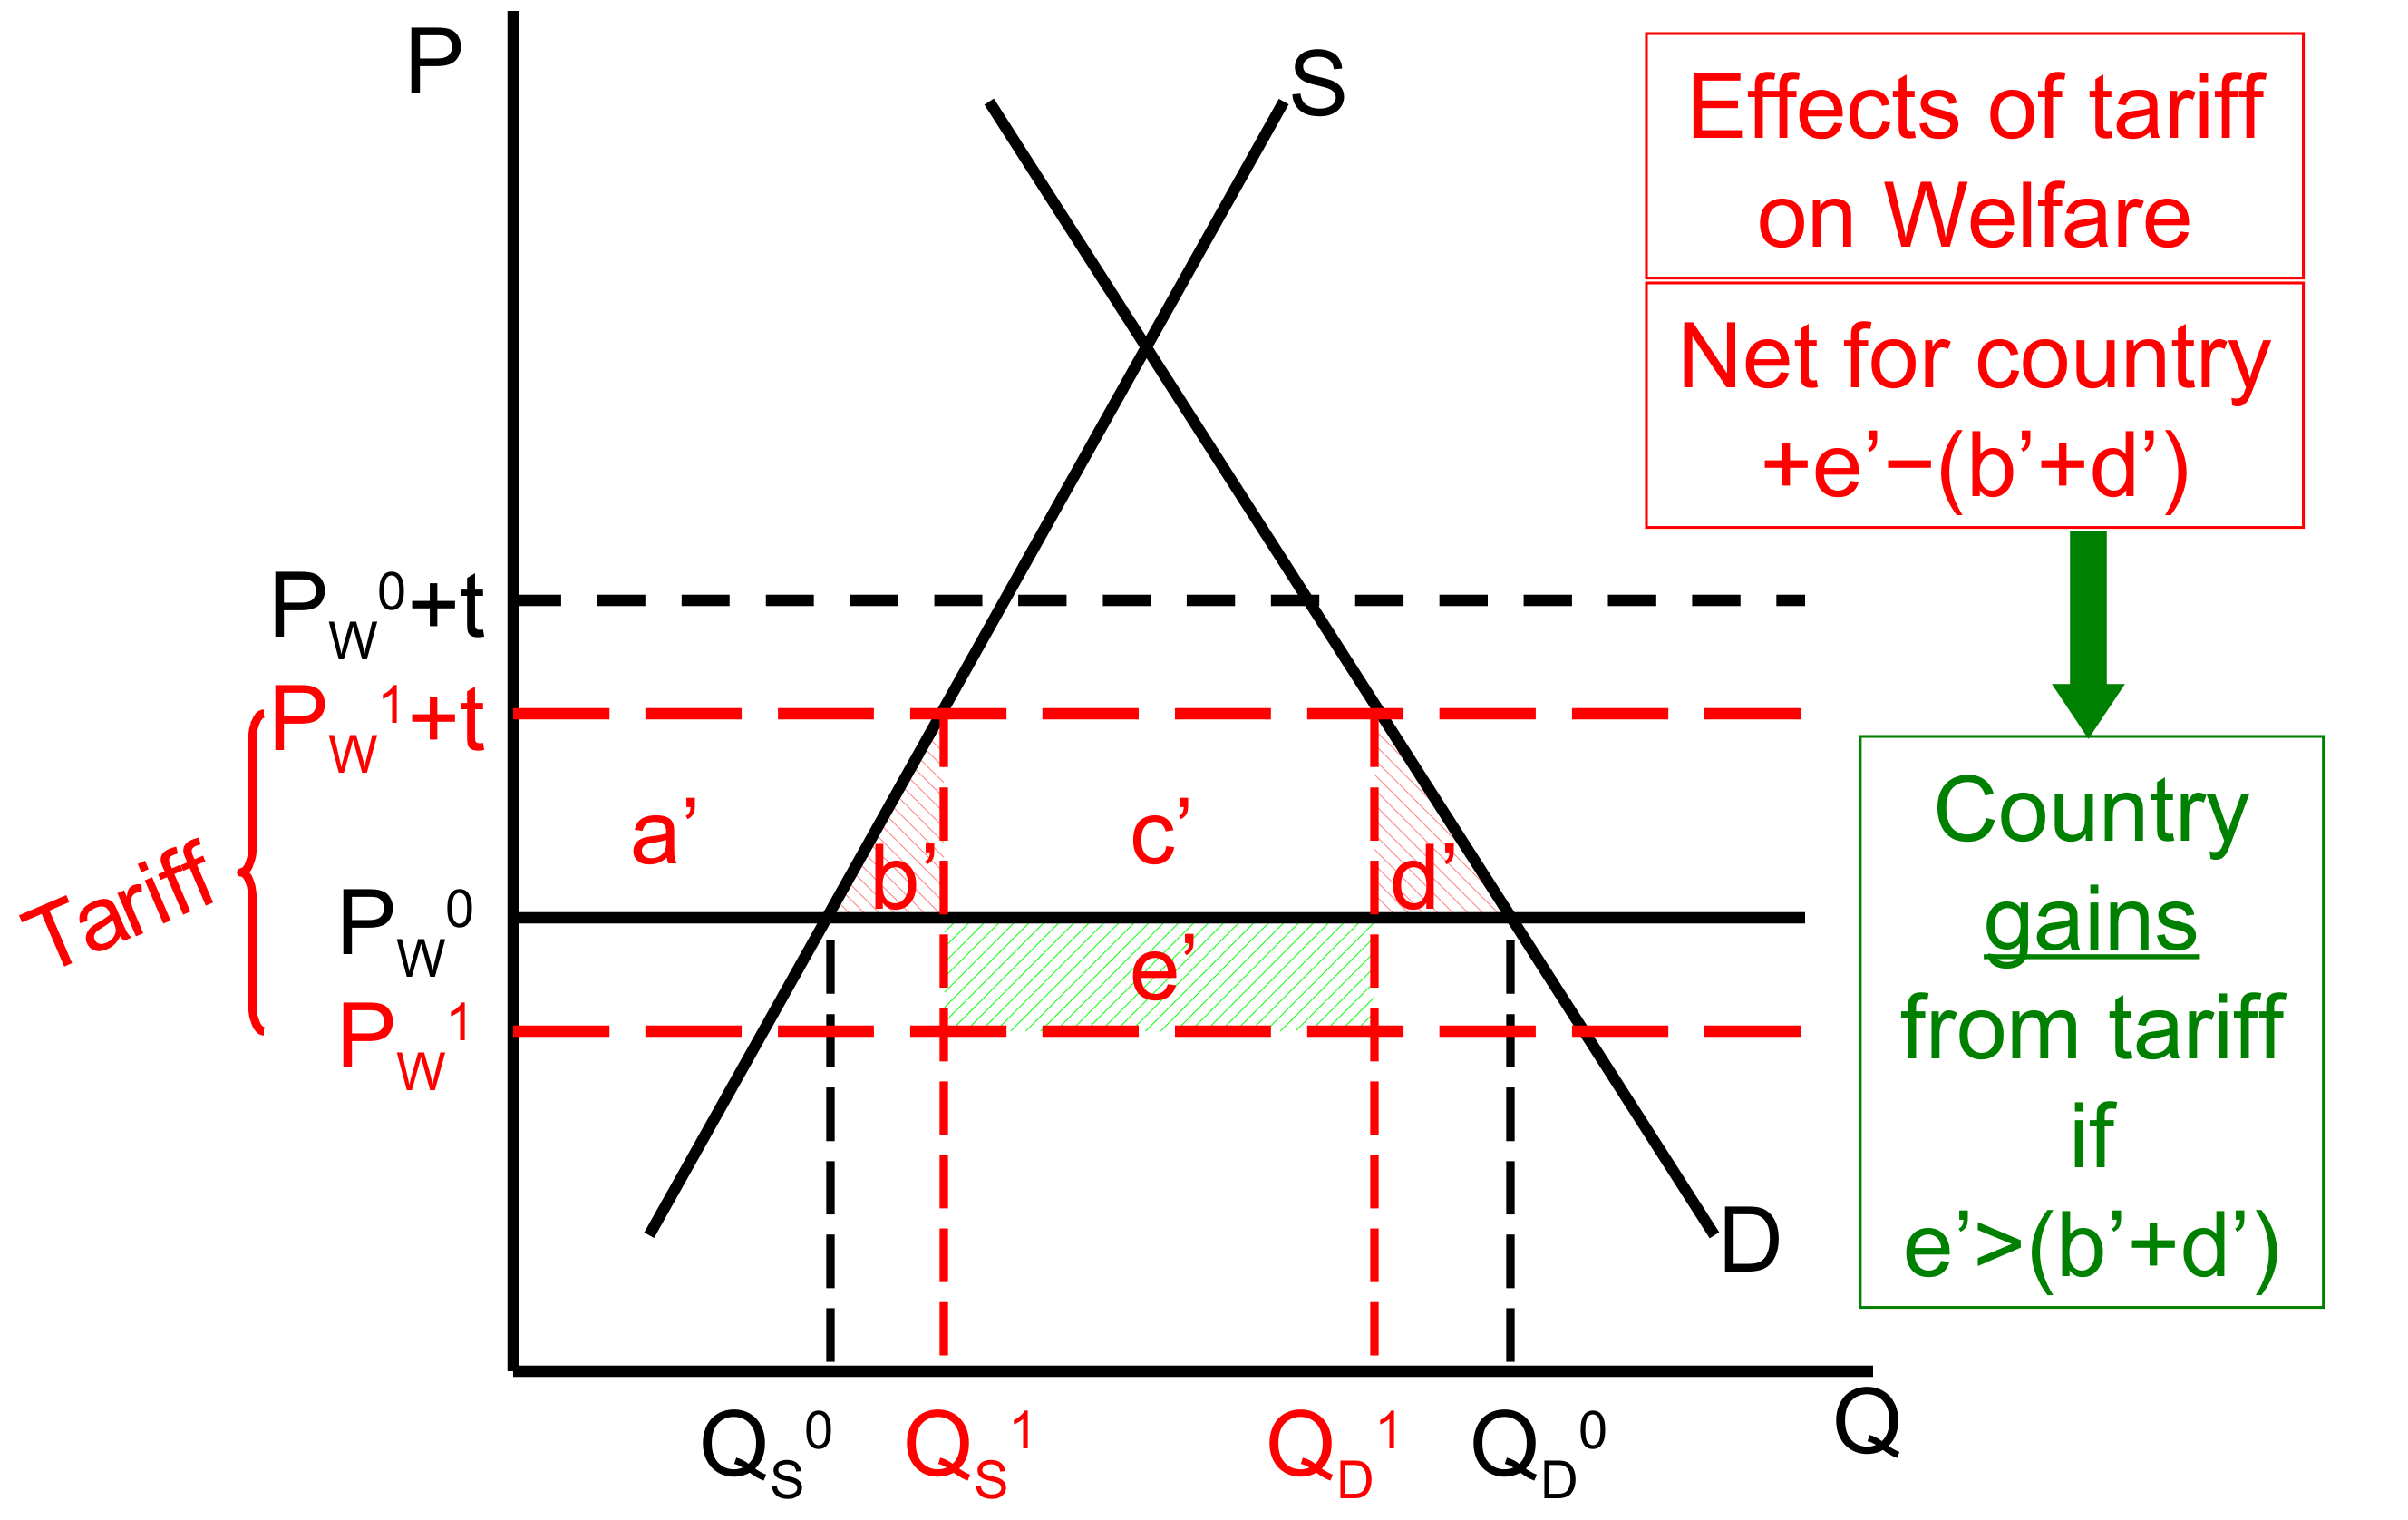
\includegraphics[scale=.5]{tariff_large_country5.png}
  \end{figure}
\end{frame}
%--------------------------------------

%--------------------------------------
\begin{frame}
  For a large country there is such thing as an optimal tariff
  \begin{itemize}
    \item If the tariff is too large it will lose
  \end{itemize}
  \begin{figure}
    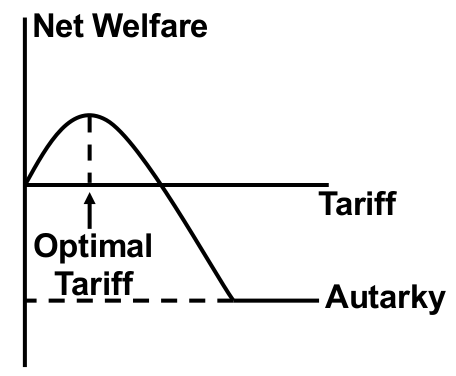
\includegraphics{optimal_tariff.png}
  \end{figure}
\end{frame}
%--------------------------------------

%--------------------------------------
\begin{frame}
 Although a large economy could gain imposing a tariff it will
 \begin{itemize}
   \item Harm the other countries
   \item Reduce world welfare as the rest of the world losses will be larger than the country's gains
 \end{itemize}
 \medskip
 And of course there is the possibility that other countries retaliate with their own tariffs making everyone worse off.
\end{frame}
%--------------------------------------

%--------------------------------------
\begin{frame}
  Examining the effect of a tariff we can look at the Effective Rate of Protection (EPR). 
  There is often a difference between the set tariff rate and the effective rate of protection since
  \begin{itemize}
    \item Tariffs will affect sectors other than the protected sector
    \item Tariffs causes indirect effects on the prices and value added for the protected sector
  \end{itemize}
\end{frame}
%--------------------------------------

%--------------------------------------
\begin{frame}
 The EPR accounts for the effect of tariffs on the inputs and outputs and provides a level of protection in a certain industry.
 \begin{align*}
   EPR= \frac{t_o - at_i}{1-a}
 \end{align*}
 Here $t_o$ is the ad valorem tariff on output and $t_i$ the ad valorem tariff on input. $a$ is the share of input value relative to output value.
\end{frame}
%--------------------------------------

%--------------------------------------
\begin{frame}
  Suppose that the world market price for a bicycle is \texteuro 800 while the inputs cost \texteuro 600
  \begin{itemize}
    \item This means that the value added equals \texteuro 200
  \end{itemize}
  Now to protect its infant industry a country decides to charge a 25\% tariff on imported bicycles
  \begin{itemize}
    \item This means that home producers can now charge \texteuro 1000 for their bicycles
  \end{itemize}
  The effective rate of protection for home bicycle producers is the change in value added or
  \begin{align*}
    \frac{400-200}{200}=100\%
  \end{align*}
  Which is greater than the tariff rate
\end{frame}
%--------------------------------------

%--------------------------------------
\begin{frame}
  Now instead of a tariff on bicycles the country imposes a 10\% tariff on bicycle parts instead, in order to encourage domestic production. 
  As a result input costs increase from \texteuro 600 to \texteuro 660.\\
  \medskip
  This policy is less advantageous to bicycle assembly or home production of bicycles\footnote{Assuming price final product doesn't change!}
  \begin{itemize}
    \item Before: local assembly was worth \texteuro 200
    \item After: local assembly is worth \texteuro 140
  \end{itemize}
  The new tariff only protects producers of bicycle parts, but not bicycle producers:
  \begin{align*}
    \frac{140-200}{200}=-30\%
  \end{align*}  
\end{frame}
%--------------------------------------

%--------------------------------------
\begin{frame}
 Besides tariffs there are other policy tools known as Non-Tariff Barriers (NTBs).
 An NTB is
 \begin{quote}
 Any institutional or policy arrangement that interferes with trade AND is not a tariff.
 \end{quote}
 \medskip
 Term is also used for policies that expand trade. 
\end{frame}
%--------------------------------------

%--------------------------------------
\begin{frame}
  Main types of NTB are
  \begin{enumerate}
    \item Import quotas
    \item Export subsidies    
    \item Voluntary export restraints (VER)
    \medskip
    \item Embargo
    \item Indirect tariff measures, e.g. health and safety standards
  \end{enumerate}
  \medskip  
  Compared to tariffs these are all worse options given that there is no increase in government revenue associated with them.  
\end{frame}
%--------------------------------------

%--------------------------------------
\begin{frame}
  An import quota restricts the quantity of a particular good that may be imported and is enforced by
  \begin{itemize}
    \item Licences
    \item Quota rights
  \end{itemize}
  A binding import quota will increase import prices because the quantity demanded will exceed the quantity supplied both by domestic producers and imports.  
\end{frame}
%--------------------------------------

%--------------------------------------
\begin{frame}{US domestic and world sugar prices}
  \begin{figure}
    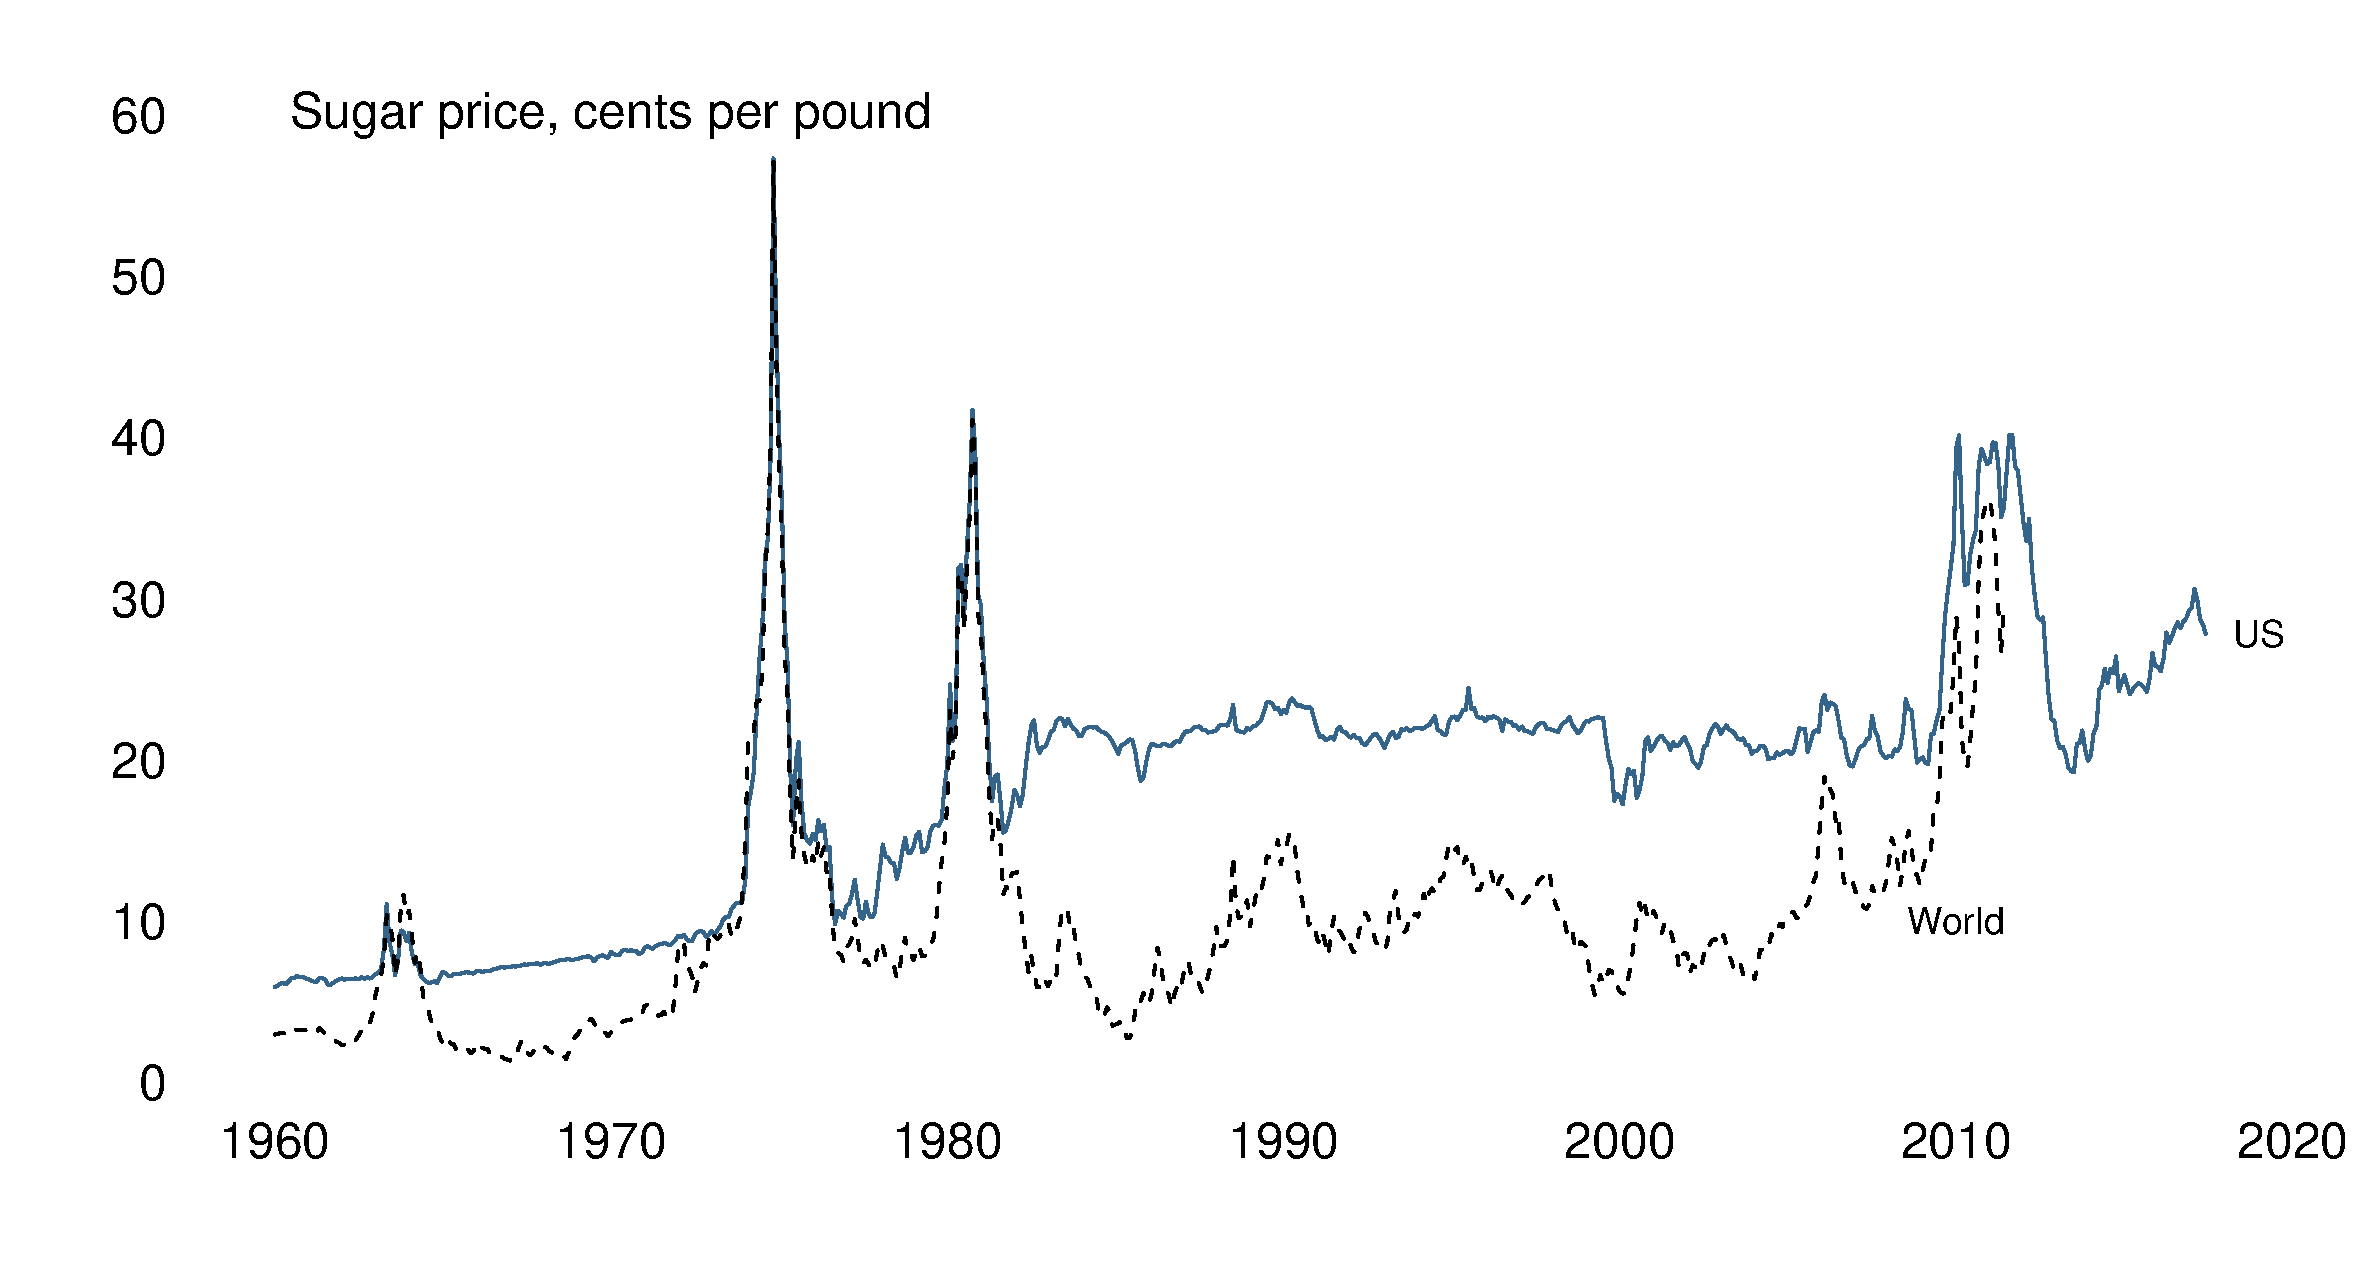
\includegraphics[scale=.25]{sugar_price}
  \end{figure}
\end{frame}
%--------------------------------------

%--------------------------------------
\begin{frame}
 The USA guarantees domestic sugar producers a break-even price
 \begin{itemize}
   \item Meaning that the USDA will buy any amount of sugar at this price
 \end{itemize}
  \medskip
  Even with this break-even price the domestic production is not enough to satisfy demand, which means that they have to import from the world market, which they do imposing import quotas
  \begin{itemize}
     \item They let foreign governments administer the quota and retain the quota rents
     \item Quota equals 1.4m tonnes annually
   \end{itemize} 
   \medskip
   As a result of this trade policy the price of sugar has been about twice as large as the world market price. 
\end{frame}
%--------------------------------------

%--------------------------------------
\begin{frame}{Effect of US sugar import quota}
  \begin{figure}
    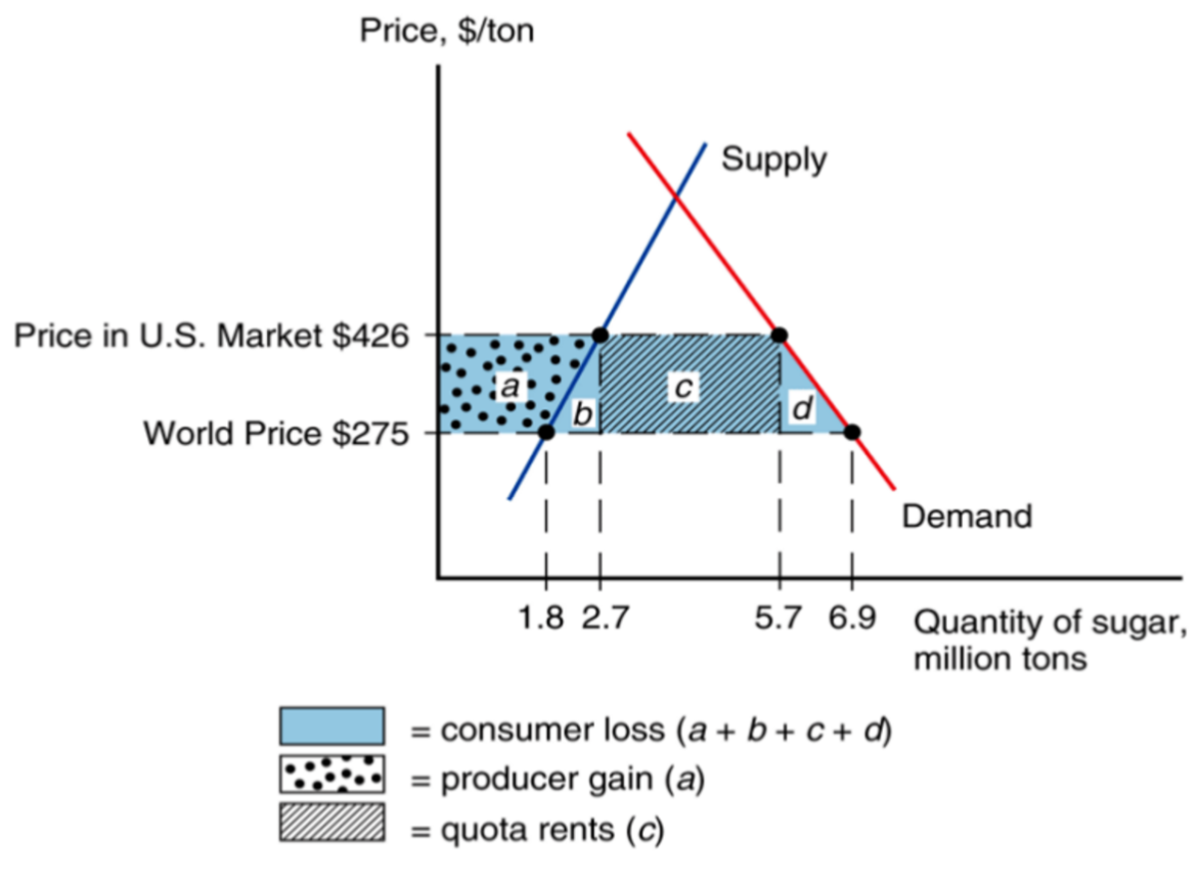
\includegraphics{sugar_quota}
  \end{figure}
\end{frame}
%--------------------------------------

%--------------------------------------
\begin{frame}{US obesity prevalence}
  \begin{figure}
    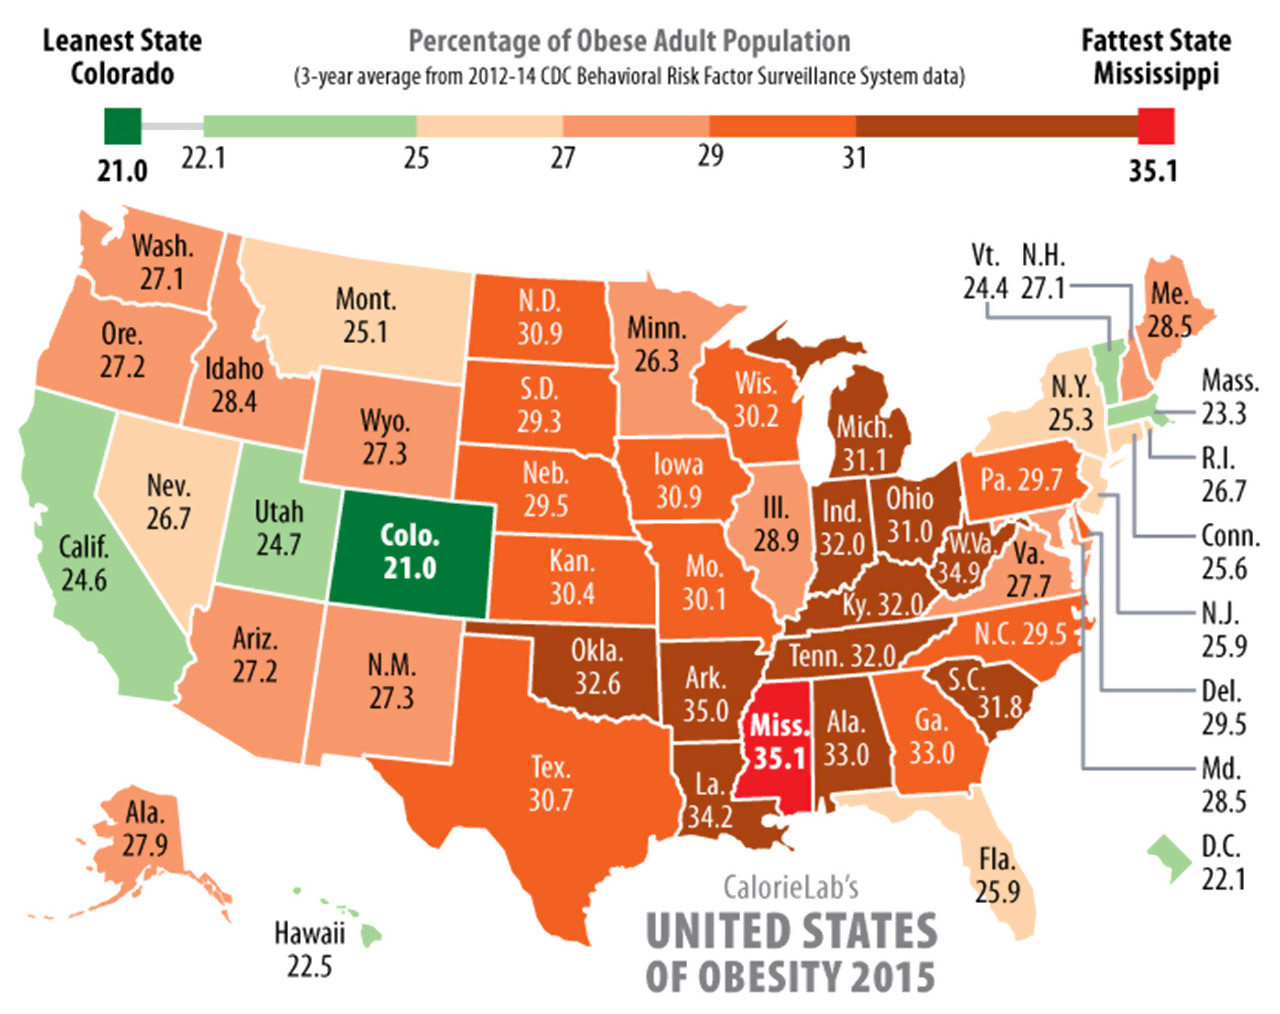
\includegraphics[scale=.2]{obesity}
  \end{figure}
\end{frame}
%--------------------------------------

%--------------------------------------
\begin{frame}
  Unlike a tariff a quota becomes more restrictive when
  \begin{itemize}
    \item Foreign supply increases
    \item World prices drop
  \end{itemize}
\end{frame}
%--------------------------------------

%--------------------------------------
\begin{frame}
  \begin{figure}
    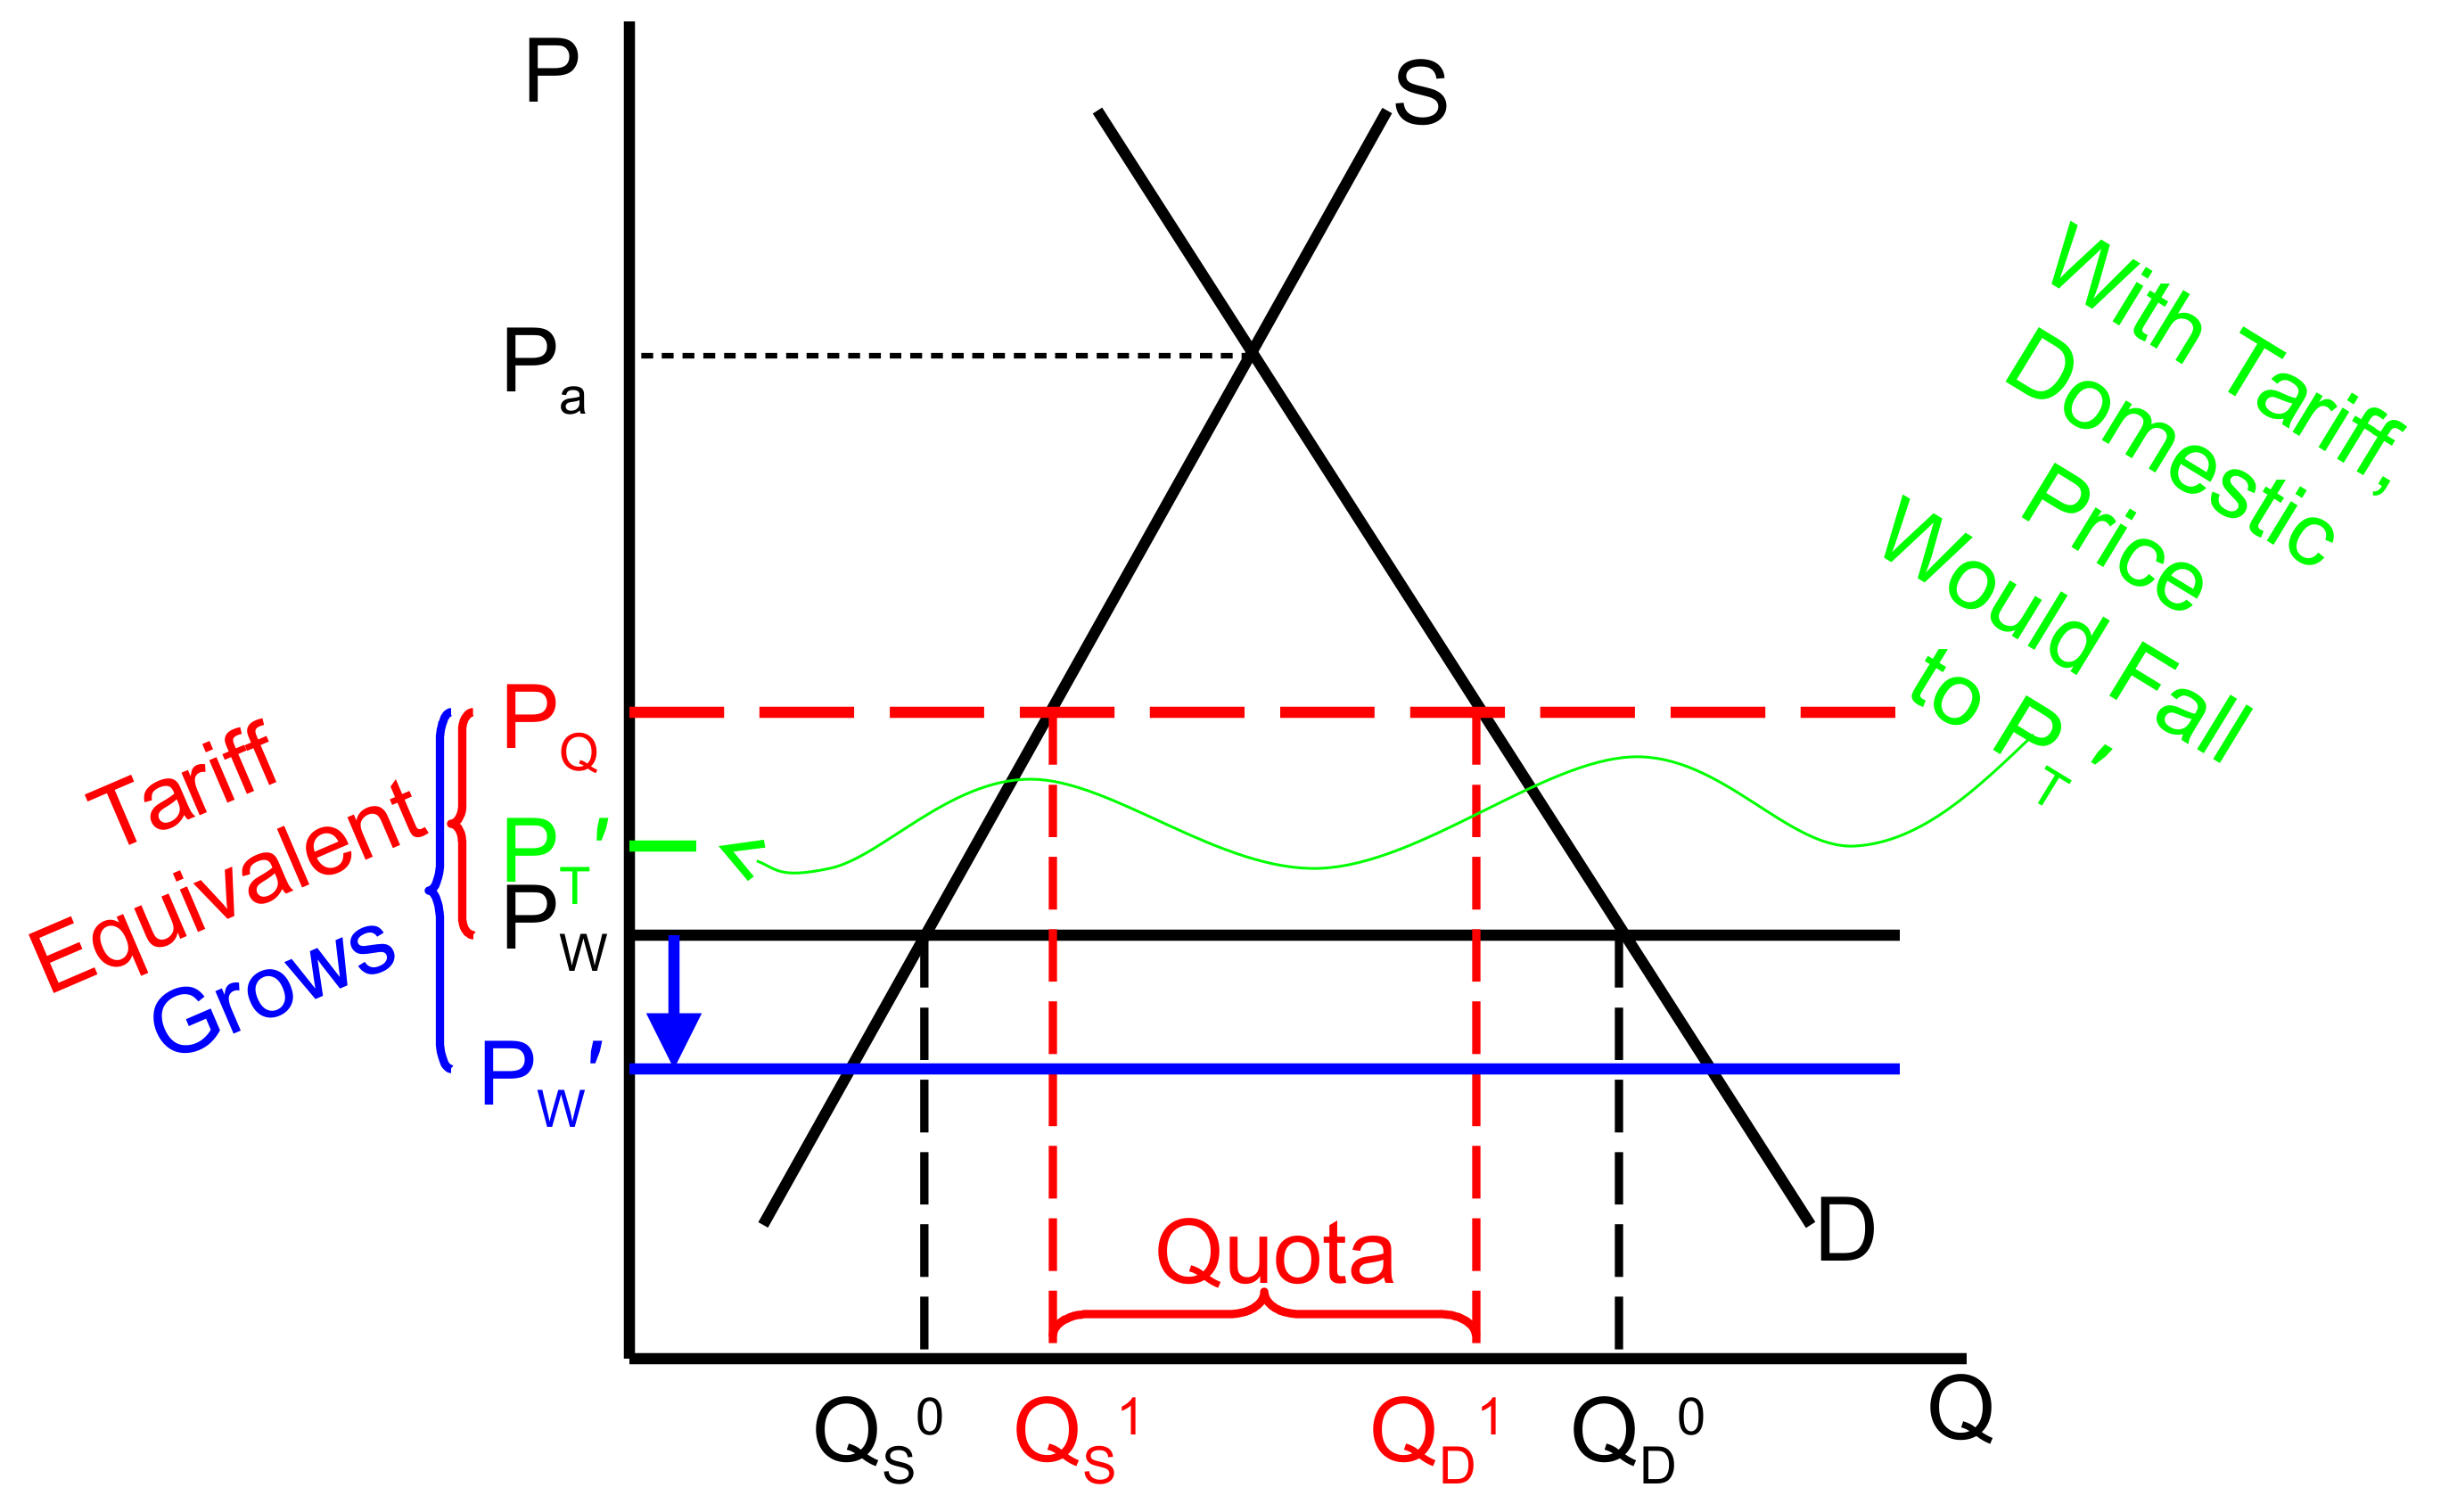
\includegraphics[scale=.5]{price_drop.png}
  \end{figure}
\end{frame}
%--------------------------------------

%--------------------------------------
\begin{frame}
 Following a decrease in world prices the tariff equivalent of the quote increases as well as the quote rents. 
 What doesn't change are
 \begin{itemize}
   \item Domestic price
   \item Domestic production and consumption
   \item Imports   
 \end{itemize}
 \end{frame}
%--------------------------------------

%--------------------------------------
\begin{frame}
  \begin{figure}
    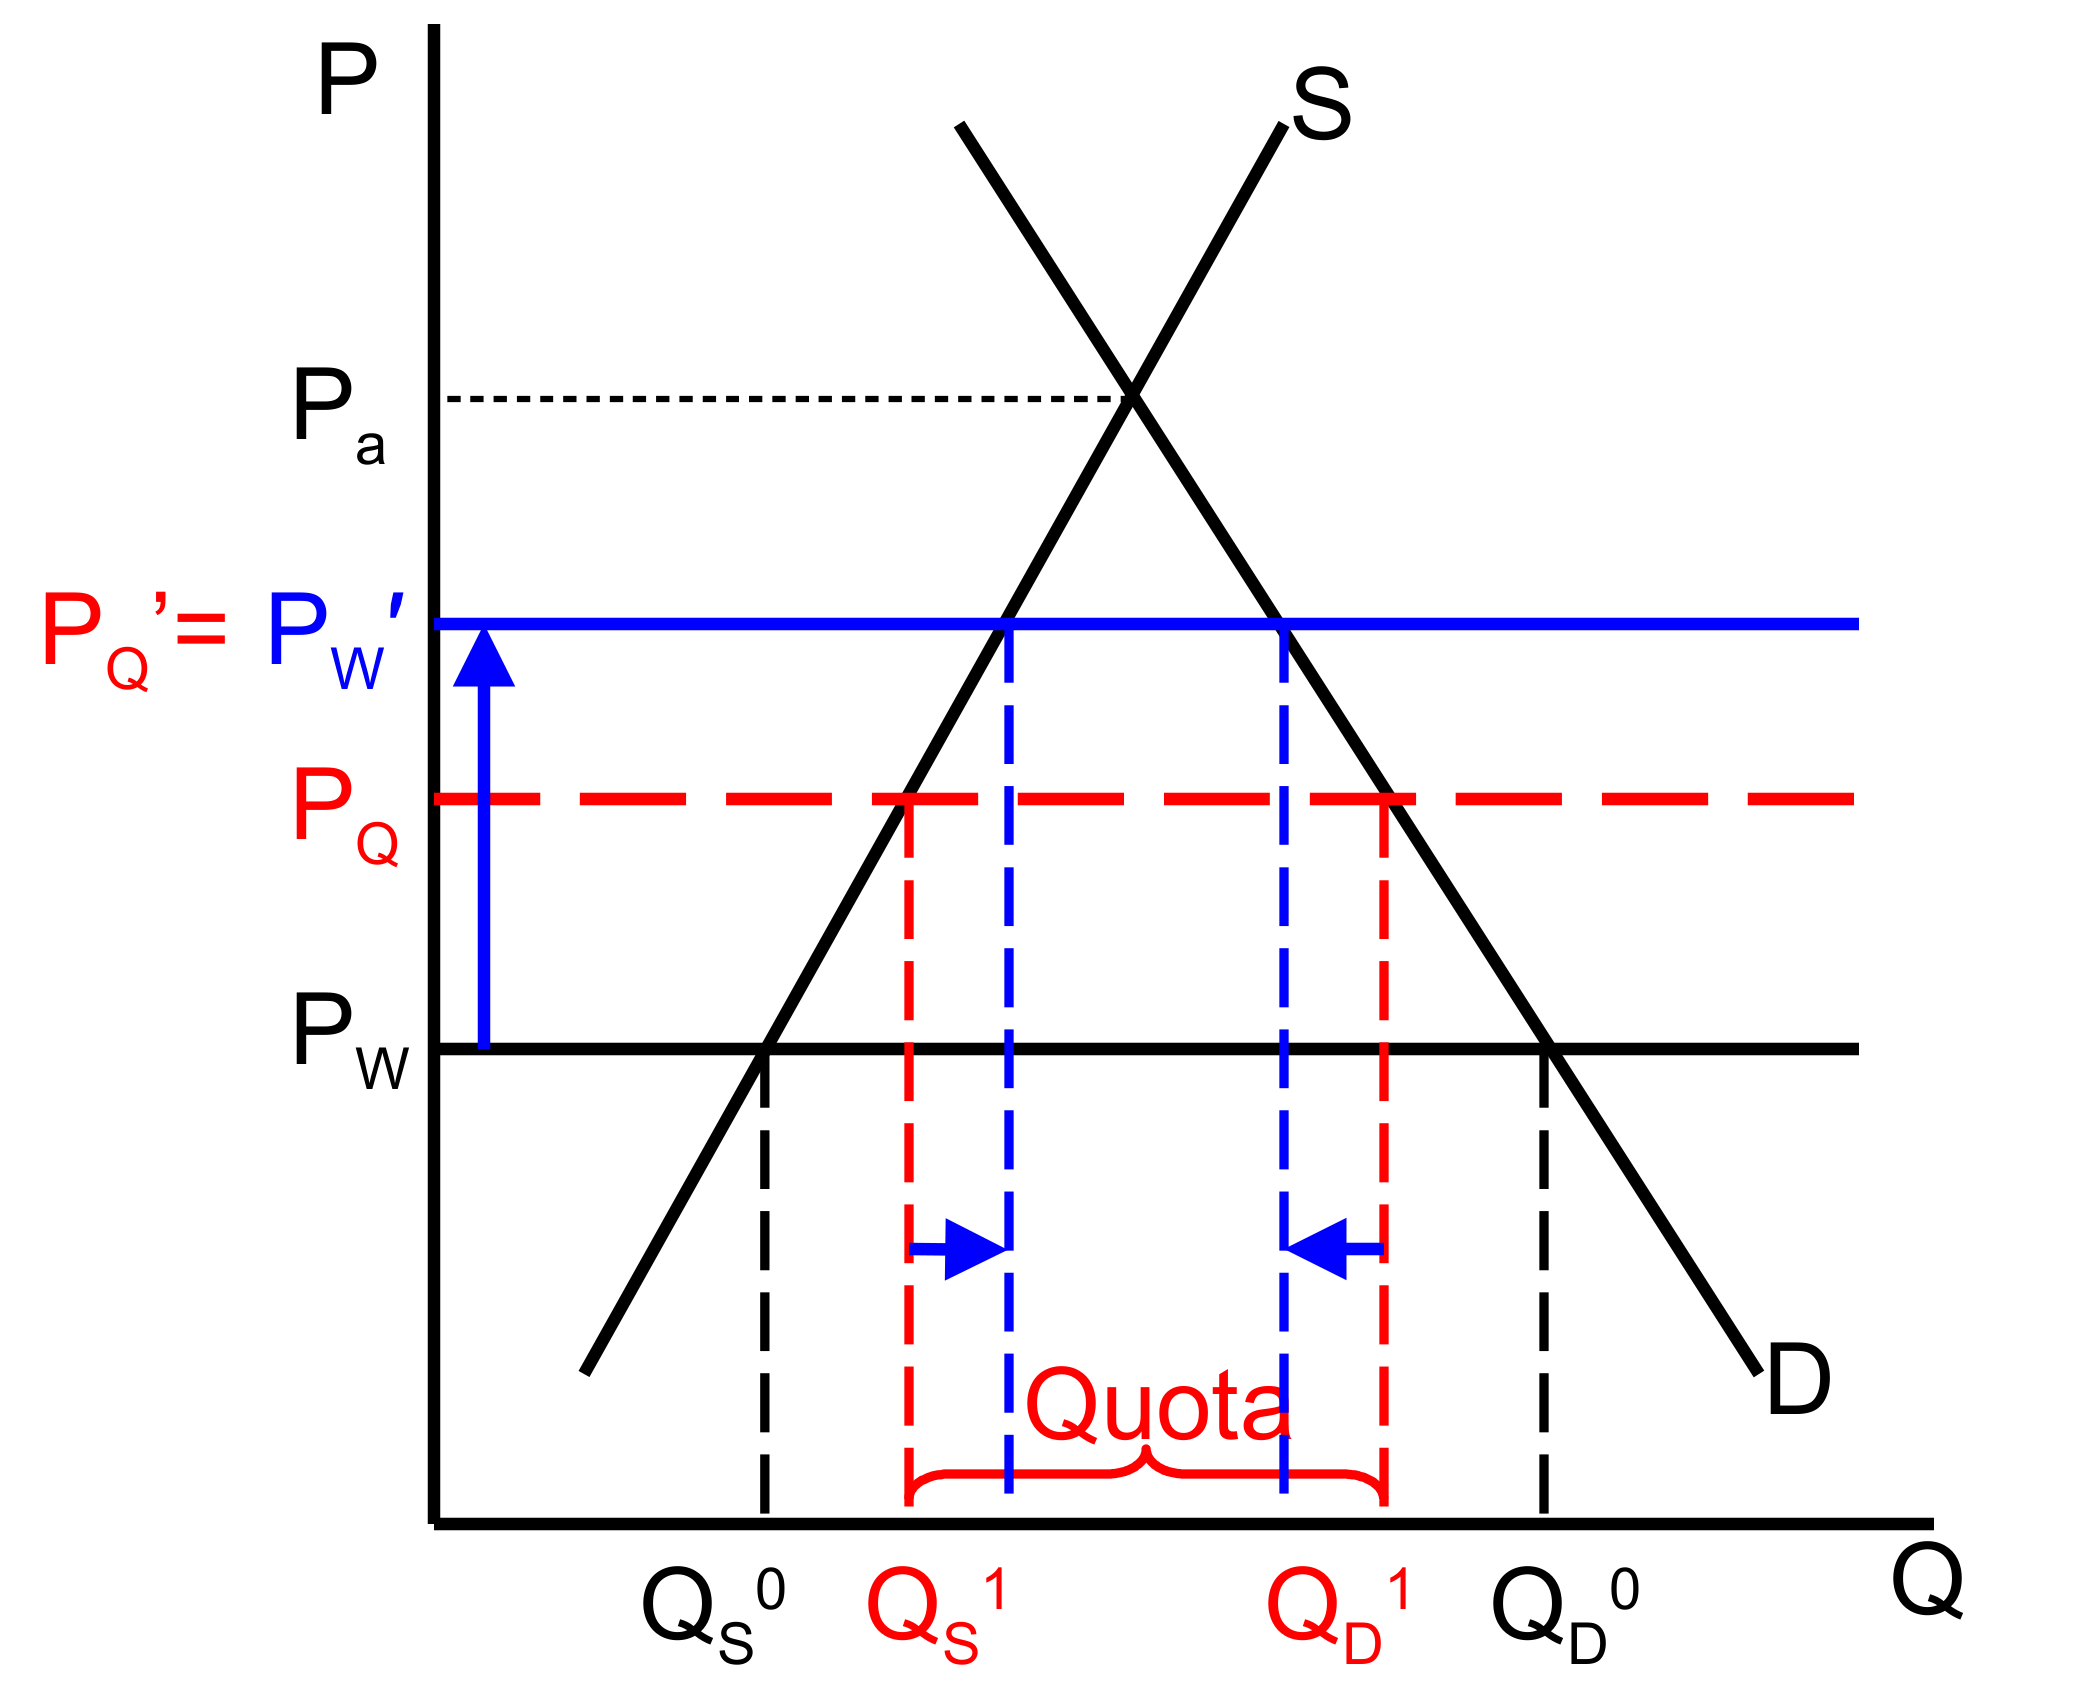
\includegraphics[scale=.5]{price_increase.png}
  \end{figure}
\end{frame}
%--------------------------------------

%--------------------------------------
\begin{frame}
 If prices increase the reverse will happen, if the increase is small, but for a large enough increase
 \begin{itemize}
   \item The quota is no longer binding and tariff equivalent becomes zero
   \item Domestic price will become world price
 \end{itemize}
 \medskip
 This is what happened to the US sugar price.
\end{frame}
%--------------------------------------

%--------------------------------------
\begin{frame}
 Importantly, quota rents go to the license holder. 
 Who holds the license? That depends on how it is administered
 \begin{enumerate}
   \item Auction licenses
   \item Distribute on first-come, first-served basis
   \item Give away to domestic firm
   \item Give away to foreign firm/government   
 \end{enumerate}
 \medskip
 Often licenses are distributed following approach 4 based on historical exports.
\end{frame}
%--------------------------------------

%--------------------------------------
\begin{frame}
  Like tariffs export subsidies can be ad valorem or specific.
  But they are the exact opposite of tariffs as the government pays producers to export
  \begin{figure}
    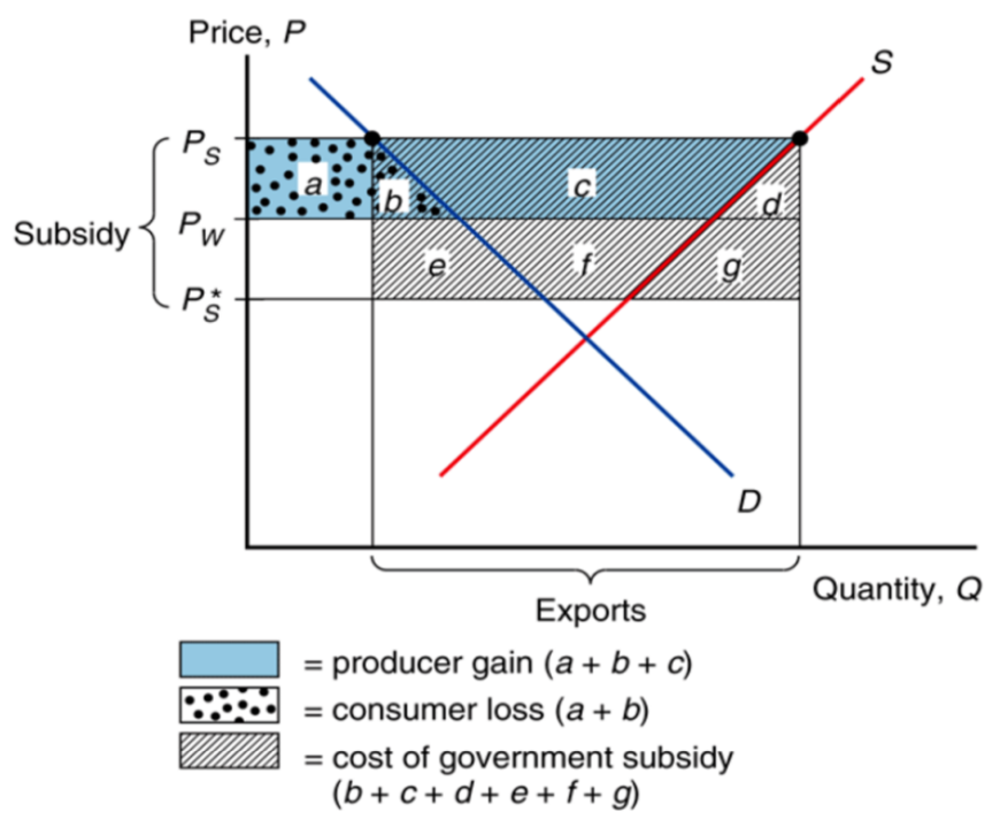
\includegraphics[scale=.7]{export_subsidy}
  \end{figure}
\end{frame}
%--------------------------------------

%--------------------------------------
\begin{frame}
  An export subsidy will increase the price in an exporting country
  \begin{itemize}
    \item Consumer surplus decreases, producer surplus increases
  \end{itemize}
  \medskip
  While government revenues will decrease
  \begin{itemize}
    \item Due to paying $sX^*$
  \end{itemize}
  Consumers in importing countries will benefit since they will pay
  \begin{align*}
  p^*=p_s-s
  \end{align*}   
  \medskip
  In contrast with a tariff the ToT will be worsened by export subsidies by lowering world market export prices.
\end{frame}
%--------------------------------------

%--------------------------------------
\begin{frame}
  The EU has the Common Agricultural Policy which is a system of agricultural subsidies in effect since 1962.
  The objective was to increase productivity and secure food supply at reasonable prices
  \begin{itemize}
    \item Turned the EU from food importer to net food exporter
  \end{itemize}
  \medskip
  The objectives of the programme seem to be out of date, but getting rid of the programme is difficult.
  Currently the programme is a big waste of tax money
  \begin{itemize}
    \item Accounts for 40\% of EU budget
    \item Costs roughly 30B EUR more than benefits
  \end{itemize}
\end{frame}
%--------------------------------------

%--------------------------------------
\begin{frame}{Effect of CAP on prices}
  \begin{figure}
    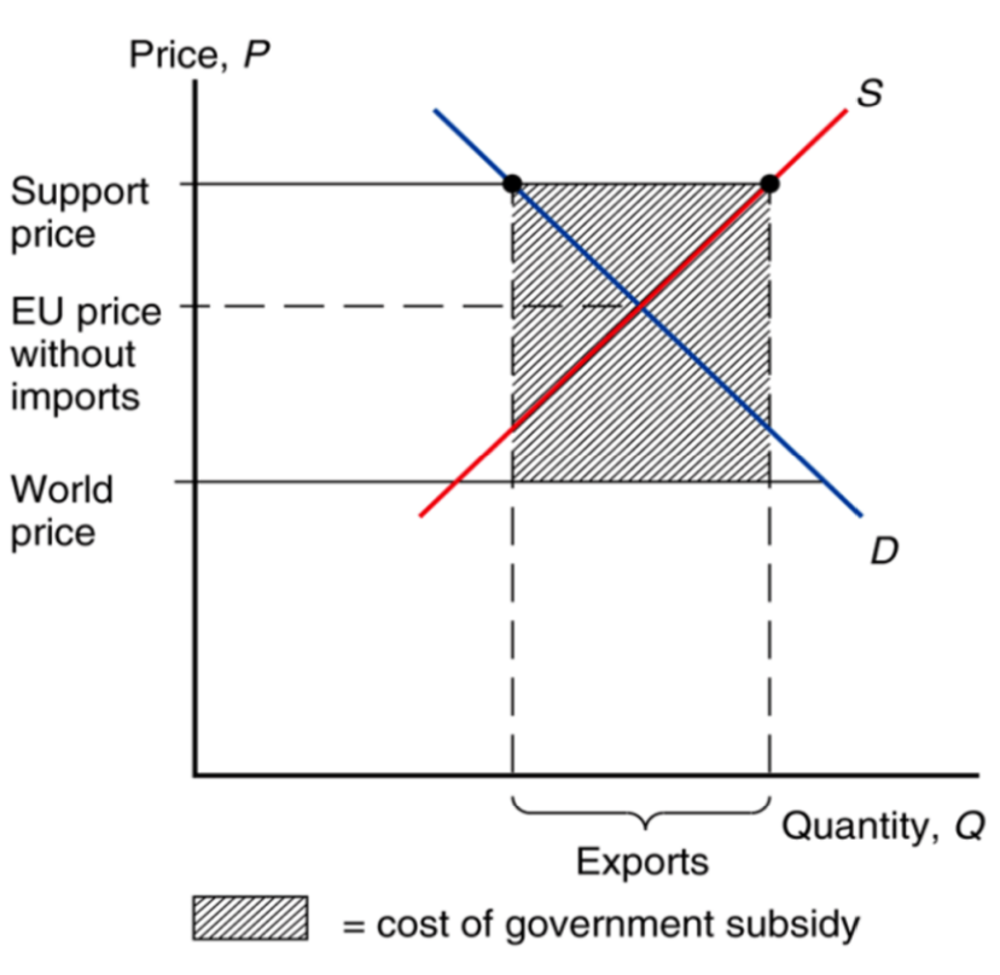
\includegraphics{cap}
  \end{figure}
\end{frame}
%--------------------------------------

%--------------------------------------
\begin{frame}
  A voluntary export restraint is similar to an import quota only imposed by the exporting country. 
  \begin{itemize}
    \item The restraint is often requested by the importing country
  \end{itemize}
  \medskip
  The profits/rents go to the foreign government/producer while the exporting country agrees to sell a restricted quantity at a higher price
  \begin{itemize}
    \item In the 1980s the US used this to restrict Japanese car imports
  \end{itemize}
\end{frame}
%--------------------------------------

%--------------------------------------
\begin{frame}
  For each implemented trade policy the domestic price will increase
  \begin{itemize}
    \item Domestic producers gain as they produce more
    \item Domestic consumers will demand less and lose
  \end{itemize}
  \medskip
  $p_{world}$ will decrease if $Home$ is large in economic terms.\\
  The implemented policies have divergent effect on government revenues
  \begin{itemize}
    \item Tariffs generate revenue, subsidies drain it, an quotas have no effect    
  \end{itemize}
  \medskip
  Importantly, trade policies create production and consumption distortions.
\end{frame}
%--------------------------------------

%--------------------------------------
\begin{frame}
  \begin{table}
    \scalebox{.6}{
    \begin{tabular}{lcccc}
      ~ & Tariffs & Export subsidy  & Import quote  & Voluntary export restraint\\
      \hline \\[-1.8ex]\\	
      Consumer surplus  & Decreases & Decreases & Decreases & Decreases\\
      Producer surplus  & Increases & Increases & Increases & Increases\\
      Government revenue& Increases & Decreases & Unchanged & Unchanged\\[-1.8ex]\\	
      Overnall national welfare & Ambiguous & Decreases & Ambiguous & Decreases\\
    \end{tabular}}
  \end{table}
\end{frame}
%--------------------------------------

%--------------------------------------
\begin{frame}
 In general trade policies are not efficient. 
 Consider support for farmers which exists in most countries, there are a number of ways to help them out
 \begin{enumerate}
   \item Tariffs
   \item Export subsidies
   \item Direct income transfers
 \end{enumerate}
 \medskip
 Implemented trade policies seem to always be biased against trade.
 \begin{itemize}
   \item e.g. tariffs are preferred over export quotas
 \end{itemize}
 \medskip
 This is mainly historically driven due to revenue raising. 
\end{frame}
%--------------------------------------

%--------------------------------------
\begin{frame}
  The level of protection received by an industry is often higher when
  \begin{itemize}
    \item It is a low wage low skill labour intensive industry
    \item It has high import penetration
    \item Produces consumption goods
    \item Production that is regionally concentrated, while consumers are dispersed
  \end{itemize}
\end{frame}
%--------------------------------------


%------------------------------------------------------------------------------
\end{document}
